% !TEX encoding = UTF-8 Unicode
\documentclass[12pt, a4paper]{article}

\usepackage{xcolor}
\definecolor{asparagus}{rgb}{0.53, 0.66, 0.42}

\newenvironment{MyColorPar}[1]{% for RED marked of revision
    \leavevmode\color{#1}\ignorespaces%
}{%
}%

\usepackage{titlecaps}
\Addlcwords{are or etc is of the}

%\usepackage{url}

\usepackage{array}
\usepackage{ragged2e}
\usepackage{rotating}
\usepackage{tabularx} % wide table
\usepackage{makecell}
% \usepackage{array}
\usepackage{colortbl} % \arrayrulecolor
\usepackage{multirow} % \multirow
\usepackage{hhline}
\usepackage{siunitx} % for  1e-10 scientific notation
%\usepackage{caption}
%\usepackage{subcaption}
\usepackage{booktabs, multirow} % for borders and merged ranges
\usepackage{soul}% for underlines
%\usepackage[table]{xcolor} % for cell colors
\usepackage{changepage,threeparttable} 
%%%



\usepackage[bf]{caption}
\newcommand{\bcaption}[2]{\caption{\textbf{#1} #2}}

\usepackage{outlines}

\usepackage{pgfgantt} % for Gantt chart/flow chart
\definecolor{barblue}{RGB}{153,204,254}
\definecolor{groupblue}{RGB}{51,102,254}
\definecolor{linkred}{RGB}{165,0,33}

\usepackage{newfloat} % for caption of smartdiagram
\DeclareFloatingEnvironment[fileext=diag,placement={!ht},name=Figure ]{diag} % diag

\usepackage{smartdiagram} %flowchart
\usesmartdiagramlibrary{additions} 
\usepackage{tikz}   % for DAG plot by  tikzpicture
\usetikzlibrary{arrows}
% This is not an official TikZ library. Use at your own risk!
% https://tex.stackexchange.com/questions/5461/is-it-possible-to-change-the-size-of-an-arrowhead-in-tikz-pgf

\makeatletter
% alternative latex arrow
\pgfarrowsdeclare{latexnew}{latexnew}
{
  \ifdim\pgfgetarrowoptions{latexnew}=-1pt%
    \pgfutil@tempdima=0.28pt%
    \pgfutil@tempdimb=\pgflinewidth%
    \ifdim\pgfinnerlinewidth>0pt%
      \pgfmathsetlength\pgfutil@tempdimb{.6\pgflinewidth-.4*\pgfinnerlinewidth}%
    \fi%
    \advance\pgfutil@tempdima by.3\pgfutil@tempdimb%
  \else%
    \pgfutil@tempdima=\pgfgetarrowoptions{latexnew}%
    \divide\pgfutil@tempdima by 10%
  \fi%
  \pgfarrowsleftextend{+-1\pgfutil@tempdima}%
  \pgfarrowsrightextend{+9\pgfutil@tempdima}%
}
{
  \ifdim\pgfgetarrowoptions{latexnew}=-1pt%
    \pgfutil@tempdima=0.28pt%
    \pgfutil@tempdimb=\pgflinewidth%
    \ifdim\pgfinnerlinewidth>0pt%
      \pgfmathsetlength\pgfutil@tempdimb{.6\pgflinewidth-.4*\pgfinnerlinewidth}%
    \fi%
    \advance\pgfutil@tempdima by.3\pgfutil@tempdimb%
  \else%
    \pgfutil@tempdima=\pgfgetarrowoptions{latexnew}%
    \divide\pgfutil@tempdima by 10%
    \pgfsetlinewidth{0bp}%
  \fi%
  \pgfpathmoveto{\pgfqpoint{9\pgfutil@tempdima}{0pt}}
  \pgfpathcurveto
  {\pgfqpoint{6.3333\pgfutil@tempdima}{.5\pgfutil@tempdima}}
  {\pgfqpoint{2\pgfutil@tempdima}{2\pgfutil@tempdima}}
  {\pgfqpoint{-1\pgfutil@tempdima}{3.75\pgfutil@tempdima}}
  \pgfpathlineto{\pgfqpoint{-1\pgfutil@tempdima}{-3.75\pgfutil@tempdima}}
  \pgfpathcurveto
  {\pgfqpoint{2\pgfutil@tempdima}{-2\pgfutil@tempdima}}
  {\pgfqpoint{6.3333\pgfutil@tempdima}{-.5\pgfutil@tempdima}}
  {\pgfqpoint{9\pgfutil@tempdima}{0pt}}
  \pgfusepathqfill
}

% alternative latex reversed arrow
\pgfarrowsdeclarereversed{latexnew reversed}{latexnew reversed}{latexnew}{latexnew}

% alternative latex' arrow
\pgfarrowsdeclare{latex'new}{latex'new}
{
  \ifdim\pgfgetarrowoptions{latex'new}=-1pt%
    \pgfutil@tempdima=0.28pt%
    \advance\pgfutil@tempdima by.3\pgflinewidth%
  \else%
    \pgfutil@tempdima=\pgfgetarrowoptions{latex'new}%
    \divide\pgfutil@tempdima by 10%
  \fi%
  \pgfarrowsleftextend{+-4\pgfutil@tempdima}
  \pgfarrowsrightextend{+6\pgfutil@tempdima}
}
{
  \ifdim\pgfgetarrowoptions{latex'new}=-1pt%
    \pgfutil@tempdima=0.28pt%
    \advance\pgfutil@tempdima by.3\pgflinewidth%
  \else%
    \pgfutil@tempdima=\pgfgetarrowoptions{latex'new}%
    \divide\pgfutil@tempdima by 10%
    \pgfsetlinewidth{0bp}%
  \fi%
  \pgfpathmoveto{\pgfqpoint{6\pgfutil@tempdima}{0\pgfutil@tempdima}}
  \pgfpathcurveto
  {\pgfqpoint{3.5\pgfutil@tempdima}{.5\pgfutil@tempdima}}
  {\pgfqpoint{-1\pgfutil@tempdima}{1.5\pgfutil@tempdima}}
  {\pgfqpoint{-4\pgfutil@tempdima}{3.75\pgfutil@tempdima}}
  \pgfpathcurveto
  {\pgfqpoint{-1.5\pgfutil@tempdima}{1\pgfutil@tempdima}}
  {\pgfqpoint{-1.5\pgfutil@tempdima}{-1\pgfutil@tempdima}}
  {\pgfqpoint{-4\pgfutil@tempdima}{-3.75\pgfutil@tempdima}}
  \pgfpathcurveto
  {\pgfqpoint{-1\pgfutil@tempdima}{-1.5\pgfutil@tempdima}}
  {\pgfqpoint{3.5\pgfutil@tempdima}{-.5\pgfutil@tempdima}}
  {\pgfqpoint{6\pgfutil@tempdima}{0\pgfutil@tempdima}}
  \pgfusepathqfill
}

% alternative latex' reversed arrow
\pgfarrowsdeclarereversed{latex'new reversed}{latex'new reversed}{latex'new}{latex'new}

% alternative o arrow
\pgfarrowsdeclare{onew}{onew}
{
  \pgfarrowsleftextend{+-.5\pgflinewidth}
  \ifdim\pgfgetarrowoptions{onew}=-1pt%
    \pgfutil@tempdima=0.4pt%
    \advance\pgfutil@tempdima by.2\pgflinewidth%
    \pgfutil@tempdimb=9\pgfutil@tempdima\advance\pgfutil@tempdimb by.5\pgflinewidth%
    \pgfarrowsrightextend{+\pgfutil@tempdimb}%
  \else%
    \pgfutil@tempdima=\pgfgetarrowoptions{onew}%
    \advance\pgfutil@tempdima by -0.5\pgflinewidth%
    \pgfarrowsrightextend{+\pgfutil@tempdima}%
  \fi%
}
{ 
  \ifdim\pgfgetarrowoptions{onew}=-1pt%
    \pgfutil@tempdima=0.4pt%
    \advance\pgfutil@tempdima by.2\pgflinewidth%
    \pgfutil@tempdimb=0pt%
  \else%
    \pgfutil@tempdima=\pgfgetarrowoptions{onew}%
    \divide\pgfutil@tempdima by 9%
    \pgfutil@tempdimb=0.5\pgflinewidth%
  \fi%
  \pgfsetdash{}{+0pt}
  \pgfpathcircle{\pgfpointadd{\pgfqpoint{4.5\pgfutil@tempdima}{0bp}}%
                             {\pgfqpoint{-\pgfutil@tempdimb}{0bp}}}%
                {4.5\pgfutil@tempdima-\pgfutil@tempdimb}%
  \pgfusepathqstroke
}

% alternative square arrow
\pgfarrowsdeclare{squarenew}{squarenew}
{
 \ifdim\pgfgetarrowoptions{squarenew}=-1pt%
   \pgfutil@tempdima=0.4pt
   \advance\pgfutil@tempdima by.275\pgflinewidth%
   \pgfarrowsleftextend{+-\pgfutil@tempdima}
   \advance\pgfutil@tempdima by.5\pgflinewidth
   \pgfarrowsrightextend{+\pgfutil@tempdima}
 \else%
   \pgfutil@tempdima=\pgfgetarrowoptions{squarenew}%
   \divide\pgfutil@tempdima by 8%
   \pgfarrowsleftextend{+-7\pgfutil@tempdima}%
   \pgfarrowsrightextend{+1\pgfutil@tempdima}%
 \fi%
}
{
 \ifdim\pgfgetarrowoptions{squarenew}=-1pt%
   \pgfutil@tempdima=0.4pt%
   \advance\pgfutil@tempdima by.275\pgflinewidth%
   \pgfutil@tempdimb=0pt%
 \else%
   \pgfutil@tempdima=\pgfgetarrowoptions{squarenew}%   
   \divide\pgfutil@tempdima by 8%
   \pgfutil@tempdimb=0.5\pgflinewidth%
 \fi%
 \pgfsetdash{}{+0pt}
 \pgfsetroundjoin
 \pgfpathmoveto{\pgfpointadd{\pgfqpoint{1\pgfutil@tempdima}{4\pgfutil@tempdima}}
                            {\pgfqpoint{-\pgfutil@tempdimb}{-\pgfutil@tempdimb}}}
 \pgfpathlineto{\pgfpointadd{\pgfqpoint{-7\pgfutil@tempdima}{4\pgfutil@tempdima}}
                            {\pgfqpoint{\pgfutil@tempdimb}{-\pgfutil@tempdimb}}}
 \pgfpathlineto{\pgfpointadd{\pgfqpoint{-7\pgfutil@tempdima}{-4\pgfutil@tempdima}}
                            {\pgfqpoint{\pgfutil@tempdimb}{\pgfutil@tempdimb}}}
 \pgfpathlineto{\pgfpointadd{\pgfqpoint{1\pgfutil@tempdima}{-4\pgfutil@tempdima}}
                            {\pgfqpoint{-\pgfutil@tempdimb}{\pgfutil@tempdimb}}}
 \pgfpathclose
 \pgfusepathqfillstroke
}

% alternative stealth arrow
\pgfarrowsdeclare{stealthnew}{stealthnew}
{
  \ifdim\pgfgetarrowoptions{stealthnew}=-1pt%
    \pgfutil@tempdima=0.28pt%
    \pgfutil@tempdimb=\pgflinewidth%
    \ifdim\pgfinnerlinewidth>0pt%
      \pgfmathsetlength\pgfutil@tempdimb{.6\pgflinewidth-.4*\pgfinnerlinewidth}%
    \fi%
    \advance\pgfutil@tempdima by.3\pgfutil@tempdimb%
  \else%
    \pgfutil@tempdima=\pgfgetarrowoptions{stealthnew}%
    \divide\pgfutil@tempdima by 8%
  \fi%
  \pgfarrowsleftextend{+-3\pgfutil@tempdima}
  \pgfarrowsrightextend{+5\pgfutil@tempdima}
}
{
  \ifdim\pgfgetarrowoptions{stealthnew}=-1pt%
    \pgfutil@tempdima=0.28pt%
    \pgfutil@tempdimb=\pgflinewidth%
    \ifdim\pgfinnerlinewidth>0pt%
      \pgfmathsetlength\pgfutil@tempdimb{.6\pgflinewidth-.4*\pgfinnerlinewidth}%
    \fi%
    \advance\pgfutil@tempdima by.3\pgfutil@tempdimb%
  \else%
    \pgfutil@tempdima=\pgfgetarrowoptions{stealthnew}%
    \divide\pgfutil@tempdima by 8%
    \pgfsetlinewidth{0bp}%
  \fi%
  \pgfpathmoveto{\pgfqpoint{5\pgfutil@tempdima}{0pt}}
  \pgfpathlineto{\pgfqpoint{-3\pgfutil@tempdima}{4\pgfutil@tempdima}}
  \pgfpathlineto{\pgfpointorigin}
  \pgfpathlineto{\pgfqpoint{-3\pgfutil@tempdima}{-4\pgfutil@tempdima}}
  \pgfusepathqfill
}

% alternative stealth reversed arrow
\pgfarrowsdeclarereversed{stealthnew reversed}{stealthnew reversed}{stealthnew}{stealthnew}

% alternative to arrow
\pgfarrowsdeclare{tonew}{tonew}
{
  \ifdim\pgfgetarrowoptions{tonew}=-1pt%
    \pgfutil@tempdima=0.84pt%
    \advance\pgfutil@tempdima by1.3\pgflinewidth%
    \pgfutil@tempdimb=0.21pt%
    \advance\pgfutil@tempdimb by.625\pgflinewidth%
  \else%
    \pgfutil@tempdima=\pgfgetarrowoptions{tonew}%
    \pgfarrowsleftextend{+-0.8\pgfutil@tempdima}%
    \pgfarrowsrightextend{+0.2\pgfutil@tempdima}%
  \fi%
}
{
  \ifdim\pgfgetarrowoptions{tonew}=-1pt%
    \pgfutil@tempdima=0.28pt%
    \advance\pgfutil@tempdima by.3\pgflinewidth%
    \pgfutil@tempdimb=0pt,%
  \else%
    \pgfutil@tempdima=\pgfgetarrowoptions{tonew}%
    \multiply\pgfutil@tempdima by 100%
    \divide\pgfutil@tempdima by 375%
    \pgfutil@tempdimb=0.4\pgflinewidth%
  \fi%
  \pgfsetdash{}{+0pt}
  \pgfsetroundcap
  \pgfsetroundjoin
  \pgfpathmoveto{\pgfpointorigin}
  \pgflineto{\pgfpointadd{\pgfpoint{0.75\pgfutil@tempdima}{0bp}}
                         {\pgfqpoint{-2\pgfutil@tempdimb}{0bp}}}
  \pgfusepathqstroke
  \pgfsetlinewidth{0.8\pgflinewidth}
  \pgfpathmoveto{\pgfpointadd{\pgfqpoint{-3\pgfutil@tempdima}{4\pgfutil@tempdima}}
                             {\pgfqpoint{\pgfutil@tempdimb}{0bp}}}
  \pgfpathcurveto
  {\pgfpointadd{\pgfqpoint{-2.75\pgfutil@tempdima}{2.5\pgfutil@tempdima}}
               {\pgfqpoint{0.5\pgfutil@tempdimb}{0bp}}}
  {\pgfpointadd{\pgfqpoint{0pt}{0.25\pgfutil@tempdima}}
               {\pgfqpoint{-0.5\pgfutil@tempdimb}{0bp}}}
  {\pgfpointadd{\pgfqpoint{0.75\pgfutil@tempdima}{0pt}}
               {\pgfqpoint{-\pgfutil@tempdimb}{0bp}}}
  \pgfpathcurveto
  {\pgfpointadd{\pgfqpoint{0pt}{-0.25\pgfutil@tempdima}}
               {\pgfqpoint{-0.5\pgfutil@tempdimb}{0bp}}}
  {\pgfpointadd{\pgfqpoint{-2.75\pgfutil@tempdima}{-2.5\pgfutil@tempdima}}
               {\pgfqpoint{0.5\pgfutil@tempdimb}{0bp}}}
  {\pgfpointadd{\pgfqpoint{-3\pgfutil@tempdima}{-4\pgfutil@tempdima}}
               {\pgfqpoint{\pgfutil@tempdimb}{0bp}}}
  \pgfusepathqstroke
}

% alias alternative to arrow
\pgfarrowsdeclarealias{<new}{>new}{tonew}{tonew}

\makeatother

% tip length code
\pgfsetarrowoptions{latexnew}{-1pt}
\pgfsetarrowoptions{latex'new}{-1pt}
\pgfsetarrowoptions{onew}{-1pt}
\pgfsetarrowoptions{squarenew}{-1pt}
\pgfsetarrowoptions{stealthnew}{-1pt}
\pgfsetarrowoptions{tonew}{-1pt}
\pgfkeys{/tikz/.cd, arrowhead/.default=-1pt, arrowhead/.code={
  \pgfsetarrowoptions{latexnew}{#1},
  \pgfsetarrowoptions{latex'new}{#1},
  \pgfsetarrowoptions{onew}{#1},
  \pgfsetarrowoptions{squarenew}{#1},
  \pgfsetarrowoptions{stealthnew}{#1},
  \pgfsetarrowoptions{tonew}{#1},
}}

\usepackage{times}
\usepackage{geometry}                % See geometry.pdf to learn the layout options. There are lots.
\usepackage{graphicx}
\usepackage{amssymb}
\usepackage{amsmath}
\usepackage{epstopdf}
\usepackage{wrapfig}
\usepackage{natbib}
\bibpunct{(}{)}{;}{a}{}{,} % to follow the A&A style
\usepackage[pdftex, plainpages=false, colorlinks=true, linkcolor=blue, citecolor=blue, bookmarks=false]{hyperref}
\usepackage{setspace}
\usepackage{multicol}
\usepackage{sectsty}
\usepackage{url}
\usepackage{lipsum}
\usepackage[tiny,compact]{titlesec}
\usepackage{fancyhdr}
\usepackage[font=footnotesize,labelfont=bf]{caption}
\usepackage{verbatim}
\usepackage[super]{nth}
\usepackage{lastpage}

% ---- Chinese characters --------------------------------------------------------
\usepackage{CJKutf8}
\newcommand{\cntext}[1]{\begin{CJK*}{UTF8}{bkai}#1\end{CJK*}}
%----------------------------------------------------------------------------------------
% --- Page Style ----

%\renewcommand{\headrulewidth}{0pt}
\renewcommand{\footrulewidth}{0pt}
\setlength{\paperheight}{29.7cm}
\setlength{\paperwidth}{21cm}
\addtolength{\voffset}{-1in}
\addtolength{\hoffset}{-1in}
\setlength{\topmargin}{1in}
\setlength{\oddsidemargin}{1.5cm}
\setlength{\evensidemargin}{1.5cm}
\setlength{\textwidth}{18cm}
\setlength{\textheight}{23.5cm}
\setlength{\footskip}{32pt}
\setlength{\marginparsep}{0.5cm}
\setlength{\marginparwidth}{1.5cm}
\setlength{\headheight}{0pt}
\setlength{\headsep}{1cm}
\setlength{\parindent}{0cm}
\setlength{\parskip}{.1cm}

%--- Fancy look --------------------------------------------------------------------------------------------
\pagestyle{fancy} % for header and footer
\fancyhf{} % clears the header and footer,
\lhead{\fancyplain{}{\doctitle}}
\rhead{\fancyplain{}{PI: Li-Hsing Chi}} % *** Fill your name here ***
\cfoot{\fancyplain{}{\cntext{共} \pageref*{LastPage} \cntext{頁}~~~~\cntext{第} \thepage \cntext{頁}}}
\lfoot{\underline{\cntext{表} C003}}

% --- define the title page 

\fancypagestyle{titlepage}{
\renewcommand{\headrulewidth}{0pt}
\rhead{}
\lhead{}
%\rfoot{}
%\lfoot{}
\cfoot{\fancyplain{}{\cntext{共} \pageref*{LastPage} \cntext{頁}~~~~\cntext{第} \thepage \cntext{頁}}}
\lfoot{\underline{\cntext{表} C002}}
}

%----------------------------------------------------------------------------------------------------------------
\bibliographystyle{apj} % it needs \citep{}

% --- additional stuff --------------------------------------------------------------------------------------
\newcommand{\todo}[1]{{\color{red}$\blacksquare$~\textsf{[TODO: #1]}}}
\newcommand{\doctitle}{Deep Learning in HNSCC} % *** Project Short Title ***


% --------------------------------------------------------------------------------
%%% for abbreviations, or acronyms
\usepackage[automake, acronym, nopostdot]{glossaries} 
\usepackage{glossary-inline}
%\setacronymstyle{long-short}
%\renewcommand*{\glossarysection}[2][]{} 
%\renewcommand*{\glossarysection}[2][]{\textbf{#1}: }
% for abbreviations environment
%\newcommand{\abbrlabel}[1]{\makebox[3cm][l]{\textbf{#1}\ \dotfill}}
\newenvironment{abbreviation}%{\begin{list}{}{\renewcommand{\makelabel}{\abbrlabel}}}{\end{list}}
% \newenvironment{<name>}[<number>][<default>]


\makeglossaries %https://tex.stackexchange.com/questions/110095/list-of-acronyms-is-not-displayed

\newacronym{cnn}{CNN}{Convolutional Neural Network}
\newacronym{gnn}{GNN}{Graph Neural Network}
\newacronym{gcnn}{GCNN}{Graph Convolutional Neural Network}
\newacronym{rnn}{RNN}{Recurrent Neural Network}
\newacronym{ehr}{EHR}{Electric Healthcare Records}

\newacronym{ihc}{IHC}{immunohistochemistry}
\newacronym{fdr}{FDR}{false discovery rate}

\newacronym{hpa}{HPA}{the Human Protein Atlas}

\newacronym{hnscc}{HNSCC}{head and neck squamous cell carcinoma}
\newacronym{tcga}{TCGA}{the Cancer Genome Atlas}
\newacronym{tcpa}{TCPA}{the Cancer Proteome Atlas}
\newacronym{tcia}{TCIA}{the Cancer Imaging Archive}

\newacronym{rna}{RNA}{ribonucleic acid}
\newacronym{rnaseq}{RNA-Seq}{RNA sequencing}
\newacronym{lncrna}{lncRNA}{long non-coding RNA}
%\newacronym{km}{KM}{Kaplan-Meier}
\newacronym{rppa}{RPPAs}{reverse-phase protein arrays}
\newacronym{rpma}{RPMA}{reverse-phase protein lysate microarray}



\newacronym{go}{GO}{Gene Ontology}
\newacronym{ipi}{IPI}{international protein index database}

\newacronym{mmp}{MMP}{matrix metalloproteinase}
 %DKK1, CAMK2N1, STC2, PGK1, SURF4, USP10, NDFIP1, FOXA2, STIP1, and DKC1
 %ZNF557, ZNF266, IL19, MYO1H, FCGBP, LOC148709, EVPLL, PNMA5, KIAA1683, and NPB

\newacronym{DKK1}{DKK1}{dickkopf WNT signaling pathway inhibitor 1} 
\newacronym{CAMK2N1}{CAMK2N1}{calcium/calmodulin dependent protein kinase II inhibitor 1} 
\newacronym{STC2}{STC2}{stanniocalcin 2} 
\newacronym{PGK1}{PGK1}{phosphoglycerate kinase 1} 
\newacronym{SURF4}{SURF4}{surfeit 4} 
\newacronym{USP10}{USP10}{ubiquitin specific peptidase 10} 
\newacronym{NEDD4}{NEDD4}{neural precursor cell expressed, developmentally down-regulated 4}
\newacronym{NDFIP1}{NDFIP1}{NEDD4 family interacting protein 1} 
\newacronym{FOXA2}{FOXA2}{forkhead box A2} 
\newacronym{STIP1}{STIP1}{stress-induced-phosphoprotein 1} 
\newacronym{DKC1}{DKC1}{dyskeratosis congenita 1, dyskerin} 

\newacronym{ZNF557}{ZNF557}{zinc finger protein 557} 
\newacronym{ZNF266}{ZNF266}{zinc finger protein 266} 
\newacronym{IL19}{IL19}{interleukin 19} 
\newacronym{MYO1H}{MYO1H}{myosin 1H} 
\newacronym{FCGBP}{FCGBP}{Fc fragment of IgG binding protein} 
\newacronym{LOC148709}{LOC148709}{LncRNA LOC148709} 
\newacronym{EVPLL}{EVPLL}{envoplakin-like protein} 
\newacronym{PNMA5}{PNMA5}{paraneoplastic antigen like 5} 
%\newacronym{KIAA1683}{KIAA1683}{IQCN, IQ Motif Containing N} 
\newacronym{IQCN}{IQCN}{IQ motif containing N} % previous name KIAA1683
% "IQ" refers to the first two amino acids of the motif: isoleucine (commonly) and glutamine (invariably)
\newacronym{NPB}{NPB}{neuropeptide B} 

 \newacronym{rt}{RT}{radiation therapy}
 \newacronym{nccn}{NCCN}{National Comprehensive Cancer Network}
 \newacronym{hif}{HIF}{hypoxia-inducible factor}
 \newacronym{egfr}{EGFR}{epidermal growth factor receptor}
 \newacronym{ras}{RAS}{rat sarcoma}
 \newacronym{hras}{HRAS}{Harvey rat sarcoma viral oncoprotein}
 \newacronym{erk}{ERK}{extracellular signal-regulated kinases}
 \newacronym{us}{US}{United States}
 \newacronym{fda}{FDA}{Food and Drug Administration}
 \newacronym{tpf}{Tax-PF}{docetaxel, cisplatin, and 5-fluorouracil}
 \newacronym{tki}{TKI}{tyrosine kinase inhibitor}
 \newacronym{her}{HER}{human epidermal growth factor receptor}
 \newacronym{ici}{ICI}{immune-checkpoint inhibitor}
 %\newacronym{ctla4}{CTLA-4}{cytotoxic T lymphocyte antigen 4}
 \newacronym{pd1}{PD-1}{programmed death 1}
 %\newacronym{pdl1}{PD-L1}{programmed death ligand 1}
 \newacronym{tim3}{TIM-3}{T-cell immunoglobulin mucin protein 3}
 \newacronym{lag3}{LAG-3}{lymphocyte activation gene 3}
 \newacronym{ifng}{IFN-$\gamma$}{interferon gamma}
 \newacronym{tigit}{TIGIT}{T cell immunoglobin and immunoreceptor tyrosine-based inhibitory motif}
 \newacronym{gitr}{GITR}{glucocorticoid-induced tumor necrosis factor receptor}
 \newacronym{vista}{VISTA}{V-domain Ig suppressor of T-cell activation}
 \newacronym{tmsb4x}{TMSB4X}{thymosin beta-4 X-linked}
 \newacronym{emt}{EMT}{epithelial-mesenchymal-transition}
 \newacronym{gdc}{GDC}{Genomic Data Commons}
 \newacronym{nci}{NCI}{the National Cancer Institute}
 \newacronym{gdac}{GDAC}{Genome Data Analysis Center}
 \newacronym{rest}{REST}{Representational State Transfer} 
 \newacronym{api}{API}{Application Programmable Interface}
\newacronym{grch38}{GRCh38}{Genome Reference Consortium Homo sapiens genome assembly 38}
\newacronym{fpkm}{FPKM}{Fragments per kilobase per million reads mapped}
\newacronym{rsem}{RSEM}{RNA-Seq by Expectation-Maximization}
\newacronym{slca}{SLC35E2A}{solute carrier family 35 member E2A}
\newacronym{slcb}{SLC35E2B}{solute carrier family 35 member E2B}
\newacronym{cde}{CDE}{Common Data Element}
\newacronym{id}{ID}{identification}
\newacronym{ajcc}{AJCC}{the American Joint Committee on Cancer}
\newacronym{uicc}{UICC}{he Union for International Cancer Control}
\newacronym{tnm}{TNM}{the tumor size (T), cervical lymph node metastases (N), and distal metastasis status (M)}
\newacronym{ci95}{95\% CI}{95\% confidence interval}
\newacronym{os}{OS}{overall survival}
\newacronym{rfs}{RFS}{recurrence-free survival}
\newacronym{hr}{HR}{hazard ratio}
\newacronym{hpv}{HPV}{human papillomavirus}
\newacronym{ene}{ENE}{extra-nodal extension}
\newacronym{lvsi}{LVSI}{lymph-vascular space invasion}
\newacronym{pni}{PNI}{perineural invasion}
\newacronym{doi}{DOI}{depth of invasion}
\newacronym{lnd}{LND}{lymph node density}
\newacronym{wpoi5}{WPOI-5}{worst pattern of invasion score 5}
\newacronym{glut4}{GLUT4}{glucose transporters 4}
\newacronym{slc2a4}{SLC2A4}{solute carrier family 2 member A4}
\newacronym{trim24}{TRIM24}{tripartite motif-containing 24}
\newacronym{til}{TIL}{tumor-infiltrating lymphocytes}
\newacronym{tmb}{TMB}{tumor mutational burden}

%\newacronym{hpa}{HPA}{the Human Protein Atlas}
\newacronym{cart}{CAR-T}{chimeric antigen receptor T cells}

\newacronym{ptta}{PTTA}{\textit{P} value of t-test or ANOVA}
\newacronym{anova}{ANOVA}{analysis of variance}
\newacronym{lcms}{LC-MS/MS}{liquid chromatography with tandem mass spectrometry}
\newacronym{maldi}{MALDI MS}{matrix-assisted laser desorption/ionization mass spectrometry}
\newacronym{maldii}{MALDI IMS}{matrix-assisted laser desorption/ionization imaging mass spectrometry}

\newacronym{pcr}{PCR}{polymerase chain reaction}
\newacronym{rtpcr}{RT-PCR}{reverse-transcription PCR}
\newacronym{qpcr}{RT-qPCR}{quantitative real-time reverse-transcription PCR}

\newacronym{tmuh}{TMUH}{Taipei Medical University Hospital}

\newacronym{dag}{DAG}{direct acyclic graph}

%ohm$V3V1V2 disserttion
\newacronym{cd}{CD}{cluster of differentiation}
\newacronym{ctla4}{CTLA-4}{cytotoxic T-lymphocyte associated protein 4 (CD152)}
\newacronym{clsm}{CLSM}{confocal laser scanning microscopy}
\newacronym{dapi}{DAPI}{4’,6-diamidino‐2-phenylindole}
\newacronym{dc}{DC}{dendritic cell}
\newacronym{eb}{EB}{Epstein Barr virus}
\newacronym{ent}{ENT}{ear- nose- and throat,  otorhinolaryngology}
\newacronym{fas}{Fas}{Fas cell surface death receptor (CD95)} % ligand; Fas -> tumor necrosis factor (TNF) family; 
\newacronym{fasl}{FasL}{Fas ligand (CD95L or CD178)} % FasL = CD95L or CD178; 
\newacronym{gphase}{G-phase}{gap phases in mitosis}
\newacronym{gvhd}{GVHD}{graft versus host disease}
\newacronym{hiv}{HIV}{human immunodeficiency virus}
\newacronym{hla}{HLA}{human leukocyte antigen}
%\newacronym{hpv}{HPV}{human papilloma virus}
\newacronym{icd}{ICD}{international classification of diseases}
\newacronym{il}{IL}{interleukin}
\newacronym{lc}{LC}{langerhans cell}
\newacronym{lp}{LP}{lichen planus}
\newacronym{lpl}{LPL}{leukoplakia}
\newacronym{lpldys}{LPL-dys}{leukoplakia with dysplasia but without malignant transformation}
\newacronym{lplca}{LPL‐ca}{leukoplakia with dysplasia with malignant transformation}
\newacronym{mab}{mAb}{monoclonal antibody}
\newacronym{mdsc}{MDSC}{myelo-derived suppressor cells}
\newacronym{mhc}{MHC}{major histocompatibility complex}
%\newacronym{mmp}{MMP}{matrix metalloproteinases}
\newacronym{nkg2d}{NKG2D}{natural killer group 2 member D}
%  MICA MICB is the ligand of NKG2D
\newacronym{mica}{MICA}{MHC-class-I-polypeptide-related sequence A}
\newacronym{micb}{MICB}{MHC-class-I-polypeptide-related sequence B}

\newacronym{nsaid}{NSAID}{non-steroidal anti-inflammatory drugs}
\newacronym{olp}{OLP}{oral lichen planus}
\newacronym{oscc}{OSCC}{oral squamous cell carcinoma}
\newacronym{pdl1}{PD‐L1}{programmed death-ligand 1 (CD274)}
\newacronym{pmod}{PMOD}{potentially malignant oral disorder}
\newacronym{ptld}{PTLD}{post‐transplant lymphoproliferative disorder}
\newacronym{pvl}{PVL}{proliferative verrucous leukoplakia}
\newacronym{sir}{SIR}{standard incidence ratio}
\newacronym{sot}{SOT}{solid organ transplantation}
\newacronym{taa}{TAA}{tumor associated antigen}
\newacronym{tam}{TAM}{tumor associated macrophage}
\newacronym{tcr}{TCR}{T cell receptor}
%\newacronym{til}{TIL}{tumor infiltrating lymphocyte}
\newacronym{tgf}{TGF}{transforming growth factor}
\newacronym{th}{Th}{T helper}
\newacronym{tls}{TLS}{tertiary lymphoid structure}
%\newacronym{tnm}{TNM}{tumor, node, metastasis classification system}
\newacronym{trail}{TRAIL}{tumor necrosis factor-related apoptosis‐inducing ligand}
\newacronym{treg}{Treg}{regulatory T cell}

\newacronym{aldh2}{ALDH2}{aldehyde dehydrogenase 2}

%%%%%%%%%%%%%%%%%%%%%%%%%%%%%%%%%%%%%%%%%%%%%%%%%%%%%%%%%%%%%%%%%%%%%%%%%%%%%%%%%%%%%%
%---------------------------------
%
%. Document
%
% -----------------------------------------------------------------------------------------------------------------
%\documentclass{article}
\usepackage[utf8]{inputenc}

% MOST template from https://github.com/kuochuanpan/most_proposal/blob/master/most_proposal.tex
\begin{document}
% MOST page
%
\includegraphics[trim=1.5cm 0 0 3cm]{cover.pdf}

\thispagestyle{titlepage}

\clearpage
% \cntext{TMU 口腔醫學院 2021 project}
% The real title page
%%%%%%%%%%%%%%%%%%%%%%%%%% title
\title{\Large \vspace{-2.5cm} \titlecap{Deep learning for whole-slide images and holistic} Electric Healthcare Records in Head and Neck Squamous Cell Carcinoma}
% or Deep learning for whole slide image and holistic EHR
%\author{Li-Hsing Chi}
%\date{May 2021}

\author{\small PI: Li-Hsing Chi (\cntext{祁力行})$^{1,2}$\\
{\footnotesize $^{1}$ \quad Division of Oral and Maxillofacial Surgery, Department of Dentistry\unskip, 
%    Taipei Municipal Wanfang Hospital\unskip, Taipei\unskip, Taiwan\\
Wan Fang Hospital\unskip, Taipei Medical University}\\
    
{\footnotesize $^{2}$ \quad Division of Oral and Maxillofacial Surgery, Department of Dentistry\unskip,
    Taipei Medical University Hospital\unskip, Taipei Medical University}\\
    
%$^{4}$ \quad Genomics Research Center\unskip, Academia Sinica\unskip, Taipei\unskip, Taiwan\\
    
%$^{5}$ \quad Graduate Institute of Biomedical Informatics, College of Medical Science and Technology\unskip, Taipei Medical University\unskip, No.172-1, Sec. 2, Keelung Rd.\unskip, Taipei 106\unskip, Taiwan\\

%Taipei\unskip, Taiwan\\
%{\footnotesize $^1$ Department of Physics and Astronomy, Michigan State University, East Lansing, MI 48824, USA}\\
%{\footnotesize $^2$Institute of Astronomy, Nation Tsing Hua University, Hsinchu 30013, Taiwan}\\ 
%{\footnotesize $^3$Department of Physics, Nation Tsing Hua University, Hsinchu 30013, Taiwan}
}
\date{\small \today}


\maketitle

\thispagestyle{titlepage}

% ------------------------------------------------------
%
% Abstract
%
% ------------------------------------------------------
\section{Abstract} % for navigation

\begin{abstract}


\textbf{Background:}
Head and neck squamous cell carcinoma (\acrshort{hnscc}) represents a significant health concern worldwide. Surgery and systemic therapy are still the standard of care for \acrshort{hnscc} patients. The break-through improvement of those interventions should depend on 1) the discovery of high impact prognostic biomarkers, and 2) proper treatment planning by accurate sub-population of those patients.
The survival analysis of the \acrfull{tcga} dataset is a well-known method to discover the gene expression-based biomarkers of \acrshort{hnscc}. It is necessary to determine a cutoff point of the patients' dichotomization in survival analysis with the continuous gene expression measurements. There is some optimization software for cutoff mining.
However, the software's determination of cutoffs is usually set at the median, 1/4 quantile, or 3/4 quantile of \acrfull{rnaseq} value to find a significant \textit{P} value by the Kaplan-Meier analysis. There are few clinicopathological or spiritual features available on their pre-processed data sets.
The survival analysis could conclude the manifest of clinical, pathological, and transcriptomics data to find the prognostic biomarkers.

%Methods: how the study was performed and statistical tests used
\textbf{Methods:}
R script was used to develop a comprehensive workflow, named "pvalueTex", running on the Rstudio platform. It includes data retrieving and pre-processing, feature selection, cutoff mining engine, Kaplan-Meier survival analysis, Cox proportional hazard modeling to discover prognostic biomarkers.
We further plan to develop a deep-learning based data mining as well as validation platform. It might incorporate whole-slide images of pathology from the Cancer Imaging Archive (TCIA) and Taipei Medical University (TMU) biobank.
%RNA-Seq data of \acrfull{tcga} for survival analysis. 
Graph convolutional neural network (GCNN) will be used for feature extraction from whole-slide images.
Recurrent neural network (RNN) will deal with "holistic features" from electric healthcare records (EHR) of Taipei Medical University Hospital (TMUH).
These patient's features should include physical, pathological, psychological data, and even more spiritual information investigated by physicians.
% construction of gene expression network.
%GNN graph neural network for CNN convolutional neural network
%The Cancer Imaging Archive (TCIA) whole-slide by Deep learning (ResNet)
% *** AI: deep learning, machine learning \citep{Huang2020}
%plot http://iltabiai.github.io/tips/latex/2015/09/15/latex-tikzdevice-r.html
%***Deep learning-based cancer survival prognosis from RNA-Seq data: approaches and evaluations
%*transfer learning from TCGA model
%torchvision, NanoMets Models
%save checkpoint, load then deepcopy()


% P-value => \textit{P} value
% Results: the main findings
\textbf{Preliminary Results:}
Using pvalueTex on the \acrshort{tcga} \acrshort{hnscc} cohort, we scanned human protein-coding genes (20,500) programmatically. After adjustment with other confounders, we found that the clinical tumor stage and the surgical margin involvement are independent risk factors in patient survival. 
According to the resulting tables with Bonferroni adjusted \textit{P} value under optimal cutoff as well as hazard ratio $(>=1.5)$, there were ten candidate biomarkers, named as DKK1, CAMK2N1, STC2, PGK1, SURF4, USP10, NDFIP1, FOXA2, STIP1, and DKC1, which are significantly associated with the poor prognosis of \acrfull{os}. At the same time, the other ten genes were over-expressed in the better survival patients (with hazard ratio $<=0.5$), named as ZNF557, ZNF266, IL19, MYO1H, FCGBP, LOC148709, EVPLL, PNMA5, IQCN (previous name as KIAA1683), and NPB.


%*** validated by \acrfull{hpa}.
Further validation will be conducted by using deep learning platform.
% are warranted 


%\thispagestyle{titlepage}
% Conclusions: brief summary and potential implications
\textbf{Conclusions:}
%Those 11 validated biomarkers (DKK1, CAMK2N1, STC2, PGK1, SURF4, NDFIP1, STIP1, DKC1, ZNF557, ZNF266, and FCGBP), 
The candidate biomarkers, clinical tumor size, and surgical margin status are suggested prognosis factors in \acrshort{hnscc} through TCGA analysis.
The transcriptomic representation of \acrfull{tcia} and TCGA could be applied to validate those candidates by independent TMU cohort (n=46, obtained at TMU Joint Biobank).
We conclude that expression data of \acrshort{rnaseq} with associated pathological images and holistic features will help to facilitate the biomarker discovery in terms of tumor-agnostic therapy.
% pvalueTex, equipped with an optimal cutoff finder, 

%Survival analysis using the Cancer Genome Atlas (TCGA) dataset is a well-known method to discover gene expression-based prognostic biomarkers of head and neck squamous cell carcinoma (HNSCC). It is necessary to determine a cutoff point by patients' dichotomization for the continuous gene expression. Usually, an optimization algorithm for cutoff determination has been set at the median or quantiles of RNA sequencing value.
%There are few clinicopathological features available on those pre-processed datasets. (feature selection or feature engineering issue)
% validated by the other HNSCC cohort:
%1) poor prognosis: CAMK2N1 (0.048214), PGK1 (0.009978), SURF4 (0.023127), USP10 (0.017768), NDFIP1 (0.022758), FOXA2 (0.001587);\\ % FOXA2 (0.038125)
%2) better prognosis: IL19 (0.049731), FCGBP (0.005658), KIAA1683 (IQCN, 0.005886), NPB (0.014177);\\

% row 20: The result showed ten overexpressed genes (symbol as DKK1, CAMK2N1, STC2, PGK1, SURF4, USP10, NDFIP1, FOXA2, STIP1, and DKC1) are significantly associated with a poor prognosis of overall survival. Furthermore, the other ten overexpressed genes (symbol as ZNF557, ZNF266, IL19, MYO1H, FCGBP, LOC148709, EVPLL, PNMA5, IQCN - former symbol as KIAA1683, and NPB) are correlated with better survival.


% Keywords
\textbf{Keyword:}
%\keyword{
Head and Neck Squamous Cell Carcinoma (HNSCC);
%Genome Database\sep
the Cancer Genome Atlas (TCGA);
the Cancer Imaging Archive (TCIA);
RNA-sequencing;
Survival Analysis;
Optimal Cutoff;
Biomarker Discovery; %\sep
%Tumor Type-agnostic Therapy\sep
%Immuno-Oncology\sep
%Targeted Therapy\sep
%Systemic Therapy\sep
Surgical Margin;
Deep Learning;
Graph Neural Network (GNN);
Graph Convolutional Neural Network (GCNN);
Recurrent Neural Network (RNN); 
Electric Healthcare Records (EHR);
Holistic Cancer Care;
Therapeutic Relationship;
Mindfulness Meditation
%}

\cntext{中文摘要。}

\end{abstract}

\clearpage




%\thispagestyle{titlepage}
% ------------------------------------------------------
%
% Introduction
% https://www.most.gov.tw/most/attachments/8eb87bfc-502c-4da8-b026-f9a499ae1622
% http://lgdntu.blogspot.com/2015/01/blog-post.html 專訪張典顯與楊慕華老師
% writing a fundable grant:
% critically significant, how do I approach this (解釋得很清楚,不可以草率,或僅止於做流水帳),  is there any 替代策略 (fallback approaches)
% just like 一篇 manuscript (手稿) 適合投到哪個 journal (期刊) 需要仔細審度
% being concise and precise (NIH: maximal 12 pages)
% ------------------------------------------------------
%「研究計畫之背景及目的: 詳述研究計畫之背景、目的、重要性及國內外有關本計畫之研究情況、重要參 考文獻之評述等」、
%「研究方法、進行步驟及執行進度」、
%「預期完成之工作項目 及成果」、
%「經費」
%「對社會的貢獻」
%\section{Introduction}」

\section*{\cntext{(一)研究計畫之背景及目的}} % 大約 3 頁 Background and Significance
%請詳述本研究計畫之背景、目的 具體目標 (Specific Aims)、重要性及國內外有關本計畫之研究情況、重要參考文獻之評述等。

% *** 講一個故事,先告訴大家領域的重要性和重大發現,然後再告訴大家什麼重要的問題尚待解決,而我所提的研究方案能提供什麼樣的解答,這就是 "rationale"
%\begin{outline}
%\1 Big picture.
%\1 Specific and important problems.
%\2 How much has been done and how much hasn’t?
%\2 How am I able to contribute solving the important and unsolved questions?
%\end{outline}
% * 研究背景的介紹需具備邏輯連貫性,且要與研究主軸相關聯。最佳的寫作方式是利用背景介紹點出尚未解決之問題,同時引出研究之重要議題。
% *長期目標願景 (long-term goal) 說清楚,包含哪些是領域當中重要但未解決的議題,以及個人的研究主題和此有何關聯
% then 將個人的研究主題和其它重要的主題連結 (to attract your reviewers)

% 文獻回顧及評述: review articles then discussion => 有助於說明計畫的重要性、創新性 
%*** 應就其中重要、關鍵的論文提出與之論辯、對話的過程,歸納出過去研究中值得參考的成果及論點,有哪些值得檢討、翻盤的盲點,以及迄今未獲解決或被忽略的面向,乃至前人研究的錯誤。



%\chapter{Introduction}
\label{chap:intro}
%\chaptermark{Epidemiology, Etiology, Pathogenesis, and Treatment of HNSCC}

%Introduction
%Background of the Problem
%Statement of the Problem
%Purpose of the Study
%Research Questions
%Significance of the Study
%Definition of Terms
%Assumptions, Limitations, and Delimitations
%Conclusion

%\section*{Background}

\section{Biological Hallmarks of Cancer}

The multi-step process of genetic alteration is contributing to the development of cancer. The accumulation of mutation, amplification, or chromosomal aberrations in proto-oncogenes or tumor-suppressor genes might be the consequence of the stimulation from intrinsic or extrinsic environments.
Since cancer cells acquired the ten biological hallmarks, these functional capabilities consist of sustaining proliferative signaling and evading growth suppressors, resisting cell death, enabling replicative immortality, inducing angiogenesis, activating invasion with metastasis, deregulating cellular energetics and metabolism, avoiding immune destruction, tumor-promoting inflammation, and genome instability and mutation \citep{Hanahan2000, Hanahan2011, Hanahan2017}. The tumor micro-environment, which is composed of cancer cells and tumor‐associated fibroblasts, infiltrating immune cells, and angiogenic vascular cells.

\begin{outline}
\1 \titlecap{metabolic reprogramming}
\end{outline}

The concept that cancer cells alter their utilization of energy sources—notably glucose—to support their proliferation was introduced almost 90 years ago by Otto Warburg, who observed that certain cultured-cancer cells have enhanced uptake of glucose, which is metabolized via glycolysis, even in the presence of oxygen levels that normally should favor oxidative phosphorylation.
%anaerobic glycolysis
The Warburg effect\citep{Warburg1956} is an example of carcinogenesis and metabolic reprogramming of cells by some environmental factors.
altered anaerobic glycolysis. 
In our previous work\citep{Chang2017b}, the Warburg effect promotes the progression of \acrshort{hnscc}, which is partially attributed to the \acrlong{slc2a4} (\acrshort{slc2a4}, or \acrlong{glut4}, \acrshort{glut4}) and \acrfull{trim24} pathway\citep{Chang2017b}\citep{Mani2020}.
% Cited In for PMID: 28061796
Lactic acidosis induced \acrshort{glut4} overexpression was also found in lung cancer cells\citep{Prado-Garcia2020}. 
%The overexpression of \acrshort{glut4} will lead to higher glucose uptake in proliferating cancer cells\citep{Mani2020}.
%There is a trend toward cancer type-agnostic study. 
Glutamine is the other blood-borne source of energy and biomaterials for growth and proliferation of most cancer cells\citep{Hanahan2017}.
%GLUT4 \citep{Chang2017b}
%lactate



%===================
%http://www.biomedicine.org.tw/Upload/07_DNA甲基化程度在大腸直腸癌扮演的角色.pdf
%脊椎動物之基因體中約20\%之序列為5'-GC-3' (簡稱CpG)之雙核苷酸(dinucleotide)。然而有 些長約1至2kb之序列段,其CpG含量高達60% (CpG islands)
%Epigenetic trinity in cancer: CpG islands
%60\% protein-coding genes with CpG islands on their promoter region
%(
%McGough JM, Yang D, Huang S, et al. DNA methylation represses IFN-gamma-induced and signal transducer and activator of transcription 1-mediated IFN regulatory factor 8 activation in colon carcinoma cells. Mol Cancer Res 2008;6:1841-1851.
%)
%methyl CpG-binding domain protein; MBD prevents TF binding on the promoter of gene
%=> causing impairment of mismatch repair: MMR => microsatellite instable: MSI

%環境因子的致癌機轉
%=>CpG hypermethylation to turn off tumor suppressor genes
%=>CpG Hypomethylation turn on oncogene by such as DKK1

%loss of gene imprinting <- hypomethylation
%alleles 

%histone methylation

%http://webcache.googleusercontent.com/search?q=cache:z8zvnjS-C3AJ:sites.mc.ntu.edu.tw/board.php?courseID%3D83%26f%3Ddoc%26folderID%3D581%26cid%3D3060&client=safari&hl=en&gl=tw&strip=1&vwsrc=0
%雖然以上我們討論的是癌症的基因體,但癌症的厲害就是它本來就利用人體原有的生物機制來生存(co-opting),因此,以上在癌症觀察到的基因體複雜性,其實也存在於正常人體.

%從最早,很單純的基因之exon序列,轉錄成mRNA,再轉譯成polypeptide,形成protein,到現在還要考慮epigenetics、mi RNA、TUF (ENCODE將之名為transcripts of unknown function (TUF)=> non-coding RNA 後來很紅)、chromosome environment,基因體的複雜性真是增加了不知多少倍,這也提醒我們在了解基因功能方面,必需更有全面性的關照。這也是「基因體醫學」必需以「基因體科學」為基礎的道理。





\section{Head and Neck Squamous Cell Carcinoma}
\label{sec:section}

Head and neck squamous cell carcinoma (HNSCC), which is derived from the oral cavity, oropharynx, hypopharynx and larynx, is the sixth common cancer worldwide \citep{Siegel2016}, as well as the fourth leading cancer causes of death for males in Taiwan\citep{MOHW_death2017}. The age-standardized incidence rate of \acrshort{hnscc} in males is 42.43 per 100,000 persons\citep{MOHW_incidence2018}. The mortality rate of HNSCC patients in the male is 11.1-fold greater than that in women.


%  Patients with early-stage cancer often manifest minimal physical evidence, which usually ignored by themselves, resulting in delayed diagnosis regarding poor tumor control and patient survival. Therefore, quitting bad habits, routine screening in high-risk population and early intervention will be helpful to improve their survival while maintaining the quality of life. 


\subsection{Etiology}
The main risk factors for HNSCC include carcinogens in tobacco and betel nut, alcohol, oncogenic viruses.
In Asian population, \acrfull{aldh2} mutation plays a very important rule to enhance HNSCC\citep{Chien2019} by alcohol consumption.
The oncogenic viruses such as \acrfull{hpv} and Epstein–Barr virus play a major carcinogenic role in tumors of the oropharynx and nasopharynx, respectively\citep{Ferrarotto2017}.
Moreover, physical irritations, ionized radiation and host susceptibility may also contribute to the etiology of HNSCC\citep{Ko1995,Znaori2003} (Figure \ref{fig:DAG_etiology}).
Primary prevention by minimizing exposure to known carcinogens is promising, but limited success is achieved due to addiction, economic, social or spiritual issues.


% This code uses the tikz package
%\begin{frame}[fragile]
%\frametitle{Directed acyclic graphs for %\acrshort{hnscc}}
\begin{figure}
\centering
\begin{tikzpicture}[scale=3.5, every node/.style={scale=1.3}] %, transform shape]
\node (v0) at (-1.49,1.64) {Age/Gender};
\node (v1) at (0.705,1.42) {Alcohol/Betel/Cigarette};
\node (v2) at (-1.18,-1.38) {Healthy Food/Exercise};
\node (v3) at (-0.167,0.515) {Other Risky Behavior};
\node (v4) at (1.19,-1.52) {\large \acrshort{hnscc}};

\draw [-latexnew, arrowhead=0.5cm, line width=4pt, ultra thick, dashed] (v0) .. controls (-0.408,1.72) and (0.325,1.64) .. (v1);
\draw [-latexnew, arrowhead=1cm, line width=4pt, ultra thick, green, dashed] (v0) edge (v2);
\draw [-latexnew, arrowhead=0.5cm, line width=4pt, ultra thick, dashed] (v0) .. controls (-0.761,1.13) and (-0.318,0.754) .. (v3);
\draw [-latexnew, arrowhead=0.5cm, line width=4pt, ultra thick, red] (v0) .. controls (-0.852,0.234) and (0.0430,-0.821) .. (v4);
\draw [-latexnew, arrowhead=2cm, line width=4pt, ultra thick, red] (v1) .. controls (1.30,0.923) and (1.46,-0.0573) .. (v4);
%  \draw [options/.expand once=\x] (0,-1.2*\i) -- (3,-1.2*\i) node [right] {\x};
\draw [-latexnew, arrowhead=1cm, line width=0.4cm, ultra thick, green] (v2) edge (v4);
\draw [-latexnew, arrowhead=1cm, line width=4pt, ultra thick, red] (v3) edge (v4);
\end{tikzpicture}

\bcaption{HNSCC will be caused by carcinogen or other factors.}
{
From the intrinsic factors (such as age and gender), the accumulated genetic alteration will be part of etiology of cancer. Carcinogen from alcohol, betel nut and/or cigarette will definitely induce \acrshort{hnscc} by time passes. People usually learn "risky" or "healthy" behaviors by many reasons, which modify their possibility to get cancer.\\
(\textcolor{red}{red line}: increasing the chance of getting HNSCC; \textcolor{green}{green line} will reduce it; black dot: indicate unknown reasons for taking those habits)
}
\label{fig:DAG_etiology}
\end{figure}



%\paragraph{Ancient History of \acrshort{hnscc}}
% \citep{Fornaciari2012}
% \citep{Rehemtulla2010}
%Inchingolo, F., Santacroce, L., Ballini, A., Topi, S., Dipalma, G., Haxhirexha, K., Bottalico, L., \& Charitos, I. A. (2020). Oral cancer: A historical review. In International Journal of Environmental Research and Public Health (Vol. 17, Issue 9). MDPI AG. https://doi.org/10.3390/ijerph17093168 \citep{Inchingolo2020}




%Overview of HNSCC (Indian)
%https://www.intechopen.com/books/oral-cancer/oral-cancer-an-overview

% ALDH2 mutaion 戒酒有理
% 在美國北加州參加演講。
% 很棒!心得是:該戒酒了,至少要去檢測 ALDH2 基因是否突變影響解酒酵素→ 因為乙醛堆積致癌!
% 菸與酒在全身癌症的貢獻度是可以相比的。只有壞處沒有好處
% http://taies.org/
% 喝酒臉紅(酒精不耐症)表示危險,因為代謝酒精的酵素不正常,身體容易大量累積乙醛,這是一級致癌物。
% 尤其是,如果酒精不耐者加上吸菸,口腔癌罹患機會,是一般人的400 倍。
% 酒駕更會製造社會問題。
% 
% #鼓勵檢測 ALDH2 基因
% #建議酒精不耐者戒酒
% #戒菸戒酒同樣重要
% #適量紅酒對亞洲民族的心血管完全沒有好處
% #亞洲人一天最多10克酒精相當於350mL鋁罐啤酒
% 
% 專題演講 : Alcohol Intolerance: An Under-Recognized Health Risk and Precision Oral Cancer
% 演 講 者: Che-Hong Chen, PhD.
% 陳哲宏
% Alcohol lntolerance Education Society
% 台灣酒精不耐淀衛教協會
% LINE ID: jchehong
% Email: chehong@stanford.edu
% STANFORD
% SCHOOL OF MEDICINE
% Stanforl Cuirersity Medical Center
% Chemical and Systems Biology
% 歡迎捐款!協會慈善捐款收據備索
% 郵政劃撥劃撥帳號:50434421
% http://taies.org/
% 戶名:社團法人台灣酒精不耐症衛教協會
% 謝謝陳老師的演講,我是提問的 北醫 祁力行。
% 戒菸戒酒都能使用藥物幫忙,加上專業衛教,建立動機、鞏固決心,我還知道一些中醫穴道,雷射針灸可以幫忙戒除之,多管齊下。
% Acetaldehyde
% 老師提到戒酒已有藥物,Disulfiram 正是抑制 ALDH1,讓乙醯醛堆積,酒後症狀嚴重。:-)


\subsection{Conventional Treatment}


%The modern treatment of HNSCC should be done by surgery alone, radiation therapy alone, or a combination of them with adjuvant chemotherapy according to National Comprehensive Cancer Network (NCCN) guidelines \citep{Pfishter2019}. Despite those interventions, the 5-year survival rate for this disease has improved only marginally over the past decade, and recurrent disease is observed in ~50\% of all patients \citep{Forastiere2001,Warnakulasuriya2009}. By comparison with new systemic treatments seen in other solid tumours, the prognostic result of targeted therapy, ex. EGFR inhibitors, in HNSCC patients has remained relatively stationary in recent years. \citep{Argiris2015a}. 
%%

% chemotherapy => systemic therapy
The treatment strategies of HNSCC are surgery alone, systemic therapy with concurrent radiation therapy (systemic therapy/RT), or surgery with adjuvant systemic therapy/RT (according to National Comprehensive Cancer Network, NCCN Clinical Practice Guidelines in HNSCC, Version 2.2020) \citep{Pfister2020a}. Despite the improvement in those interventions, the survival of HNSCC has improved only marginally over the past decade worldwide \citep{hpa2019}.
The recurrent disease is still observed in up to 50\% of all patients \citep{Forastiere2001,Warnakulasuriya2009}.
By comparison with new systemic treatments seen in other solid tumours, the prognostic result of targeted therapy, ex. EGFR inhibitors, in HNSCC patients has remained relatively stationary since it's available\citep{Argiris2015a}.
The critical advancement of immuno-oncology should benefit from emerging prognostic biomarkers, which guide the development of modern systemic therapy.
% Pfister, D. G.

%%Oral cavity and oropharyngeal cancer account for more than 7000 deaths annually, with an annual incidence of more than 30,000 new cases within the United States. 1  Worldwide it is the sixth most common malignancy, with incidence varying greatly among different geographic locations. Its prevalence can range from countries with rates similar to those in the United States, to countries such as India, where death from oral cavity cancer is one of the top three forms of cancer death. As well in Taiwan, HNSCC is one of the top four forms of cancer death. 
%Despite improvements in treatment, long-term survival rates are relatively unchanged over the past 30 years.


%Chemotherapy
%Checkpoint inhibitor immunotherapy

%HNSCC expresses higher levels of Nuclear factor-kappa B (NF-κB), which proposed a hypothesis that inhibition of NF-κB will attenuates cancer cell proliferation. \citep{Yamamoto2001} The presence of cyclin D1 overexpression has been correlated with increased cervical lymphatic metastases, in terms of poor prognosis. \citep{Akervall1997}...as an independent predictor of nodal metastasis, grade, and adverse pathological features.

%% http://web.tccf.org.tw/lifetype/index.php?op=ViewArticle&articleId=4480&blogId=1 振興醫院血液腫瘤科 陳國維醫師


%\subsection{??Prognostic Biomarkers guide the Treatment of \acrshort{hnscc}}
%A biomarker can be either predictive or prognostic. A predictive marker predicts benefit from a specific treatment; it helps to select a particular treatment over another. A prognostic marker predicts the natural history of disease (survival), independent of treatment. It can indicate a need for further treatment, but does not help to determine which treatment.The key advancement of those interventions should be i) the discovery of high impact diagnostic/prognostic biomarkers, ii) and planning of the proper treatment modalities for accurate sub-grouped HNSCC patients.
%The ROC Plotter is the first online transcriptome-level validation tool for predictive biomarkers.
% http://www.rocplot.org

%The management of head and neck malignancies is site and histology specific, and requires a multidisciplinary team approach. In this chapter, we review the current knowledge of \acrshort{hnscc}, and discuss ongoing and future research aiming to improve the management and outcomes of patients with these malignancies.


% from manuscript of TMSB4X 2017
% https://docs.google.com/document/d/1j0GBllab9qr7JqB14z2KBCVGO0OkVXWQpcxCdJ3llVE/edit?usp=sharing)






%}


%\subsubsection{Medical Oncology for \acrshort{hnscc}}



\subsection{Immunotherapy for \acrshort{hnscc}}
Modern Systemic Therapy is guided by biomarkers.
%Immune Response in \acrshort{hnscc}
%Cancer Immunotherapy
The basic principles that guide cancer Immunotherapy are immune surveillance, immune editing, and immune tolerance\citep{Sharma2017}, involving immune-checkpoint molecules.
%Figure15_cite_Ferrarotto2017.png
Until the immuno-oncology era, \acrfull{ici} was introduced since 2014 for treating \acrshort{hnscc}\citep{Seiwert2014}\citep{Swanson2015}.
The \acrshort{ici} works on immune checkpoint molecules, including \acrfull{pd1}, \acrfull{ctla4}, \acrfull{tim3}, \acrfull{lag3}, \acrfull{tigit}, \acrfull{gitr}, and \acrfull{vista}\citep{Mei2020}.
The \acrshort{us} \acrshort{fda} has approved the anti-\acrshort{pd1} agents (e.g. pembrolizumab and nivolumab) as a monotherapy for the platinum-treated patients with recurrent or metastatic \acrshort{hnscc}\citep{Cramer2019}. 
According to the phase 3 KEYNOTE-048 study, \acrshort{pdl1} is a validated biomarker used in clinical guidance for candidate selection of pembrolizumab\citep{Burtness2019}\citep{Gavrielatou2020}.
However, because of the complexity of immune-tumor interaction, \acrshort{ici} has 20\% response rate to \acrfull{pdl1} expressed patients (over 50\% in \acrlong{ihc}, \acrshort{ihc} staining of \acrshort{hnscc})\citep{Swanson2015}\citep{Gavrielatou2020}.

Currently, Pembrolizumab and nivolumab's success is also based on a common biomarker (e.g., \acrshort{pd1}) crossing several types of cancer.
It shows a model of tumor type-agnostic therapy\citep{Yan2018}.
%*** PD-L1/PD-L2 is a biomarker; Keynote-012
There are several common biomarkers of \acrfull{ici} under evaluation, including \acrfull{til}, \acrfull{ifng}, and \acrfull{tmb}\citep{Gavrielatou2020}.
The other \acrshort{ici}, anti-\acrshort{lag3} (pelatlimab), is currently evaluated under the phase I/IIA\citep{Cristina2019} (ClinicalTrials.gov Identifier: NCT01968109) and II-IVA\citep{Neal2019} (NCT04080804) studies.
%%%%%%%%%%%
%X

% The font size must be 10 point or larger and footnotes\footnote{This is a footnote.} must be two sizes smaller than the text\footnote{This is another footnote.} but no smaller than eight points. Chapter, section, or other headings should be of a consistent font and size throughout the ETD, as should labels for illustrations, charts, and figures.  

%\subsection{Creating a Subsection}
%\label{sec:subsection}

%\subsubsection{Creating a Subsubsection}

%\paragraph{This is a heading level below subsubsection}



%\makeatletter
%\let\@currsize\normalsize
%\makeatother

% tabular environments are set to be single-spaced in the  thesis class,  but long tables do not use tabular
% to get around this, set the spacing to single spacing at the start of the long table environment, and set it back to double-spacing at the end of it





\section{Holistic Cancer Care}

%****************%
%\subsubsection{Holistic Cancer Care} 
% carcinogenesis by epigenetic control (placebo/nocebo), Bruce Lipton introduced mind-brain-body system. (gene expression is not an independent $X_mrna$, which is correlated with other $X_body, X_stress, X_inflammation, X_ros$)
% cancer care with person-central approach, PCA; Cullen, Carl Rogers

%TCGA treated by surgery and more; TNM available yes

%discussion: the third limitation
There are eighty-one ($X_1 ... X_{81}$) physical, pathological and social conditions derived from participants available for survival modeling in the TCGA, % since it has comprehensive clinical features, 
such as age, gender, residual tumor, vital status, days\_to\_last\_followup, cancer stage, smoking duration, exposure to alcohol, asbestos, radioactive radon. 
However, the TCGA did not collect other features from holistic cancer care.
% Input $X_1...X_n$ (e.x. patients features: such as age, gender, gene expression, cancer stage; emotional 情緒(心)
Going for holistic cancer care\citep{Mehta2019}\citep{Iftikhar2021} spiritual and emotional condition is equally essential comparing with physical and social status (see Figure \ref{fig:figure5}).

%
World Health Organisation has called worldwide for delivering people-centred (or person-centred) care from the physical, emotional, socioeconomic, and spiritual perspectives\citep{WHO2015}\citep{Ling-ChengMong2021}.
Core principles can be taken to achieve people-centred and integrated health service delivery. 
The first principle is holistic – focusing on physical, socioeconomic, mental, and emotional well-being. 
Holistic care has been defined that care and sees the person as a whole with psychological, social, and environmental levels of needs and goals.
%that considers  factors rather than just the symptoms of disease or ill-health.

%The second principle is empowering – supporting people to manage and take responsibility for their health,
%Empowerment: the process of supporting people and communities to take control of their own health needs resulting, 
%for example, in the uptake of healthier behaviors or the ability to self-manage illnesses.
%People-centred care requires that people have the education and support they need to make decisions and participate in their care.

%Glossary:
%People-centred care: an approach to care that consciously adopts individuals’, carers’, families’ and communities’ perspectives as participants in, and beneficiaries of, trusted health systems that respond to their needs and preferences in humane and holistic ways. People-centred care also requires that people have the education and support they need to make decisions and participate in their own care. It is organized around the health needs and expectations of people rather than diseases (7,8) 
%Person-centred care: care approaches and practices that see the person as a whole with many levels of needs and goals, with these needs coming from their own personal social determinants of health.
%(1. World Health Organization. WHO global strategy on people-centred and integrated health services: interim report. https://apps.who.int/iris/handle/10665/155002 (2015).)


%*** make Figure 5 holistic: Figure_5_holisticCare.pdf
\begin{figure}[hp]
\centering
\includegraphics[width=14cm]{Figure_5_holisticCare.pdf}
\bcaption{The concept of holistic care for \acrshort{hnscc} patients.}
{\\Beyond carcinogenesis - Under the mind-brain-body axis, a stressful environment (giant \textcolor{black}{black} arrow) will trigger emotional reception. The subconscious mind (brain) will release stress hormones and inflammation signals in response to the emotion. The physical body's internal environment (cells) alters epigenetic control in gene regulation and mRNA expression. In a long incubation time, the tissue/cells will be transformed into dysplasia then malignancy (e.x. HNSCC) with helping from known carcinogens.\\
Cancer care - Holistic care should take care of cancer patients' spiritual, emotional, physical, and socioeconomic needs. Physical care will be carried out by medication therapy or surgery. After establishing a therapeutic relationship (TR), the physicians' spiritual properties (empathy, sympathy, and compassion) will engage their patients and recover their self-compassion to gain resilience against the disease through their mind-brain-body axis.
Thus, we suggest electric healthcare records (EHR) include physical, pathological, psychological data, and even more spiritual information. The \acrshort{tcga} should collect "holistic features" as well (\textcolor{green}{green} dashed line).}
\label{fig:figure5}
\end{figure}
%meridian and emotion has mutual reaction
%meridian effect tissue and organ
%(autonomic nerve system, myofascial network, prefrontal cortex)
%placebo-effect influence on drug discovery
%gene expression in deep learning
%Ching, T. et al. Opportunities and obstacles for deep learning in biology and medicine. J. R. Soc. Interface 15, (2018).
%慈悲心 利他心
%博士班學生,越研究越發現,科學的不足,心理與靈性的力量,更是背後推動的冥冥力量,身心靈是合一的
%#正念 除了可以減壓,還可以治癒疼痛
% modify the dark environment 改造患者的心,就能改造他的身體環境,有利消除癌症


%we educate them
%1. Mong, L.-C., Liao, F., Chiou, J. & Chiang, P. Tips for Integrating Spiritual Care Delivery in Dental Education. in Asia Pacific Medical Education Conference. Short Communication 5 (National University of Singapore, 2021).\citep{Ling-ChengMong2021}
Spiritual care is the key to holistic healthcare in dental practice\citep{Ling-ChengMong2021} and cancer patient care\citep{Hulett2016}. 
It is mindful of patient's mental health, emotional changes, socioeconomic during healthcare.  %Taking patient’s socioeconomic statement and supporting system thoroughly for building a holistic consideration. 
We are learning to listen proactively.
It is aware of the patient's spiritual needs.
%Applying the holistic healthcare strategies, such as the shared decision making, to collect more spiritual-related information of patients in the treating process and adjusting the approaches dynamically.\citep{Ling-ChengMong2021}
% mindfulness-based cognitive therapies [MBCT]
%%%% MBSR "念" 今天的心 專心才有幸福感(味覺嗅覺靈敏專心吃
Jon Kabat-Zinn has introduced the mindfulness-Based Stress Reduction (MBSR) program in 1979\citep{Niazi2011}. MBSR composes the contemplative, spiritually based Buddhist philosophy, which promotes a nonjudgmental, accepting, and patient worldview and teaches relaxation through focused awareness on breathing during meditation. It employs (static) mindfulness meditation to alleviate suffering associated with physical (pain), psychosomatic and psychiatric disorders.
%是1979年麻薩諸塞大學的榮譽教授Jon Kabat-Zinn => 佛教禪修的mindfulness 正念止觀(中譯建譯:自我覺察)帶入西方身心醫學及心理學領域。
The Chinese Qigong and Tai Chi, belonging to movement-meditative-breathing interventions, also encourage (dynamic) mindfulness and self-awareness. 
%Search Inside Yourself was born at Google in 2007 when one of Google’s earliest engineers, Chade-Meng Tan, gathered a team of leading experts in mindfulness, neuroscience, leadership and emotional intelligence to develop an internal course for fellow Google employees lovingly called Search Inside Yourself (SIY).
% 目的與功效  出入息 呼吸念頭 回到覺知,不再被潛意識自動導航干擾情緒
%正念,放下二元評價 正念覺知 XAI saliency mapping and trustworthiness in deep learning
%覺知 漸入空性 Y=wX + bias
%解決情緒苦(七情) 四聖諦
%慈悲心 安心(情緒穩定)
%了卻見人苦的「慈悲心」易感者同理心 empathy
%道歉不是一段文字,不是一個儀式(療癒冤親債主來自慈悲心)
%冤親債主 決定不再影響環境 基因 expression,減少意外與疾病、癌症
A systematic review of spiritually based interventions and psychoneuroimmunological (PNI) outcomes in breast cancer survivorship was reported by Hulett et al.\citep{Hulett2016}. 
%Objective This is a review of spiritually based interventions (eg, mindfulness-based stress reduction, MBSR) that utilized psychoneuroimmunological (PNI) outcome measures in breast cancer survivors. Specifically, this review sought to examine the evidence regarding relationships between spiritually based interventions, psychosocial-spiritual outcomes, and biomarker outcomes in breast cancer survivors. 
%Methods A systematic search of 9 online databases was conducted for articles of original research, peer-reviewed, randomized and nonrandomized control trials from 2005-2015. Data were extracted in order to answer selected questions regarding relationships between psychosocial-spiritual and physiological measures utilized in spiritually based interventions. Implications for future spiritually based interventions in breast cancer survivorship are discussed. Results Twenty-two articles were reviewed. 
%mindfulness-based cancer recovery (MBCR) 
Psychosocial stress is associated with cancer incidence and poor survival\citep{Chida2008}.
These impacts might be mediated through the hypothalamic-pituitary-adrenal (HPA) axis\citep{Hsiao2012}.
Thus, cortisol is one of the most common (objective) outcomes studied in PNI factors. % others: interleukin, cytokines, lymphocytes (CD4+, CD8+), CD56+, vitals signs, telomere length, telomere activity, HRV
The standardized, psychosocial (subjective) measures include depression, stress, quality of life, anxiety, fatigue, mindfulness, mood, and specific spiritual growth (i.e., the meaning of life)\citep{Hsiao2012}. %  body-mind-spirit (BMS) group therapy in the Meaning in Life questionnaire (MLQ) including two sub-scales: MLQ-Presence and MLQ-Search.
% The MLQ [15] for measuring psychological well-being consists of two subscales: the 5-item MLQ-Presence subscale, measuring the subjective sense that one’s life is meaningful, and the 5-item MLQ-Search subscale, measuring the drive and orientation toward finding meaning in one’s life.
%Compared with control groups, intervention groups demonstrated positive mental health outcomes and improved or stable neuroendocrine-immune profiles, although limitations exist. %Design methods have improved with regard to increased use of comparison groups compared with previous reviews. There are few spiritually based interventions that specifically measure religious or spiritual constructs. Similarly, there are few existing studies that utilize standardized religious or spiritual measures with PNI outcome measures. 
Findings suggest that mindfulness meditation could stabilize neuroendocrine-immune activity (measured by PNI biomarkers) in breast cancer patients comparing to control groups\citep{Hulett2016}.
%This review revealed a positive pattern between spiritually-based interventions and several PNI biomarker outcomes, suggesting that spiritually-based interventions offer positive mental and physiological health benefits. 
%For breast cancer survivors, these studies suggested that engaging in spiritually-based practices may improve or stabilize the immune profile dysregulation that occurs with breast cancer.\citep{Hulett2016}.
%From a PNI perspective, future spiritually based interventions should include standardized measures of religiousness and spirituality in order to understand relationships between and among religiousness, spirituality, and neuroendocrine-immune outcomes. Future research should now focus on determining the minimum dose and duration needed to improve or stabilize neuroendocrine-immune function, as well as 
%diverse setting needs, including tele-medicine practice for survivors who are too ill to travel to group sessions or lack economic resources.
% 自動導航(潛意識)易受情緒影響,造成焦慮、發炎、免疫 Cancer
%Mindfulness based stress reduction provides psychological benefit and restores immune function of women newly diagnosed with breast cancer: A randomized trial with active control.
%BACKGROUND: Women newly diagnosed with breast cancer experience psychological distress, accompanied by reduced Natural Killer Cell Activity (NKCA) and altered levels of cytokines, which may compromise cancer control. Few studies have evaluated psycho-immune outcomes of mindfulness-based stress reduction (MBSR) for women newly diagnosed with breast cancer in comparison to an active control condition. OBJECTIVE: The purpose of this study was to determine whether MBSR benefits psychological, behavioral, and immunological function in women recently diagnosed with breast cancer. DESIGN: After confirmation of breast cancer staging, women diagnosed with early-stage breast cancer (n = 192) were randomized to an 8-week MBSR program or an 8-week active control condition (ACC). The ACC consisted of a series of cancer recovery and health education classes. Both MBSR and the ACC were administered in group format. METHODS: Women completed psychometric instruments and provided blood for NKCA and cytokine levels at pre-, mid-, and completion of program, as well as at 1- and 6-months post-program. One hundred and twenty four women completed all five-assessments (MBSR, n = 63; ACC, n = 61). Hierarchical linear modeling was used to analyze trajectories of outcomes over time and between groups. 
%RESULTS: Compared to the ACC group, women randomized to MBSR exhibited decreasing trajectories of perceived stress, fatigue, sleep disturbance, and depressive symptoms. 
%Further, compared to women randomized to ACC, MBSR women exhibited trajectories demonstrating significantly more rapid restoration of NKCA, accompanied by 
%lower circulating TNF-alpha levels, lower IL-6 production =>  pro-inflammatory cytokines
%and greater IFN-gamma production => IFN gamma supports an immune-mediated response against cancer and this may be important during the transition following cancer treatment
A randomized clinical trial with active control proved that early provision of MBSR for women newly diagnosed with breast cancer provides psychological benefits (reduction of stress, fatigue, sleep disturbance, and depressive symptoms), and also optimizes immune functions (higher natural killer cell activity, higher \acrshort{ifng}, lower TNF-alpha, lower IL-6) supportive of cancer survival\citep{WitekJanusek2019}.



%%%% PCA and ECA: the way to delivery of MBSR
%The therapeutic relationship (TR) is essential towards spiritual care.
%According to clinical experience in healthcare, sometimes patients could tell the physicians: "How amazing it is. I want to talk about myself more when I visit this doctor whom I trust."
%In 1979, Carl Rogers wrote\citep{Rogers1979}: "I find that when I am closest to my inner, intuitive self, when I am somehow in touch with the unknown in me, when perhaps I am in a slightly altered state of consciousness, then whatever I do seems to be full of healing. Then simply my presence is releasing and helpful."
Carl Rogers developed person-centered theory that the therapist is providing the appropriate social-environmental conditions for their patients\citep{Rogers1957}\citep{Joseph2004}\citep{Griffiths2013}.
Person-centred theory holds that the innate tendency towards growth and development is facilitated by the six conditions described by Rogers in 1957\citep{Rogers1957}:\\
%For constructive personality change to occur, it is necessary that these conditions exist and continue over a period of time: 
1. Two persons are in psychological contact. \\
2. The first, whom we shall term the client, is in a state of incongruence (or not harmony), being vulnerable or anxious. \\
3. The second person, whom we shall term the therapist, is congruent
or integrated with the relationship. \\
4. The therapist experiences "unconditional positive regard" for the client. \\
5. The therapist experiences an empathic understanding of the client's
internal frame of reference and endeavors to communicate this experience to the client. \\
6. The communication to the client of the therapist's empathic understanding and unconditional positive regard is to a minimal degree achieved.\\
%empowering
%(一)雙方有心理的接觸。
%(二)當事人正感到焦慮或不一致(incongruence)。 
%(三)治療者在治療關係中是一致的 (congruence, agreement or harmony; compatibility)、真實的或真誠的。
%(四)治療者能夠對當事人表現出無條件的關懷。無條件關懷(不批判/頓悟)
%(五)治療者能夠同理的瞭解當事人的內在,並努力傳達「我懂你的」。
%(六) 第五點只要有個適當的開始,療癒就會開始
%Dealing with negative emotions. 情緒影響,造成焦慮、發炎、免疫 Cancer
As the cancer patient feels intense negative emotions of extreme pleasure, anger, overthinking, sadness, fear, shock, anxiety, 
%七情: 喜、怒、思、悲、恐、驚、憂
depression, fatigue, stress, it is not the patient-centred therapist’s task to remove these feelings: the task is to stay with the patient’s experiences. 
% 只是陪伴
%The research implication is to investigate the necessity and sufficiency of the six conditions.
%Rogers, C. R. A Theory of Therapy, Personality, and Interpersonal Relationships: As Developed in the Client-centered Framework. in Psychology: A Study of a Science. Study 1, Volume 3: Formulations of the Person and the Social Context (ed. Koch, S.) 184–256 (McGraw Hill, 1959).\citep{Rogers1959}
%PCA理論 by *** Tex Chi
%治療關係的六核心條件: 說好話 眼對眼 engaging 用真心
%以心印心 engaging
%身心相連 body-mind connection
%捨末求本 find the source: emotion
Holistic healthcare providers will engage his/her patients with eye-to-eye contact in terms of mind-to-mind connection. Their empathy, sympathy, and compassion is induced by the suffering of patients from those diseases. They will try to treat patients by prescribing medicine (and "themselves") or performing surgery.
Thus, the healing resilience of patients will be induced by unconditional positive regard. % of healing.
The patients will trust those who take care of them and have the confidence to increase the capacity to recover from diseases through a mind-brain-body connection manner (see Figure \ref{fig:figure5}).
%身心靈全人醫療,展現魅力、慈悲心,靈性成熟的醫師,用藥物或手術來治療病患時,「他自己本身」就具有療癒效果
%「把自己當藥方開出去」
%Spirituality
%慈悲心 compassion 
%同情心 sympathy
%同理心 empathy
%non-verbal contact


%Personhood: Carl Rogers
% ***尋找生命的意義 meaning of life
%真誠、能深刻地善解人意
%非認知性核心能力
%正念止觀(在當下) mindfulness meditation
%人人有自癒能力 resilience
%真誠 (Genuineness/Validity/Bona Fides) 善意?
%內在聲音與外在態度一致/明心見性/超越的意識狀態 (Congruence/Consistency)
%共情理解(設身處地/同理心/除我執 自他不二) (Empathic Understanding of Reference/Track)
%無條件關懷(不批判/頓悟) (unconditional positive regard) 只是陪伴
%***引導出案主的無條件自我關懷 => 療癒/復原力(resilience)by 諮商員的靈性功力
%治療關係: 
%Tex Chi's Therapeutic relationship: patient said "I would like to talk about myself more when I visit this doctor who I trusted" % 不自覺就講出,不自主就想要聽從他的建議,不再有抗拒
%I find that when I am closest to my inner, intuitive self, when I am somehow in touch with the unknown in me, when perhaps I am in a slightly altered state of consciousness, then whatever I do seems to be full of healing. Then simply my presence is releasing and helpful\citep{Rogers1979}.
%當最接近我的內在、直覺的自我,當我與我內在那不知名的角落(the unknown in me)接觸時(靈性),當我有一些不一樣的意識狀態時(明心見性),我發現,單純只是我的存在(presence)就能鬆綁案主而且具有療效的。
%Rogers, C. R. The Foundations of the Person-Centered Approach. Education 100, 98–107 (1979).
%***「診後說三句,更勝良帖十方」


%% why holistic? 太極 氣功 情緒 myofascia and sympathetic system
%中醫人體觀-五臟與經絡情緒 工作坊《課程簡介》情緒是人體自身的氣,我們因情緒而調動它,也因它內傷,誘發情緒的原因有外在和內在,外在多跟經絡接收訊息的能力有關,當外在的影響如果沒有適當阻斷的時候,也會影響到五臟功能;內生的情緒則多以活出自我價值感有關,當我們活出此生想要體驗的人生與成就,我們就能夠不受情緒控制而保持內在平靜,這一切的源頭皆與我們是否活出真實的自己有關。
%養生和治療的原則:
%一、某些病症可以透過食療而改善的會建議自行調養
%二、某些病症已需要醫療輔助的時候會建議醫食同時進行勿偏癈其一
%三、某些病症需要醫療系統監控的時候會建議多找幾家醫院醫師綜合性評估
%四、沒有一勞永逸的食療,不宜執著特定的食療神話
%五、體質會變,所以變的是療法,而不是讓體質去適應固定療程
%六、認識自己身體的狀態比吸收營養資訊更重要
%七、沒有好或不好的飲食或療法,只有適不適合自身體質的療法
%情志養生 喜、怒、思、悲、恐 or 七情
%喜、怒、思、悲、恐為代表,就稱為五志 Joy, anger, thought, sadness, fear
%喜、怒、思、悲、恐、"驚憂",稱為七氣,即七情。加之以寒熱,稱為九氣
%人俯仰於天地之間
%順從四季氣候變化
%保養正氣陶冶性情
%自我療癒身心靈疾病
%自他不二 心存正念 向內看,解決苦之源
%1.衷心懺悔
%2.真心感謝
%3.誠意祝福
%4.永存善念 慈悲
%5.心無恐懼: 情志養生
%每位醫師都可以成為「創傷知情者」幫助我們身邊的病患,懂他的心靈創傷,讓他有安全感, 才有機會改變疾病的走向
%"每一位患者都有自癒能力, 我們知情之後, 也要逐步讓他本人知情, 看見之後, 在良好的「治療關係」中, 協助他們漸漸找回自己的療癒。(以他們自己的腳步)"
%解說:患者的自癒力就是復原力(resilience),  強調「治療關係」(安全、 信任、 分享權力、 自決) 以及”知情”(暸解過往創傷經驗對自身的影響,進而開始療癒的過程)的重要性。

%% why holistic? % Environment 環境 => 分享權力、 自決 empowering
%The WHO's second principle is empowering – supporting people to manage and take responsibility for their health.
%Bruce Lipton introduced mind-brain-body system in 1992\citep{Mokhtari2011}\citep{Kobisi2012}\citep{Gustafson2017}.
%Lipton 1992, epinephrine and histamine signals in endothelium, %心智作用
%In a state of fear, the brain releases chemicals of stress hormones and inflammatory cytokines.
%Conversely, dopamine, oxytocin, vasopressin, and growth hormone will be released by the central nervous system in response to the perception of love.
% Arginine vasopressin (AVP) and oxytocin (OXT) are two centrally released neuropeptides that are involved in shaping essential social behaviors, like aggression, social recognition, and social motivation.
%Bruce Lipton: the biology of belief %信念的力量 \citep{Lipton2015}
%placebo effect and the old belief of genetic determinism\citep{Mokhtari2011}\citep{Kobisi2012}\citep{Gustafson2017}
%biowell 勿膨脹自我: 我非常擔心,所謂的科學實驗,研究的疾病,發明的藥物,都會潛藏一種危機,因為它的療效與科學證據,都是建立在「意識統一場域」中,科學家在研究時,一定希望有效,能夠發現別人沒有發現且有用的事情,所以「成功」還是會帶有「人為的意念」。
%那麼,這個結果不「公正」。甚至,當原來藥物發明者的心念改變了,(開始只想賺錢),那麼藥物的作用就更無法掌握。也許,藥物副作用會很嚴重。而目前科學的解釋是,只是因為個體的基因差異。
%% 1. Kobisi, W. Mind inhibitors. in The 30th International Congress Of The World Federation Of Hemophilia, July 8‐12 vol. 18 170–171 (John Wiley & Sons, Ltd, 2012).
%As a person with hemophilia (PWH), my passion led me to conduct personal research to uncover the main cause of my drawbacks in my education, my career, and my romantic life. I have experienced unjustified conflicts in my social relations, feeling stale in mind and body
%Findings: Through my research, I uncovered that I used to suffer from what I call 'mind inhibitors' these were the hidden cause of my life disorders and spontaneous bleeds. These mind inhibitors are responsible for locking the body factor receptors, blocking body energy centres (like the solar plexus), discouraging the super-intelligent body cells from running their auto-healing system, and paralyzing the instinctive high-speed cellular response to external molecular treatment. 
%Mind inhibitors originate from different sources like thinking of oneself in a victim role, anxiety about medical treatments, lack of financial stability, negative attitudes, self-rejection, and contradictory thoughts and feelings. 
%Conclusion: Mind inhibitors should be handled as seriously as biological inhibitors. As Dr. Bruce Lipton explains in his book, 'The Biology of Belief'\citep{Lipton2015}: DNA does not control our biology; instead DNA is controlled by signals from outside the cell. Our bodies can be changed as we retrain our thinking, since thoughts are made of energy that affects the cellular energy level, and thus everything is created twice: once in our minds and then the physical creation follows. % 萬法唯心造
Holistic healthcare should be considered for treating patients as a complete synchronized system of soul, mind, and body; treatment should include more than medication or surgery, but a holistic approach would also address the patient's need for a subconscious paradigm shift in the person's thought and belief system.\citep{Kobisi2012}\citep{Lipton2015}


%騙過你的病-安慰劑效應 
%The Placebo Effect (film by Emmanuelle Sapin, Pascal Goblot)\citep{Sapin2014}
%1. Sapin, E. & Goblot, P. L’effet placebo (English: The Placebo Effect) [enregistrement vidéo] : le formidable pouvoir de l’auto-guérison. 53 PP-Quebec (Cinéfête, 2014).\citep{Sapin2014}
% https://biblio.bdeb.qc.ca/in/sim/faces/details.xhtml;jsessionid=E3DD39109012D0BEA598E6E5B66A4FD2?id=p::usmarcdef_0000058243&posInPage=8
%1. Finniss, D. G. Placebo Effects: Historical and Modern Evaluation. in International review of neurobiology vol. 139 1–27 (2018).\citep{Finniss2018}
%蓋倫劑量 placebo effect 身心靈醫學的核心
%In 1772, Willian Cullen, a British physician, wrote that  "I own that I did not trust much to it, but I gave it because it is necessary to give a medicine, and as what I call a placebo. If I had thought of any internal medicine, it would have been a dose of the Dover's powders (made up of Ipecac and opium)."\citep{Kerr2008}\citep{Finniss2018}
%Cullen studied the objective science of analytical chemistry. He also studied that the patient's therapeutic response could be influenced by his
%subjective, psychosomatic, or "sympathetic constitution"\citep{Kerr2008}.
%Cullen developed a theory of "sympathy" (or empathy) which informed his ideas about clinical medicine dealing with the psychosomatic theory of illness and mind-body therapeutics. % he do 炮製
%Cullen's theory of sympathy (or empathy) is a mind-body therapeutics, a kind of "vital force" that animated the human body, joint function, and transmitted sensation to target organs\citep{Forget2003}\citep{Kerr2008}.
%This finely calibrated, rational use of active placebo treatment, in which the physician-dispensed weak, physiologically active substance in order to please and calm the patient rather than to cure the patient's underlying disorder, was a product of the rational scientific culture of the 18th century Scottish Enlightenment and its embrace of a grounded, empirical approach to medicine. %啟蒙運動
%Cullen found the power of mind-body interaction that a physician's therapeutic intentions could be triggered by sympathy\citep{Sapin2014}.
%How does placebo effect work in patient's internal environment?  %改造患者的心,就能改造他的身體環境,有利消除癌症
%安慰劑效應的科學研究,驚人地發現現代西方醫學的不確定性。
%前額葉背側區 (dorsolateral prefrontal cortex)  是形成安慰劑療效的關鍵(PCA「治療關係」的生理學依據)
%But modern research, especially the results of neuroimaging studies, has shown unequivocally that placebo-induced analgesia is real in the sense that the neural correlates of the sensation of pain are reduced, in the same way that they would be reduced by a decrease in the intensity of a pain-evoking stimulus or by the administration of an analgesic drug\citep{Eippert2009}\citep{Watson2009}. 
%Pain researchers are united in the belief that placebo analgesia is real, in the sense that the neural processes that represent pain are reduced in neuroimaging studies\citep{Bennett2018}. 
%The anterior cingulate cortex and the dorsolateral prefrontal cortex of the brain have been found to be activated by placebo administration\citep{Benedetti2005}\citep{Benedetti2011}\citep{Carlino2011}\citep{Bennett2018}. 
The prefrontal cortex runs conscious mind generating empathy and love, and will be influenced during mindfulness meditation\citep{Krummenacher2010}\citep{Bennett2018}.
%prefrontal lobe 理智腦 意識 正念 杏仁核 prefrontal cortex runs conscious mind「安慰劑」placebo effect,也已經有科學證明,與醫師、病患的意識(前額葉)功能,非常有關係。這也是負責同理心與愛的腦區。
%sympathy 富有同情心、慈悲心,靈性高度成熟的醫師,不是只用藥物或手術來治療病患,「他自己本身」就具有療癒效果。
The physician could listen and interpret the patient's sympathetic disorder and select either placebos to please (influence the patients' emotional states) or medicine to cure the patient's disorder.
%placebo effect 安慰劑的研究,拓展了我們對醫病關係的理解,回歸到以病患為中心。
%醫療處理的不只是藥物和手術,人更是必須處理的對象,把病患看作一個整體,要掌握身與心的個人特質。
%#正念 減壓,療癒疼痛\citep{Krummenacher2010}\citep{Bennett2018}、免疫系統、內分泌系統或自律神經系統相關的疾病,以及憂鬱症、焦慮症 
%The idea of placebo as a diluted but active substance persisted into the 19th century but the term also came to mean a physiologically inert substance - bread or lactose, for example. Inert substances began to be used in comparative clinical trials during the first half of the 19th century but this latter meaning of the term was given particular impetus at the end of the 19th century and the beginning of the 20th century, when inert substances were used as controls in pharmacological experiments. This shift in meaning may have reflected the rise of a new emphasis (or even metaphysics) in medicine, in which the molecular make up of an active drug assumed central importance, and any other positive benefits were seen as non-specific, placebo effects.\citep{Kerr2008} % 漸漸被特意忽略
%物理作用、信號,雷射針灸
%non-verbal contact
%前額葉內側 (medial prefrontal cortex)
%額葉底部(orbitofrontal cortex)
%%%%%%%%
% mindfulness meditation
% 人的腦波一般分為β(12-30Hz)、α(8-12Hz)、θ(4-8Hz)、δ(1-4Hz),四種波。當我們處於清醒、警覺狀態時,腦波是處於高頻率的β波。隨著身心狀態逐漸放鬆,卸下防衛時,腦波頻率也會逐漸下降至α、θ波,此時身心狀態是處於最寧靜、創造能力最好、對事情洞察能力最佳的狀態。如果能夠安祥進入睡眠階段,則腦波會降至δ波。靜坐時不僅可以使腦波由快速的β波降至α、θ波
%In human EEG studies, cortical theta wave (4–7 Hz) tends to appear during meditative, drowsy, hypnotic or sleeping states in older children and adults. Theta is a frequency lower than consciousness. Theta is actually a brain function also associated with imagination.

%cancer therapy by 患者自癒 Mindfulness Meditation help 復原力(resilience)
%Self-Compassion  慈悲
% 除我執 global self-esteem:
%自戀(narcissism)1. Neff, K. D. & Vonk, R. Self-compassion versus global self-esteem: Two different ways of relating to oneself. J. Pers. 77, 23–50 (2009).\citep{Neff2009}

%%%% healing and cure by Changing the Environment 環境
%genetic determinism 所以我們的科學家依舊在研究,基因對癌症的影響(單向)
%The genetics of the cell gives all kinds of potentials. % 自性空
%Environmental signals from the cell membrane can go into the nucleus via signal transduction. The signal selectively changes the reading of our gene, e.g., epigenetics regulation, controlling cell behaviors.% including genetics.
%The central dogma of molecular biology should be modified as environmental signals to regulatory protein to DNA to RNA and then to protein.
%Epigenetics control says that genetic expression is directly due to the environment of our cells and our perception of the environment\citep{Gustafson2017} (e.x. stressful environment, see Figure \ref{fig:figure5}).
% so do the cancer
%Individual treatment and avoiding assumptions. Although it is useful for therapists to have a knowledge of the trauma literature on the general reactions of people who experience trauma, the therapist should not assume that this knowledge necessarily applies to each and every client\citep{Joseph2004}.
%The membrane proteins and the chromosomal proteins that control the DNA, called regulatory proteins. But even those proteins are controlled by environmental signals. %It is not DNA to RNA to protein.
%療癒 
Study showed that after several hours of meditation, the expression of some inflammatory genes changed\citep{Gustafson2017}.
%You can change your genetic activity by how you change your response to the environment. 
%to recognize your perceptions, via signal transduction, are translated into biological behavior and your genetic activity.
Becoming aware of our behavior's subconscious source allows us to change our lives by rewriting the programs (in the subconscious mind) of limitation or the things that interfere with us.
%Warburg effect\citep{Warburg1956}\citep{Chang2017b} is an example of carcinogenesis and metabolic reprogramming of cells by some environmental factors.
%honeymoon by Lipton 愛自己就是渡蜜月;其實是 正念 mindfulness (因為自他不二)
%You are creating a world of joy and love, and that’s called the honeymoon. When we fall in love, we stop focusing our conscious mind in thought and start keeping it present. 
%It is called being mindful. 
%You’ve been looking for yourself your whole life.
%愛、性、正念止觀
%Science has recognized that immediately after falling in love, we enter a period of mindfulness where we keep our conscious mind present.
%You start running programs that are based on your conscious wishes and desires. All of a sudden, without the programs—without the subconscious programs—we begin to experience a heavenly life.
%%%%%% carcinogenesis
%95\% of cognitive behavior runs on subconscious program:
%70\% %對於健康有不良影響 => 卻是惡劣競爭下的生存技能
%Of the downloaded behaviors acquired before age 7, the vast majority—70\% or more—are programs of limitation, disempowerment, and self-sabotage. These programs were acquired from other people, not from ourselves, with a survival advantage.
%Being subconscious, those programs acquired from other people before age 7, are occurring without conscious recognition and awareness. 
%The survival advantage programs, such as limitation, disempowerment, and self-sabotage, will affect epigenetic regulation.
%Genes are not self-actualizing. %The control of genes is not due to any inherent activity in the DNA itself. 
%The regulation of genetic activity is due to the interaction of the cell with environmental signals.
%Less than 1\% of disease is associated with genetics. 
%Over 90\% of disease is a total reflection of the environment.% and especially our programming.
%the disempowering, self-sabotaging behaviors that we acquired in the first 7 years.
%the cell membrane through receptors picking up the signals and translating them into biology, which then sends signals into the nucleus, which then controls the genetic activity.
%The mind-brain-body axis shows that subconscious fear causes releasing of inflammatory and stress hormones from the brain in terms of cell alteration in DNA methylation, mutation, mRNA expression. 
%Carcinogenesis will occur if the reprogramming is persistent for a longer time.
Moreover, long-term stress could be correlated with cancer metastasis\citep{Lutgendorf2010}\citep{Moreno-Smith2010}\citep{Du2020}\citep{Xu2021},
and cancer initiation\citep{Lutgendorf2010}\citep{Powell2013}\citep{Iftikhar2021}.(see Figure \ref{fig:figure5}) %HNSCC
A%dverse psychosocial experiences in early life, such as child maltreatment, caregiver stress, and community violence, have been associated in epidemiological studies with an increased risk of diabetes, heart disease, cancers, and psychiatric illnesses. 
The possible molecular mechanisms could be also related with the mind-brain-body axis\citep{Berens2017}.
%Additional work has shed light on the potential molecular mechanisms by which early adversity becomes "biologically embedded" in altered physiology across body systems.\citep{Berens2017}
%%%%%


\section{Preliminary Results}
In our previous transtriptomics study\citep{Chi2020}, %\citep{Tai2007},
% from pvalueTex
the 9416 Kaplan-Meier plots with associated Cox's univariate and multivariate tables were generated by Cox modeling %(see Figure \ref{fig:figure1}) 
and justified by the ranking of hazard ratios.
The 967 genes were kept by criteria of uncorrected \textit{P} value (below 0.05) and \acrfull{hr} (greater than 1.5 or less than 0.5). %(see Figure \ref{fig:figure2}(a) univariate, and Figure \ref{fig:figure2}(b) multivariate plots). 
At the final step, a stringent criteria (Bonferroni \textit{P} value correction) was used to yield twenty candidates. %(see Figure \ref{fig:figure2}(c), (d)). 
% before validation
Among these candidates, ten overexpressed genes (symbol as DKK1, CAMK2N1, STC2, PGK1, SURF4, USP10, NDFIP1, FOXA2, STIP1, and DKC1) are associated with a poor prognosis of  \acrshort{os}.% (see Table \ref{table:table1}). 
The other ten overexpressed genes (symbol as ZNF557, ZNF266, IL19, MYO1H, FCGBP, LOC148709, EVPLL, PNMA5, IQCN - former symbol as KIAA1683, and NPB) are correlated with better survival.% (see Table \ref{table:table3}, with their gene name).
We made a volcano plot for 9416 genes by Kaplan-Meier \textit{P} value (less than 0.05, obtained during cutoff finding procedure) against the Cox hazard ratio (see Figure \ref{fig:figure3}). The plot reveals that the most significant (Bonferroni-adjusted \textit{P} $< 0.05$) candidate genes are located above the dotted line. At the same time, Cox's HR separated them on the two-side with prognostic impact.
% => after validation: The result showed six overexpressed genes (symbol as CAMK2N1, PGK1, SURF4, USP10, NDFIP1, FOXA2) are significantly associated with a poor prognosis of overall survival. Furthermore, the four overexpressed genes (symbol as IL19, FCGBP, IQCN - former symbol as KIAA1683, and NPB) are correlated with better survival.

%注意 強調GSE2837: 
%The prognostic significance of the candidate genes has been validated by an independent patient cohort.
% validation by GSE2837 cohort (with web-tools)
%\subsubsection*{GSE2837} % non-TCGA
% from Anwser2-2
%by GEO GSE2837 HNSCC dataset (PrognoScan)
We validated the those 20 genes in the other independent \acrshort{hnscc} cohort (GSE2837).
The survival significance (Kaplan-Meier \textit{P} value) is in the following probes among 10 genes:\\
1) poor prognosis: CAMK2N1 (0.048214), PGK1 (0.009978), SURF4 (0.023127), USP10 (0.017768), NDFIP1 (0.022758), FOXA2 (0.001587);\\ % FOXA2 (0.038125)
2) better prognosis: IL19 (0.049731), FCGBP (0.005658), KIAA1683 (IQCN, 0.005886), NPB (0.014177);\\
%17 out of 20 candidates
%?DKK1 (0.253635), 
%Nevertheless, PrognoScan has group separation cut by a skewed manner, and the GSE2837 has far fewer participants than the TCGA cohort.
%DKK1, CAMK2N1, STC2, PGK1, SURF4, USP10, NDFIP1, FOXA2, STIP1, DKC1;
%ZNF557, ZNF266, IL19, MYO1H, FCGBP, LOC148709, EVPLL, PNMA5, KIAA1683 (IQCN), NPB
%Those 11 genes achieve similar positive and negative prognostic effect comparable with our proposed candidate genes. 
Thus, these 10 candidates have been confirmed by a comparative study using the GSE2837 dataset other than the TCGA cohort.
%Please see Kaplan-Meier plots in Supplementary Figure S1.%\ref{fig:fig_GSE2837}.



%\subsubsection{Figure 2:h}
\begin{figure}[hp]
\centering
%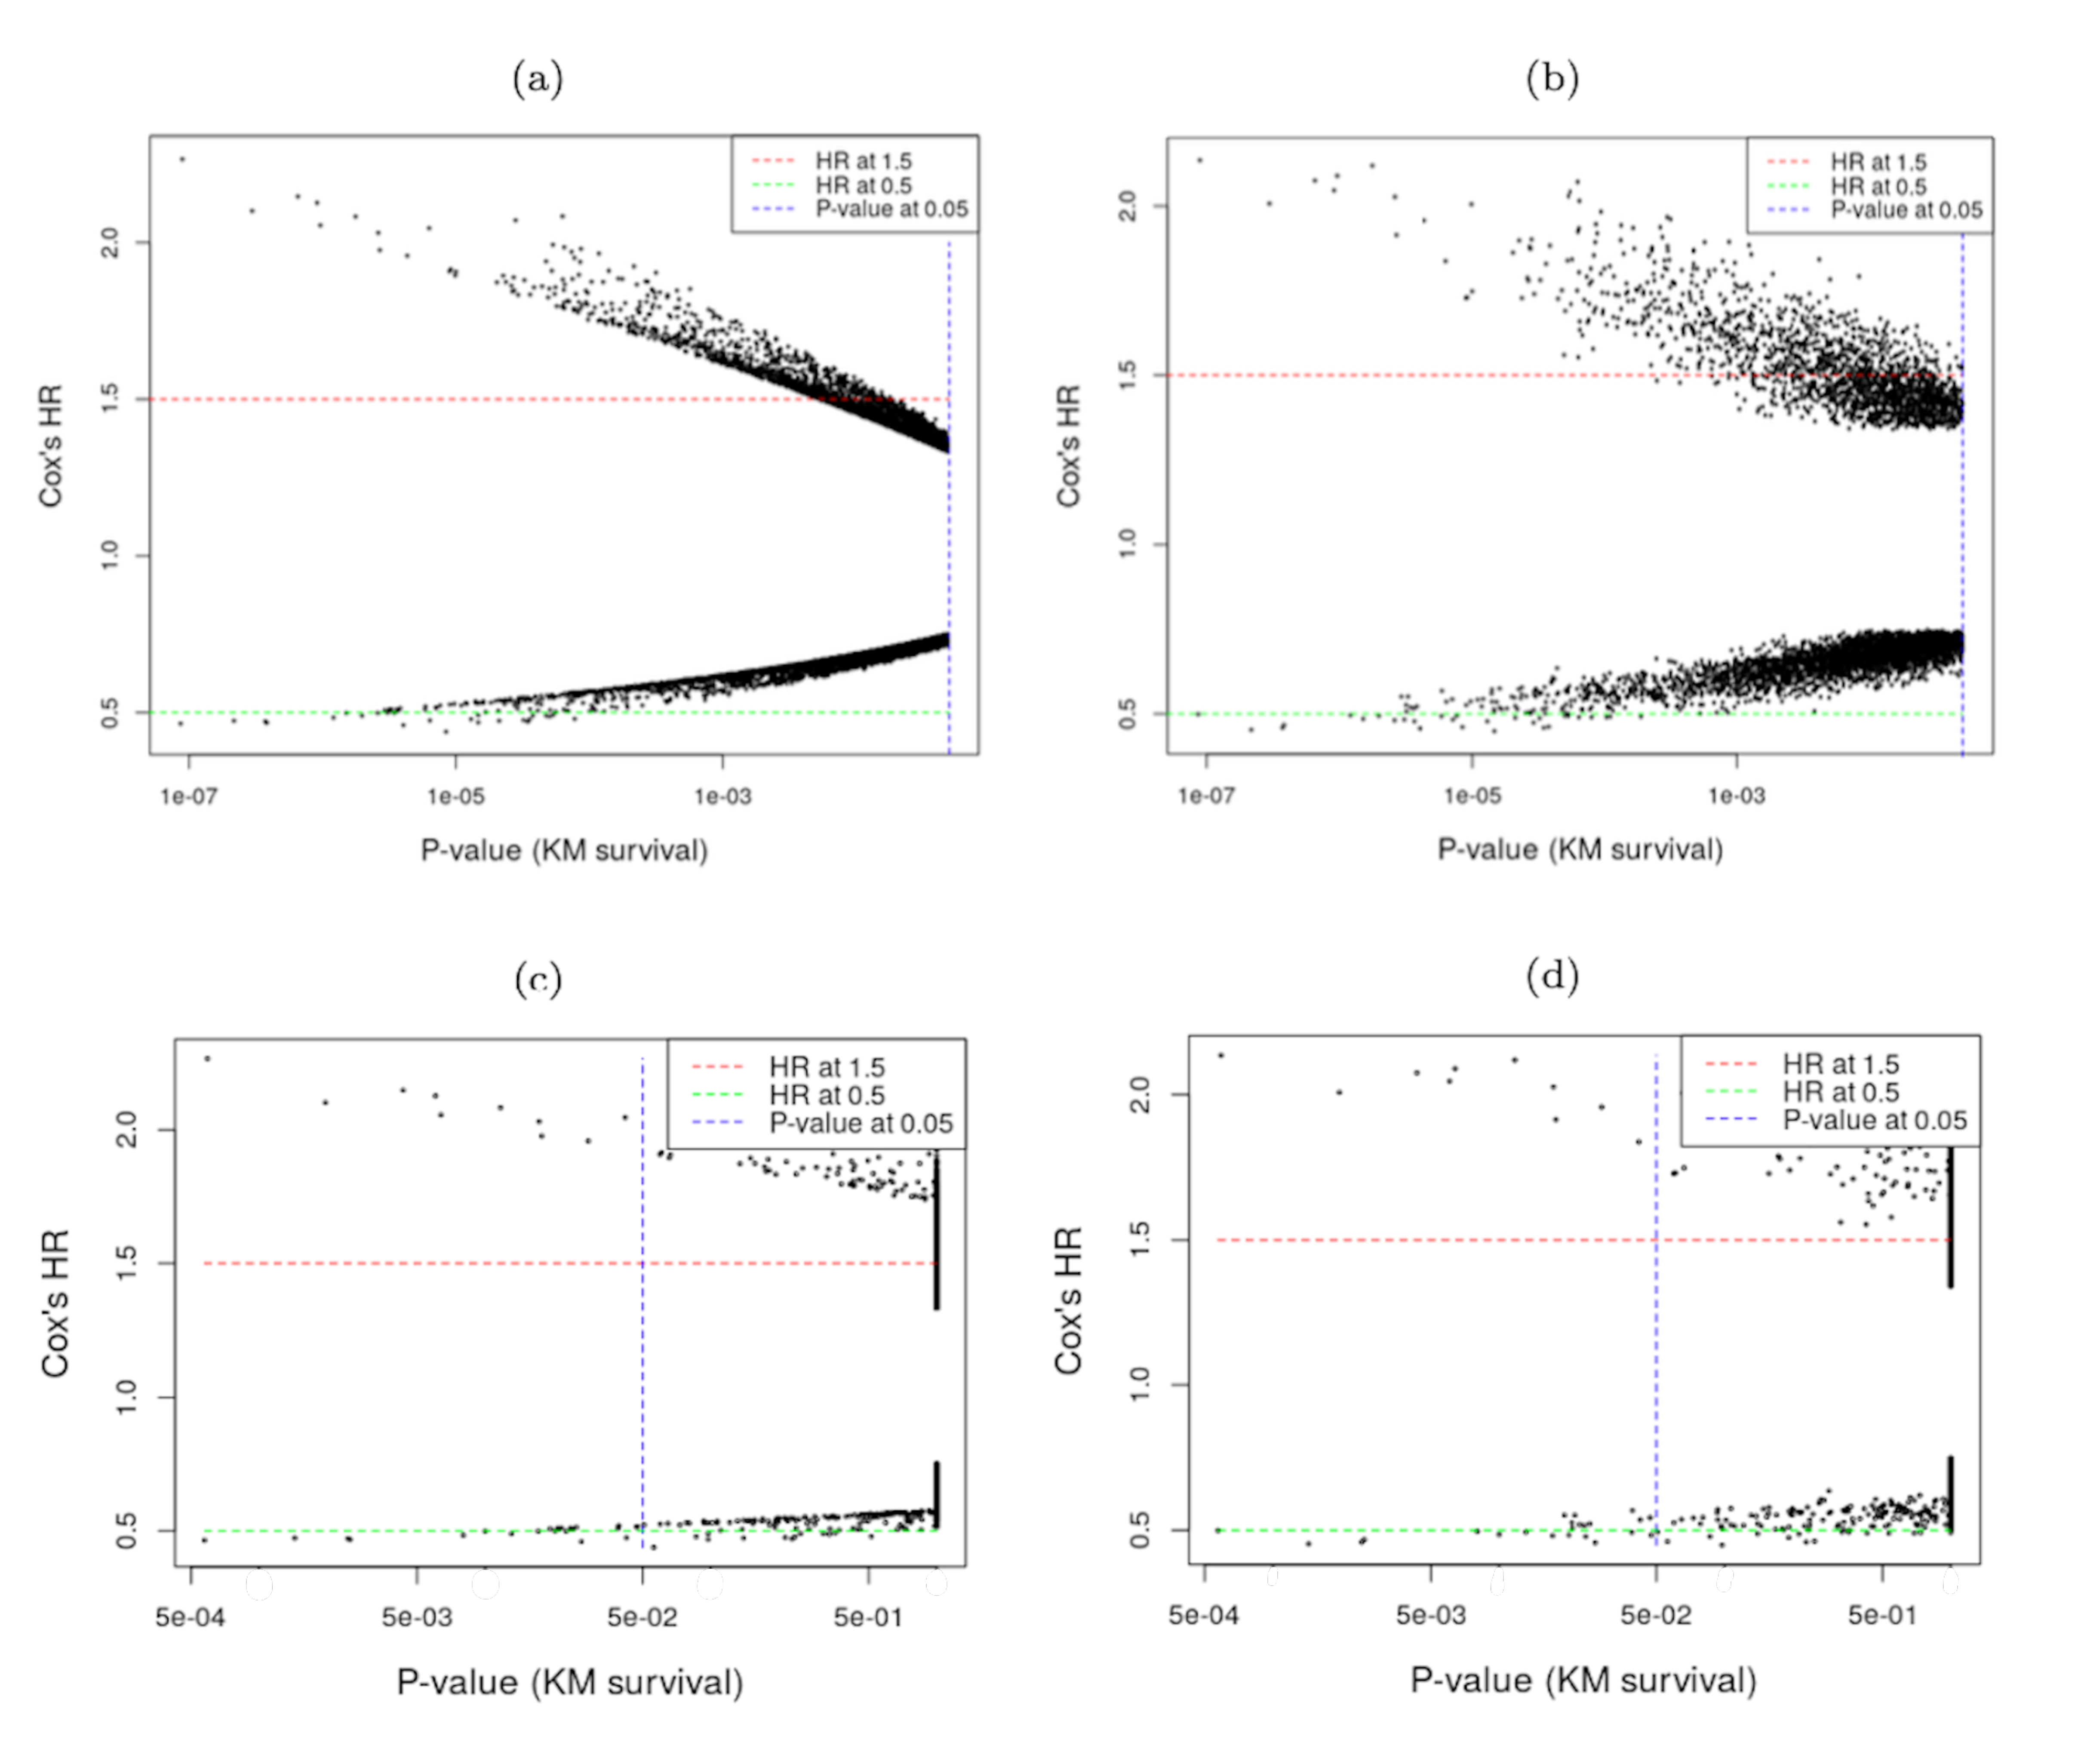
\includegraphics[width=14cm]{Figure2.pdf}
%\bcaption{\acrshort{hnscc} Cox's hazard ratio and \textit{P} value plot.}
%{(a) Univariate HR versus uncorrected \textit{P} value; (b) Multivariate HR versus uncorrected \textit{P} value; (c) Univariate HR versus Bonferroni corrected \textit{P} value; and (d) Multivariate HR versus Bonferroni corrected \textit{P} value.}
\label{fig:figure2}
\end{figure}

% tables 1  3
%%% tables
% Table1
% wide table \usepackage{tabularx}
% makecell{}






%\subsubsection{Figure 3:h}
\begin{figure}[hp]
\centering
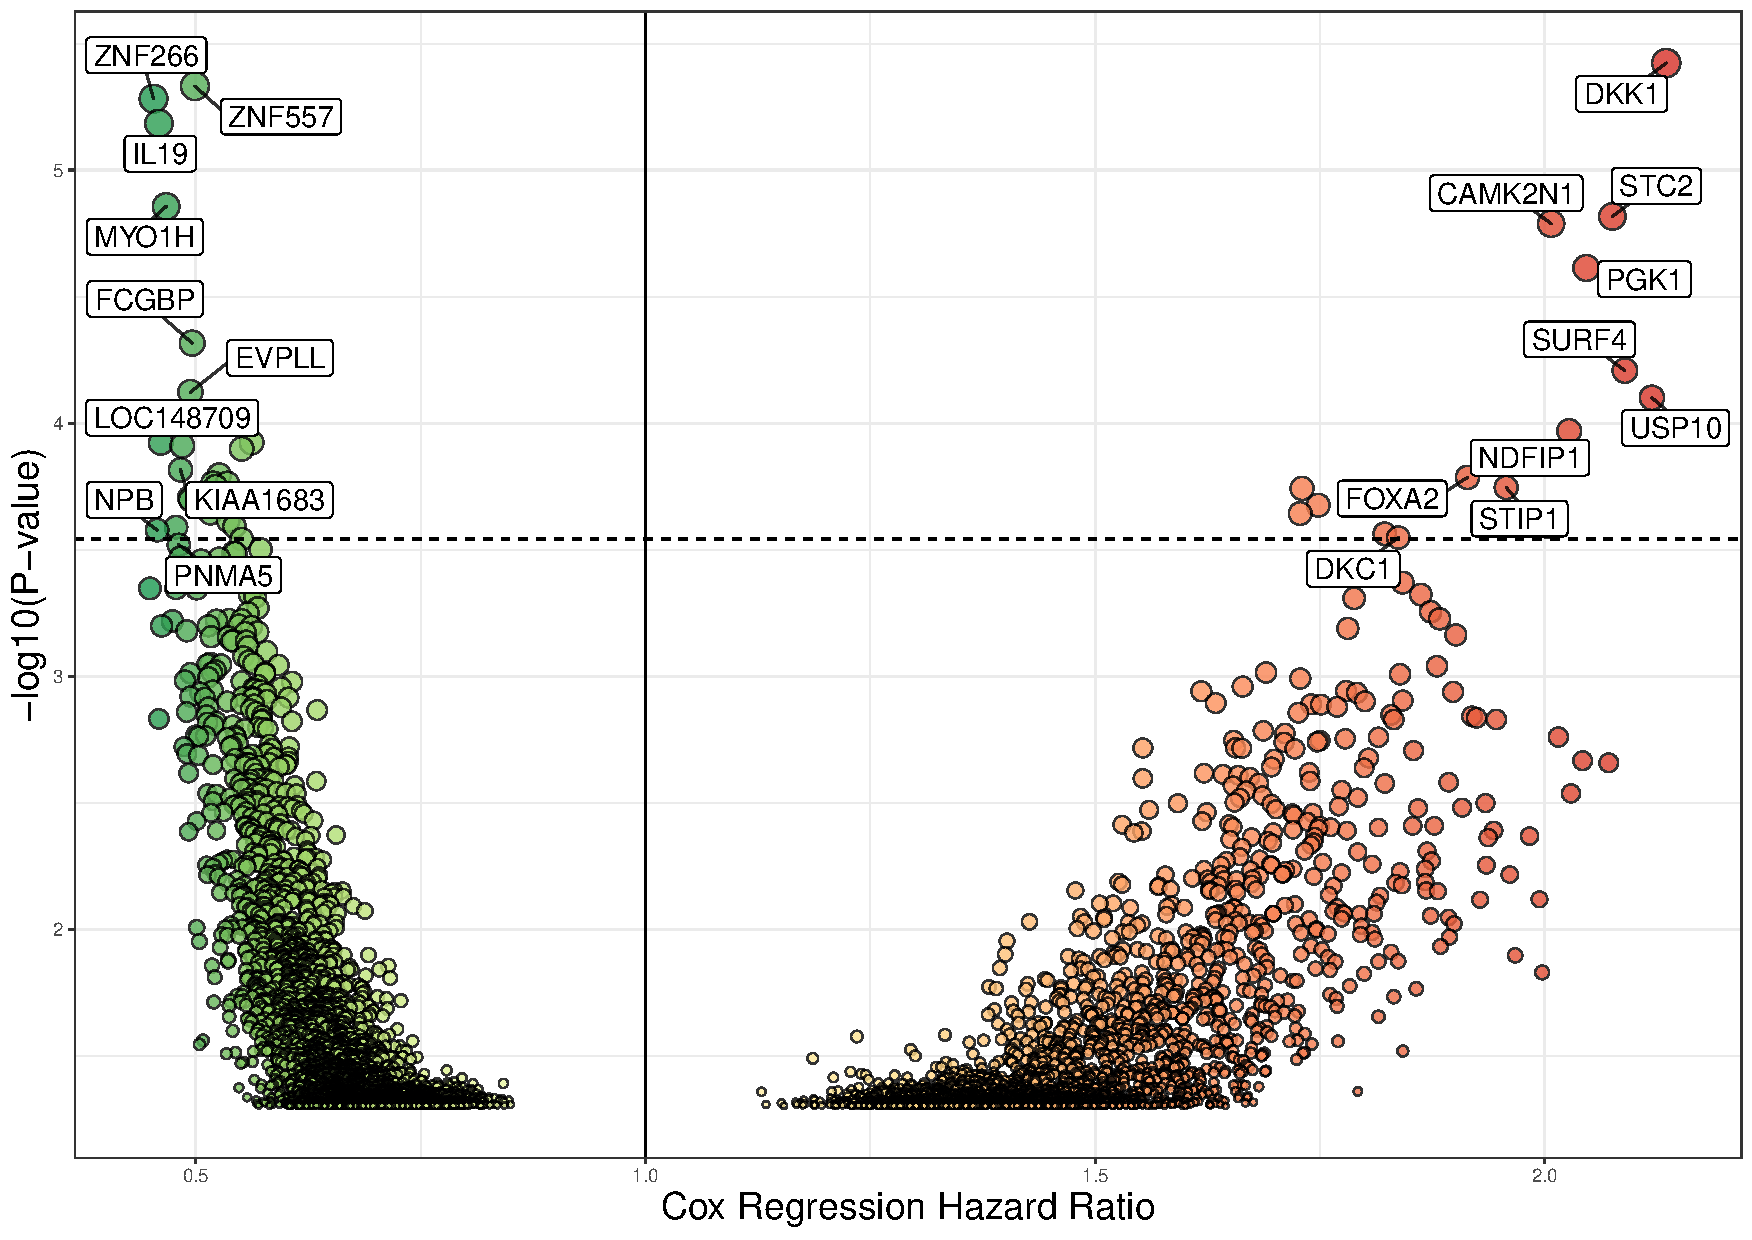
\includegraphics[width=14cm]{TCGA_HNSC_Optimal_Overall_allPlot_unKM_P_multiHR-Figure3.pdf} % .png from PvalueplotKM_20genes_Bonf.pdf
\bcaption{Volcano plot of genes under survival analyses.}
{X axis: unadjusted \textit{P} value of Kaplan-Meier survival (-log10 transformed).
Y axis: multivariate hazard ratio from Cox proportional regression model.
Dotted line: significant Bonferroni corrected \textit{P} value. 
\textcolor{red}{Red dots} mark 10 genes (unvalidated), which impact on poor prognosis ($HR>=1.5$). \textcolor{green}{Green dots} mark 10 genes (unvalidated), which affect on better survival ($HR<=0.5$).}
\label{fig:figure3}
\end{figure}
% new figure of volcano plot: TCGA_HNSC_Optimal_Overall_allPlot_unKM_P_multiHR.pdf, -log10(raw KM P-value) vs Cox multivariate HR
% X axis: "frequency" (number of uncorrected P-values less than 0.05 during Kaplan-Meier cutoff finding procedure). X axis: adjusted Kaplan-Meier P-value.

\clearpage


After validated by GSE2837, our top 1 candidate is \acrfull{CAMK2N1}. The Kaplan-Meier curve reveals 152 patients bearing the higher expression of \acrshort{CAMK2N1} were suffered from only 35\% of 5-year \acrshort{os} rate. In comparison, the other 262 patients with lower expression (the cutoff at 0.027(RSEM)) had a better prognosis (adjusted \textit{P} = $0.002$) (see Figure \ref{fig:figure4}(a)).
Figure \ref{fig:figure4}(b)'s cumulative \textit{P} value plot shows that the uncorrected 147 \textit{P} values ($< 0.05$) have been estimated by a serial cut from 144 to 290 persons for grouping the cohort in our cutoff finding procedure (cutofFinder\_func.R, see Figure \ref{fig:figure1}, cutoff engine). The smallest \textit{P} value (\num{2.97e-7}), when cut on n=262 (63.3\% of 414), has been defined as an optimal \textit{P} value.
Conversely, the most associated gene with better survival is \acrfull{IL19}. In Figure \ref{fig:figure4}(c), a Kaplan-Meier curve reveals 215 patients bearing the higher expression of \acrshort{IL19} had 60\% of 5-year OS survival rate (adjusted \textit{P} = $0.002$). The cutoff finding procedure (cutofFinder\_func.R) generated cumulative \textit{P} value plot in Figure \ref{fig:figure4}(d). The 161 uncorrected \textit{P} values were estimated by a serial cut from 125 to 286 for grouping the cohort. The smallest \textit{P} value (\num{3.73e-7}), when cut on n=199 (48.1\% of total cohort 414), has been defined as an optimal \textit{P} value with a cutoff value -0.147(RSEM) of \acrshort{rnaseq}.
%The second candidate, which improving patient survival, is ZNF266.
%\subsubsection{Tables} in main article

%\subsubsection{Figure 4:h}
\begin{figure}[hp]
\centering
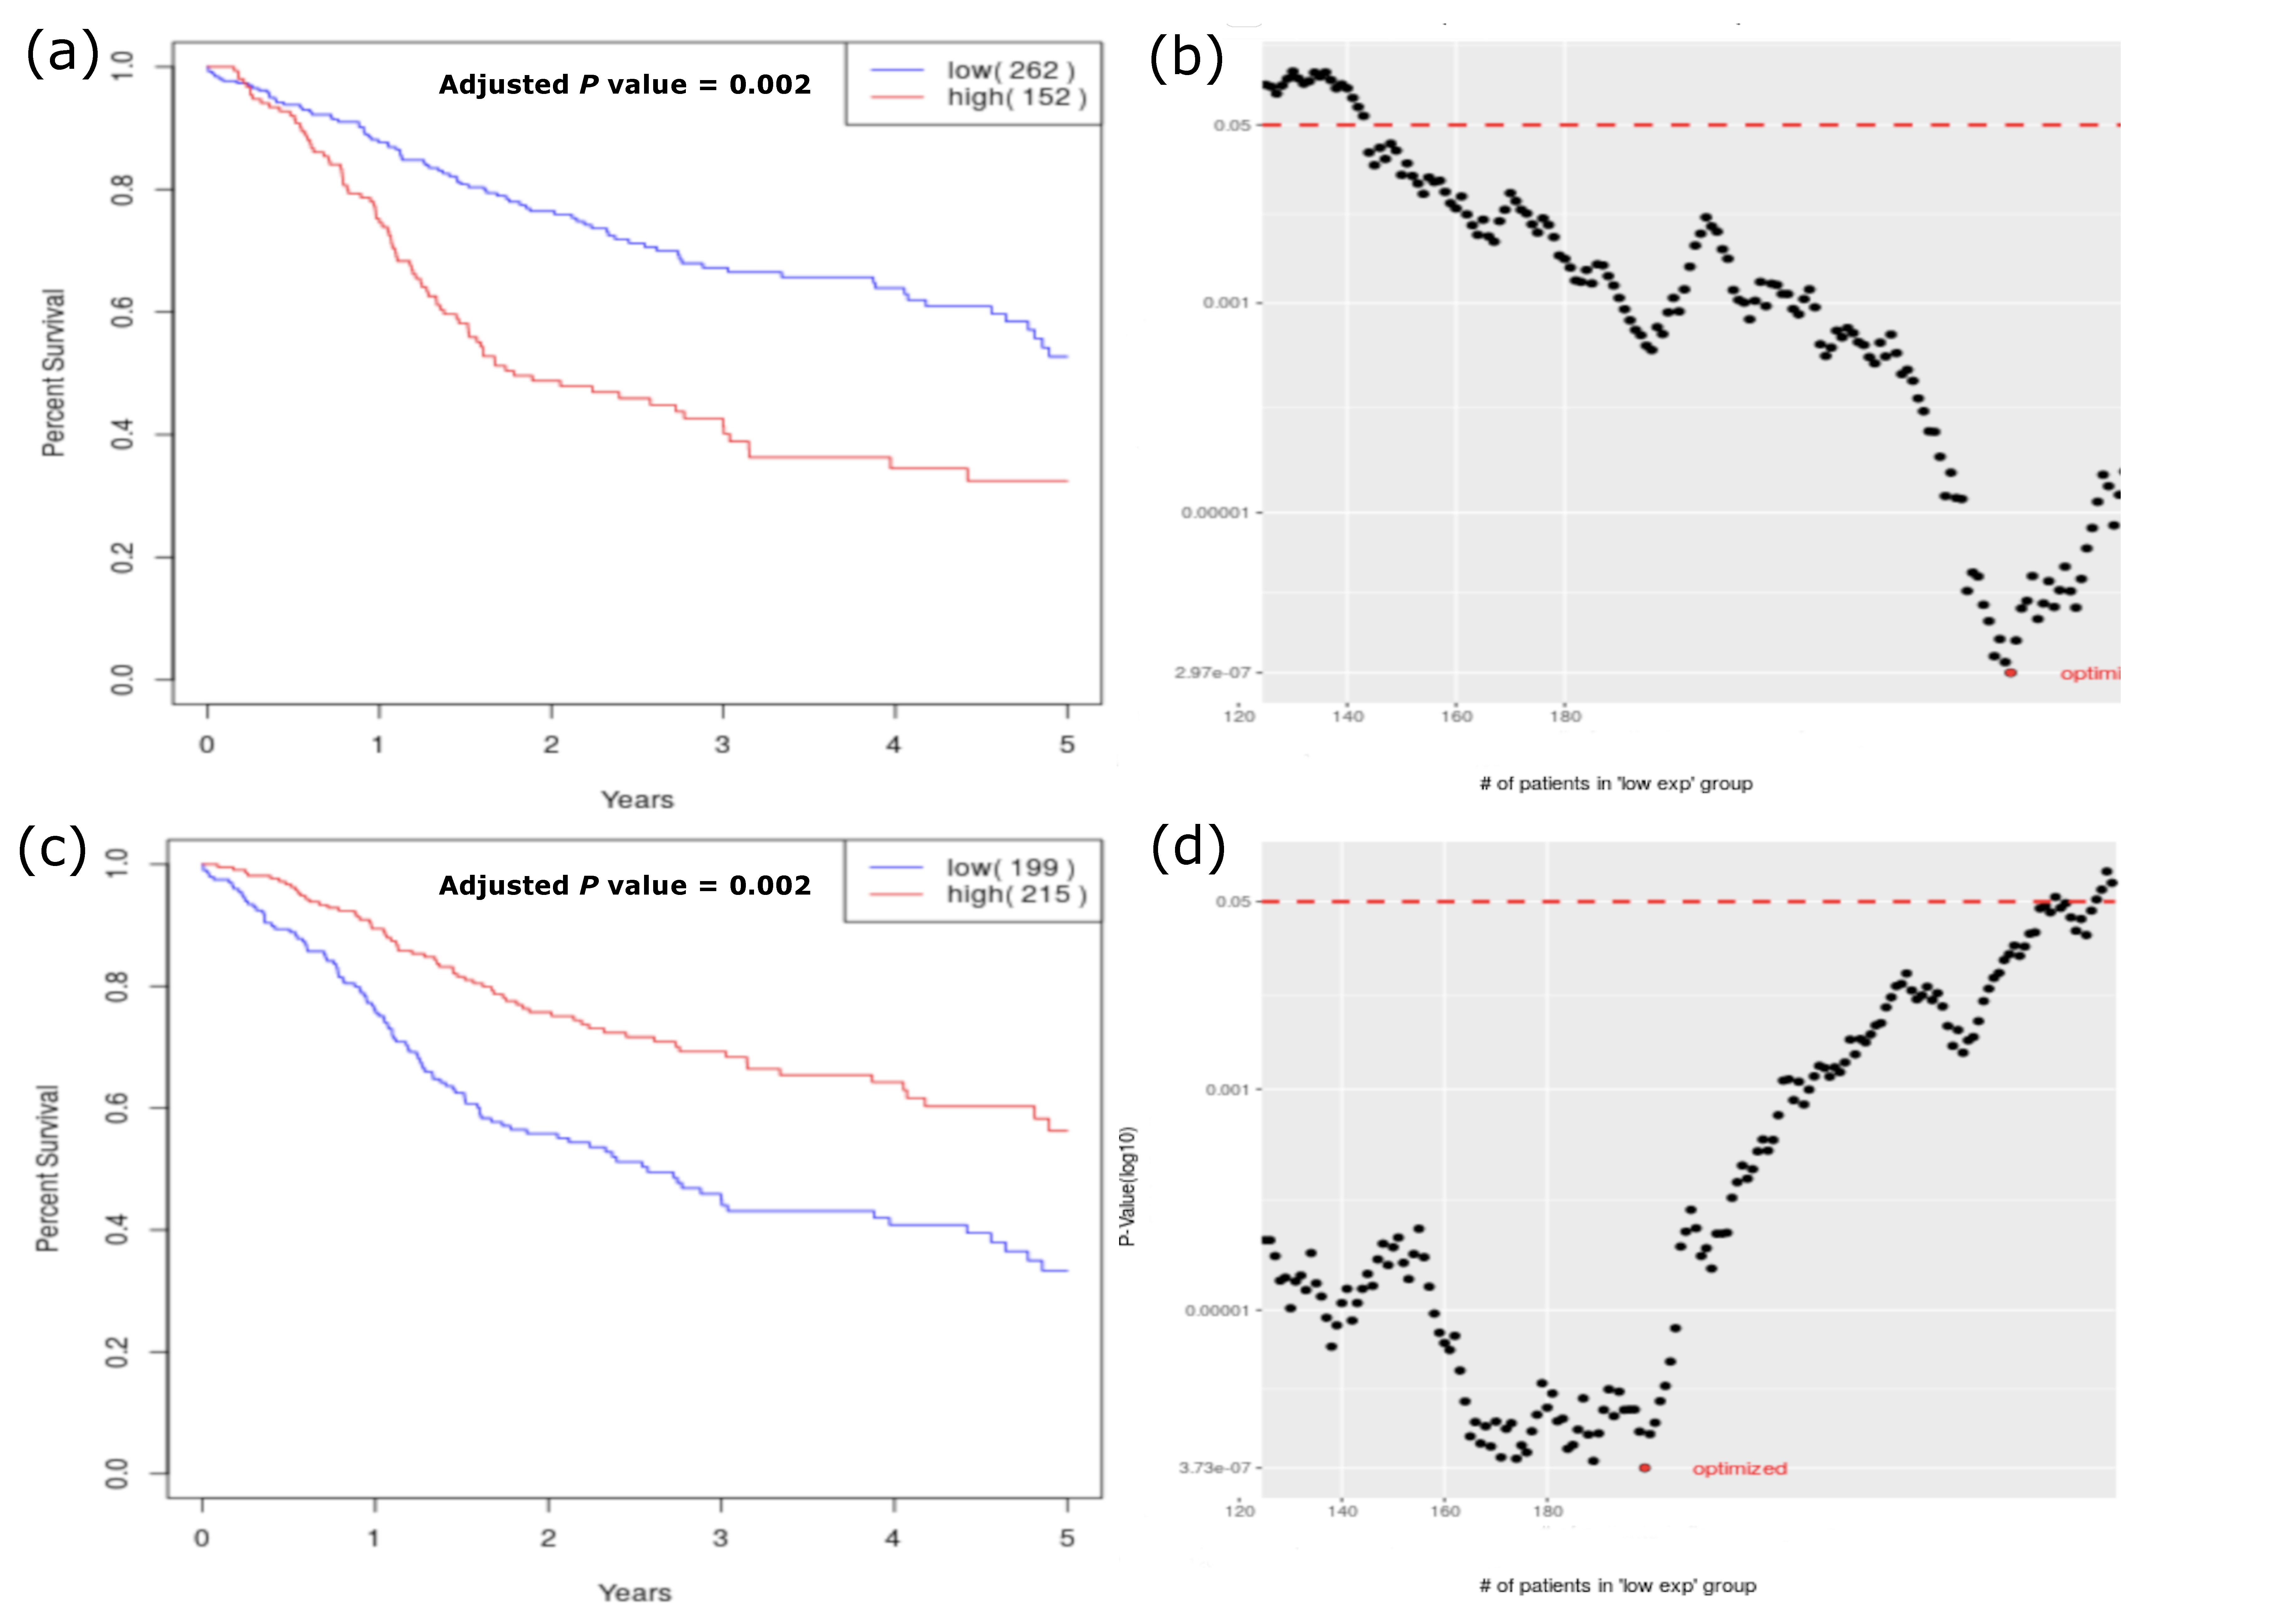
\includegraphics[width=15cm]{Figure_4_CAMK2N1_IL19.pdf}
\bcaption{Kaplan-Meier survival analyses, by cutoff finding.}
{(a) Kaplan-Meier plot of CAMK2N1 under optimal \textit{P} value, and (b) the cutoff is derived from cumulative \textit{P} value plot of CAMK2N1. (c) Kaplan-Meier plot of IL19 under optimal \textit{P} value, and (d) the cutoff is derived from cumulative \textit{P} value plot of IL19.}
\label{fig:figure4}
\end{figure}

\clearpage

%Table \ref{table:table1} shows ten overexpressed genes are associated with poor prognosis in \acrshort{hnscc}, ranked by adjusted Kaplan-Meier \textit{P} value.
Six out of ten preliminary candidates has been validated by using GSE2837.
We found those six candidates have the Cox's univariate and multivariate HR above 1.914.
%There were few published articles of \acrfull{SURF4} and \acrfull{NDFIP1} (\acrshort{NEDD4}: \acrlong{NEDD4}), which were related to cancer research.
In Table \ref{table:table2}, % table 3
after adjustment of confounders, \acrshort{CAMK2N1} overexpression is the independent prognostic factor (multivariate HR 2.007 [95\% CI: 1.490-2.704, \textit{P} $<$ 0.001]), as well as clinical T stage (HR 1.982 [95\% CI: 1.048-3.745, \textit{P} = 0.035]) and surgical margins status (HR 1.631 [95\% CI: 1.182-2.250, \textit{P} = 0.003]). 
Older age (more than 65) also worse the survival (HR 1.391 [95\% CI: 1.025-1.888, \textit{P} = 0.034]). 
The M stage could be ignored in this cohort due to only 3 out of 414 patients with distant metastasis.






%\subsubsection{Table3/legend} Table 3
%Table 2. Univariate/Multivariate Cox's proportional hazards regression analyses on OS time of DKK1 gene expression in HNSCC.
%(P-value Significant codes is denoted as  0.01 mark as *; 0.001 mark as **; if $<$0.001  mark as ***)
\begin{table}[hp]
\centering
\caption{Univariate/multivariate Cox's proportional hazards regression analyses on OS time of CAMK2N1 gene expression in HNSCC}
\arrayrulecolor[rgb]{0.255,0.255,0.255}
\resizebox{\linewidth}{!}{%
\begin{tabular}{|l|l|l|l|l|l|l|l|} 
%\begin{tabularx}{\textwidth}{|p{2.5cm}|l|l|l|l|l|l|l|} 
\arrayrulecolor{black}\cline{1-2}\arrayrulecolor[rgb]{0.255,0.255,0.255}\cline{3-8}
\multicolumn{2}{|l!{\color{black}\vrule}}{\multirow{2}{*}{Features}}                                                          & \multicolumn{3}{c|}{Univariate}                                                                                                                                                                                                                & \multicolumn{3}{c|}{Multivariate}                                                                                                                                                                                                               \\ 
\cline{3-8}
\multicolumn{2}{|l!{\color{black}\vrule}}{}                                                                                   & \multicolumn{1}{l!{\color{black}\vrule}}{HR}                                   & \multicolumn{1}{c!{\color{black}\vrule}}{CI95\%}                              & \multicolumn{1}{l!{\color{black}\vrule}}{\textit{P}~value}                    & \multicolumn{1}{l!{\color{black}\vrule}}{HR}                                   & \multicolumn{1}{c!{\color{black}\vrule}}{CI95\%}                              & \multicolumn{1}{l!{\color{black}\vrule}}{\textit{P}~value}                     \\ 
\arrayrulecolor{black}\hline
\multirow{2}{*}{Gender}                 & \multicolumn{1}{l!{\color{black}\vrule}}{{\cellcolor[rgb]{0.62,0.812,0.878}}Female} & \multicolumn{1}{l!{\color{black}\vrule}}{{\cellcolor[rgb]{0.62,0.812,0.878}}1} & \multicolumn{1}{l!{\color{black}\vrule}}{{\cellcolor[rgb]{0.62,0.812,0.878}}} & \multicolumn{1}{l!{\color{black}\vrule}}{{\cellcolor[rgb]{0.62,0.812,0.878}}} & \multicolumn{1}{l!{\color{black}\vrule}}{{\cellcolor[rgb]{0.62,0.812,0.878}}1} & \multicolumn{1}{l!{\color{black}\vrule}}{{\cellcolor[rgb]{0.62,0.812,0.878}}} & \multicolumn{1}{l!{\color{black}\vrule}}{{\cellcolor[rgb]{0.62,0.812,0.878}}}  \\ 
\cline{2-8}
                                        & Male                                                                                & 1.157                                                                          & 0.843-1.587                                                                   & 0.367                                                                         & 1.076                                                                          & 0.767-1.510                                                                   & 0.671                                                                          \\ 
\arrayrulecolor[rgb]{0.255,0.255,0.255}\hline
\multirow{2}{*}{Age at diagnosis}       & {\cellcolor[rgb]{0.62,0.812,0.878}}=65y                                             & {\cellcolor[rgb]{0.62,0.812,0.878}}1                                           & {\cellcolor[rgb]{0.62,0.812,0.878}}                                           & {\cellcolor[rgb]{0.62,0.812,0.878}}                                           & {\cellcolor[rgb]{0.62,0.812,0.878}}1                                           & {\cellcolor[rgb]{0.62,0.812,0.878}}                                           & {\cellcolor[rgb]{0.62,0.812,0.878}}                                            \\ 
\cline{2-8}
                                        & 65y                                                                                 & 1.329                                                                          & 0.990-1.784                                                                   & 0.058                                                                         & 1.391                                                                          & 1.025-1.888                                                                   & \textcolor{red}{0.034}                                                         \\ 
\hline
\multirow{2}{*}{Clinical T Status}      & {\cellcolor[rgb]{0.62,0.812,0.878}}T1+T2                                            & {\cellcolor[rgb]{0.62,0.812,0.878}}1                                           & {\cellcolor[rgb]{0.62,0.812,0.878}}                                           & {\cellcolor[rgb]{0.62,0.812,0.878}}                                           & {\cellcolor[rgb]{0.62,0.812,0.878}}1                                           & {\cellcolor[rgb]{0.62,0.812,0.878}}                                           & {\cellcolor[rgb]{0.62,0.812,0.878}}                                            \\ 
\cline{2-8}
                                        & T3+T4                                                                               & 1.409                                                                          & 1.028-1.931                                                                   & \textcolor{red}{0.033}                                                        & 1.982                                                                          & 1.048-3.745                                                                   & \textcolor{red}{0.035}                                                         \\ 
\hline
\multirow{2}{*}{Clinical N Status}      & {\cellcolor[rgb]{0.62,0.812,0.878}}N0                                               & {\cellcolor[rgb]{0.62,0.812,0.878}}1                                           & {\cellcolor[rgb]{0.62,0.812,0.878}}                                           & {\cellcolor[rgb]{0.62,0.812,0.878}}                                           & {\cellcolor[rgb]{0.62,0.812,0.878}}1                                           & {\cellcolor[rgb]{0.62,0.812,0.878}}                                           & {\cellcolor[rgb]{0.62,0.812,0.878}}                                            \\ 
\cline{2-8}
                                        & N1-3                                                                                & 1.185                                                                          & 0.890-1.577                                                                   & 0.246                                                                         & 1.145                                                                          & 0.801-1.636                                                                   & 0.457                                                                          \\ 
\hline
\multirow{2}{*}{Clinical M Status}      & {\cellcolor[rgb]{0.62,0.812,0.878}}M0                                               & {\cellcolor[rgb]{0.62,0.812,0.878}}1                                           & {\cellcolor[rgb]{0.62,0.812,0.878}}                                           & {\cellcolor[rgb]{0.62,0.812,0.878}}                                           & {\cellcolor[rgb]{0.62,0.812,0.878}}1                                           & {\cellcolor[rgb]{0.62,0.812,0.878}}                                           & {\cellcolor[rgb]{0.62,0.812,0.878}}                                            \\ 
\cline{2-8}
                                        & M1                                                                                  & 4.097                                                                          & 1.009-16.644                                                                  & \textcolor{red}{0.049}                                                        & 7.314                                                                          & 1.590-33.631                                                                  & \textcolor{red}{0.011}                                                         \\ 
\hline
\multirow{2}{*}{Clinical Stage}         & {\cellcolor[rgb]{0.62,0.812,0.878}}Stage I+II                                       & {\cellcolor[rgb]{0.62,0.812,0.878}}1                                           & {\cellcolor[rgb]{0.62,0.812,0.878}}                                           & {\cellcolor[rgb]{0.62,0.812,0.878}}                                           & {\cellcolor[rgb]{0.62,0.812,0.878}}1                                           & {\cellcolor[rgb]{0.62,0.812,0.878}}                                           & {\cellcolor[rgb]{0.62,0.812,0.878}}                                            \\ 
\cline{2-8}
                                        & Stage III+IV                                                                        & 1.245                                                                          & 0.882-1.759                                                                   & 0.213                                                                         & 0.621                                                                          & 0.287-1.343                                                                   & 0.226                                                                          \\ 
\hline
\multirow{2}{*}{Surgical Margin status} & {\cellcolor[rgb]{0.62,0.812,0.878}}Negative                                         & {\cellcolor[rgb]{0.62,0.812,0.878}}1                                           & {\cellcolor[rgb]{0.62,0.812,0.878}}                                           & {\cellcolor[rgb]{0.62,0.812,0.878}}                                           & {\cellcolor[rgb]{0.62,0.812,0.878}}1                                           & {\cellcolor[rgb]{0.62,0.812,0.878}}                                           & {\cellcolor[rgb]{0.62,0.812,0.878}}                                            \\ 
\cline{2-8}
                                        & Positive                                                                            & 1.591                                                                          & 1.155–2.191                                                                   & \textcolor{red}{0.004}                                                        & 1.631                                                                          & 1.182-2.250                                                                   & \textcolor{red}{0.003}                                                         \\ 
\hline
\multirow{2}{*}{Tobacco Exposure}       & {\cellcolor[rgb]{0.62,0.812,0.878}}Low                                              & {\cellcolor[rgb]{0.62,0.812,0.878}}1                                           & {\cellcolor[rgb]{0.62,0.812,0.878}}                                           & {\cellcolor[rgb]{0.62,0.812,0.878}}                                           & {\cellcolor[rgb]{0.62,0.812,0.878}}1                                           & {\cellcolor[rgb]{0.62,0.812,0.878}}                                           & {\cellcolor[rgb]{0.62,0.812,0.878}}                                            \\ 
\cline{2-8}
                                        & High                                                                                & 1.364                                                                          & 1.008-1.844                                                                   & \textcolor{red}{0.044}                                                        & 1.363                                                                          & 0.990-1.875                                                                   & 0.058                                                                          \\ 
\hline
\multirow{2}{*}{RNA-Seq}                & {\cellcolor[rgb]{0.62,0.812,0.878}}Low                                              & {\cellcolor[rgb]{0.62,0.812,0.878}}1                                           & {\cellcolor[rgb]{0.62,0.812,0.878}}                                           & {\cellcolor[rgb]{0.62,0.812,0.878}}                                           & {\cellcolor[rgb]{0.62,0.812,0.878}}1                                           & {\cellcolor[rgb]{0.62,0.812,0.878}}                                           & {\cellcolor[rgb]{0.62,0.812,0.878}}                                            \\ 
\cline{2-8}
                                        & High                                                                                & 2.101                                                                          & 1.572-2.809                                                                   & \multicolumn{1}{c|}{\textcolor{red}{***}}                                     & 2.007                                                                          & 1.490-2.704                                                                   & \multicolumn{1}{c|}{\textcolor{red}{***}}                                      \\ 
\hline
\multicolumn{8}{|l|}{}                                                                                                                                                                                                                                                                                                                                                                                                                                                                                                                                                                                                           \\ 
\hline
\multicolumn{8}{|l|}{(\textit{P}~value significant codes is denoted: red \textless{} 0.05; *** \textless{} 0.001)}                                                                                                                                                                                                                                                                                                                                                                                                                                                                                                               \\
\hline
\end{tabular}
} % end of \resizebox
\arrayrulecolor{black}
\label{table:table2}
\end{table}




%In Table \ref{table:table3}, the other ten overexpressed genes have been found in better prognosis of \acrshort{hnscc} patients. Cox's univariate and multivariate HR is under 0.5.
%Four out of ten has been validated by using GSE2837.
In Table \ref{table:table4},
after adjustment of confounders, prognosis is influenced by advance clinical T Status (HR 1.961 [95\% CI: 1.035-3.714, \textit{P} = 0.039] ), positive surgical margin involvement (HR 1.631 [95\% CI: 1.18-2.254, \textit{P} = 0.003]) , and higher tobacco exposure (HR 1.453 [95\% CI: 1.055-2.000, \textit{P} = 0.022]).
Overexpressed \acrshort{IL19} gene could has a protective influencce on prognosis (HR 0.499 [95\% CI: 0.372-0.669, \textit{P} $<$ 0.001]).


In summary, those ten candidate biomarkers, clinical T stage, and surgical margin are independent prognosis factors in \acrshort{hnscc}.
Thus, the prognosis model with coefficients is established from \acrshort{tcga} \acrshort{hnscc} cohort. 
%The important input $X_1...X_n$ should be patients' features: age, specific ten gene expressions, clinical T stage, and surgical margin.
%\\[0.5cm]
% total 6+4 =10
% After validation with an independent \acrshort{hnscc} cohort (GSE2837), the result showed six overexpressed genes (symbol as CAMK2N1, PGK1, SURF4, USP10, NDFIP1, FOXA2) are significantly associated with a poor prognosis of overall survival. 
%Furthermore, the four overexpressed genes (symbol as IL19, FCGBP, IQCN - former symbol as KIAA1683, and NPB) are correlated with better survival.




%\subsubsection{Table4/legend} Table 4
\begin{table}[!hp]
\centering
\caption{Univariate/multivariate Cox's proportional hazards regression analyses on OS time of IL19 gene expression in HNSCC}
\arrayrulecolor[rgb]{0.255,0.255,0.255}
\resizebox{\linewidth}{!}{%
\begin{tabular}{|l|l|l|l|l|l!{\color{black}\vrule}l!{\color{black}\vrule}l!{\color{black}\vrule}} 
\arrayrulecolor{black}\cline{1-2}\arrayrulecolor[rgb]{0.255,0.255,0.255}\cline{3-8}
\multicolumn{2}{|l!{\color{black}\vrule}}{\multirow{2}{*}{Features}}                                                          & \multicolumn{3}{c|}{Univariate}                                                                                                                                                                                                                & \multicolumn{3}{c|}{Multivariate}                                                                                                    \\ 
\cline{3-8}
\multicolumn{2}{|l!{\color{black}\vrule}}{}                                                                                   & \multicolumn{1}{l!{\color{black}\vrule}}{HR}                                   & \multicolumn{1}{c!{\color{black}\vrule}}{CI95\%}                              & \multicolumn{1}{l!{\color{black}\vrule}}{\textit{P}~value}                    & HR                                   & \multicolumn{1}{c!{\color{black}\vrule}}{CI95\%} & \textit{P}~value                           \\ 
\arrayrulecolor{black}\hline
\multirow{2}{*}{Gender}                 & \multicolumn{1}{l!{\color{black}\vrule}}{{\cellcolor[rgb]{0.62,0.812,0.878}}Female} & \multicolumn{1}{l!{\color{black}\vrule}}{{\cellcolor[rgb]{0.62,0.812,0.878}}1} & \multicolumn{1}{l!{\color{black}\vrule}}{{\cellcolor[rgb]{0.62,0.812,0.878}}} & \multicolumn{1}{l!{\color{black}\vrule}}{{\cellcolor[rgb]{0.62,0.812,0.878}}} & {\cellcolor[rgb]{0.62,0.812,0.878}}1 & {\cellcolor[rgb]{0.62,0.812,0.878}}              & {\cellcolor[rgb]{0.62,0.812,0.878}}        \\ 
\cline{2-8}
                                        & Male                                                                                & 1.157                                                                          & 0.843-1.587                                                                   & 0.367                                                                         & 1.183                                & 0.847-1.652                                      & 0.325                                      \\ 
\hhline{>{\arrayrulecolor[rgb]{0.255,0.255,0.255}}|----->{\arrayrulecolor{black}}->{\arrayrulecolor{black}}->{\arrayrulecolor{black}}-|}
\multirow{2}{*}{Age at diagnosis}       & {\cellcolor[rgb]{0.62,0.812,0.878}}=65y                                             & {\cellcolor[rgb]{0.62,0.812,0.878}}1                                           & {\cellcolor[rgb]{0.62,0.812,0.878}}                                           & {\cellcolor[rgb]{0.62,0.812,0.878}}                                           & {\cellcolor[rgb]{0.62,0.812,0.878}}1 & {\cellcolor[rgb]{0.62,0.812,0.878}}              & {\cellcolor[rgb]{0.62,0.812,0.878}}        \\ 
\arrayrulecolor[rgb]{0.255,0.255,0.255}\cline{2-5}\arrayrulecolor{black}\cline{6-6}\arrayrulecolor{black}\cline{7-7}\arrayrulecolor{black}\cline{8-8}
                                        & 65y                                                                                 & 1.329                                                                          & 0.990-1.784                                                                   & 0.058                                                                         & 1.481                                & 1.087-2.018                                      & \textcolor{red}{0.013}                     \\ 
\hhline{>{\arrayrulecolor[rgb]{0.255,0.255,0.255}}|----->{\arrayrulecolor{black}}->{\arrayrulecolor{black}}->{\arrayrulecolor{black}}-|}
\multirow{2}{*}{Clinical T Status}      & {\cellcolor[rgb]{0.62,0.812,0.878}}T1+T2                                            & {\cellcolor[rgb]{0.62,0.812,0.878}}1                                           & {\cellcolor[rgb]{0.62,0.812,0.878}}                                           & {\cellcolor[rgb]{0.62,0.812,0.878}}                                           & {\cellcolor[rgb]{0.62,0.812,0.878}}1 & {\cellcolor[rgb]{0.62,0.812,0.878}}              & {\cellcolor[rgb]{0.62,0.812,0.878}}        \\ 
\arrayrulecolor[rgb]{0.255,0.255,0.255}\cline{2-5}\arrayrulecolor{black}\cline{6-6}\arrayrulecolor{black}\cline{7-7}\arrayrulecolor{black}\cline{8-8}
                                        & T3+T4                                                                               & 1.409                                                                          & 1.028-1.931                                                                   & \textcolor{red}{0.033}                                                        & 2.175                                & 1.152-4.106                                      & \textcolor{red}{0.017}                     \\ 
\hhline{>{\arrayrulecolor[rgb]{0.255,0.255,0.255}}|----->{\arrayrulecolor{black}}->{\arrayrulecolor{black}}->{\arrayrulecolor{black}}-|}
\multirow{2}{*}{Clinical N Status}      & {\cellcolor[rgb]{0.62,0.812,0.878}}N0                                               & {\cellcolor[rgb]{0.62,0.812,0.878}}1                                           & {\cellcolor[rgb]{0.62,0.812,0.878}}                                           & {\cellcolor[rgb]{0.62,0.812,0.878}}                                           & {\cellcolor[rgb]{0.62,0.812,0.878}}1 & {\cellcolor[rgb]{0.62,0.812,0.878}}              & {\cellcolor[rgb]{0.62,0.812,0.878}}        \\ 
\arrayrulecolor[rgb]{0.255,0.255,0.255}\cline{2-5}\arrayrulecolor{black}\cline{6-6}\arrayrulecolor{black}\cline{7-7}\arrayrulecolor{black}\cline{8-8}
                                        & N1-3                                                                                & 1.185                                                                          & 0.890-1.577                                                                   & 0.246                                                                         & 1.237                                & 0.864-1.770                                      & 0.245                                      \\ 
\hhline{>{\arrayrulecolor[rgb]{0.255,0.255,0.255}}|----->{\arrayrulecolor{black}}->{\arrayrulecolor{black}}->{\arrayrulecolor{black}}-|}
\multirow{2}{*}{Clinical M Status}      & {\cellcolor[rgb]{0.62,0.812,0.878}}M0                                               & {\cellcolor[rgb]{0.62,0.812,0.878}}1                                           & {\cellcolor[rgb]{0.62,0.812,0.878}}                                           & {\cellcolor[rgb]{0.62,0.812,0.878}}                                           & {\cellcolor[rgb]{0.62,0.812,0.878}}1 & {\cellcolor[rgb]{0.62,0.812,0.878}}              & {\cellcolor[rgb]{0.62,0.812,0.878}}        \\ 
\arrayrulecolor[rgb]{0.255,0.255,0.255}\cline{2-5}\arrayrulecolor{black}\cline{6-6}\arrayrulecolor{black}\cline{7-7}\arrayrulecolor{black}\cline{8-8}
                                        & M1                                                                                  & 4.097                                                                          & 1.009-16.644                                                                  & \textcolor{red}{0.049}                                                        & 8.629                                & 1.879-39.63                                      & \textcolor{red}{0.006}                     \\ 
\hhline{>{\arrayrulecolor[rgb]{0.255,0.255,0.255}}|----->{\arrayrulecolor{black}}->{\arrayrulecolor{black}}->{\arrayrulecolor{black}}-|}
\multirow{2}{*}{Clinical Stage}         & {\cellcolor[rgb]{0.62,0.812,0.878}}Stage I+II                                       & {\cellcolor[rgb]{0.62,0.812,0.878}}1                                           & {\cellcolor[rgb]{0.62,0.812,0.878}}                                           & {\cellcolor[rgb]{0.62,0.812,0.878}}                                           & {\cellcolor[rgb]{0.62,0.812,0.878}}1 & {\cellcolor[rgb]{0.62,0.812,0.878}}              & {\cellcolor[rgb]{0.62,0.812,0.878}}        \\ 
\arrayrulecolor[rgb]{0.255,0.255,0.255}\cline{2-5}\arrayrulecolor{black}\cline{6-6}\arrayrulecolor{black}\cline{7-7}\arrayrulecolor{black}\cline{8-8}
                                        & Stage III+IV                                                                        & 1.245                                                                          & 0.882-1.759                                                                   & 0.213                                                                         & 0.476                                & 0.222-1.024                                      & 0.057                                      \\ 
\hhline{>{\arrayrulecolor[rgb]{0.255,0.255,0.255}}|----->{\arrayrulecolor{black}}->{\arrayrulecolor{black}}->{\arrayrulecolor{black}}-|}
\multirow{2}{*}{Surgical Margin status} & {\cellcolor[rgb]{0.62,0.812,0.878}}Negative                                         & {\cellcolor[rgb]{0.62,0.812,0.878}}1                                           & {\cellcolor[rgb]{0.62,0.812,0.878}}                                           & {\cellcolor[rgb]{0.62,0.812,0.878}}                                           & {\cellcolor[rgb]{0.62,0.812,0.878}}1 & {\cellcolor[rgb]{0.62,0.812,0.878}}              & {\cellcolor[rgb]{0.62,0.812,0.878}}        \\ 
\arrayrulecolor[rgb]{0.255,0.255,0.255}\cline{2-5}\arrayrulecolor{black}\cline{6-6}\arrayrulecolor{black}\cline{7-7}\arrayrulecolor{black}\cline{8-8}
                                        & Positive                                                                            & 1.591                                                                          & 1.155–2.191                                                                   & \textcolor{red}{0.004}                                                        & 1.63                                 & 1.180-2.252                                      & \textcolor{red}{0.003}                     \\ 
\hhline{>{\arrayrulecolor[rgb]{0.255,0.255,0.255}}|----->{\arrayrulecolor{black}}->{\arrayrulecolor{black}}->{\arrayrulecolor{black}}-|}
\multirow{2}{*}{Tobacco Exposure}       & {\cellcolor[rgb]{0.62,0.812,0.878}}Low                                              & {\cellcolor[rgb]{0.62,0.812,0.878}}1                                           & {\cellcolor[rgb]{0.62,0.812,0.878}}                                           & {\cellcolor[rgb]{0.62,0.812,0.878}}                                           & {\cellcolor[rgb]{0.62,0.812,0.878}}1 & {\cellcolor[rgb]{0.62,0.812,0.878}}              & {\cellcolor[rgb]{0.62,0.812,0.878}}        \\ 
\arrayrulecolor[rgb]{0.255,0.255,0.255}\cline{2-5}\arrayrulecolor{black}\cline{6-6}\arrayrulecolor{black}\cline{7-7}\arrayrulecolor{black}\cline{8-8}
                                        & High                                                                                & 1.364                                                                          & 1.008-1.844                                                                   & \textcolor{red}{0.044}                                                        & 1.62                                 & 1.173-2.238                                      & \textcolor{red}{0.003}                     \\ 
\hhline{>{\arrayrulecolor[rgb]{0.255,0.255,0.255}}|----->{\arrayrulecolor{black}}->{\arrayrulecolor{black}}->{\arrayrulecolor{black}}-|}
\multirow{2}{*}{RNA-Seq}                & {\cellcolor[rgb]{0.62,0.812,0.878}}Low                                              & {\cellcolor[rgb]{0.62,0.812,0.878}}1                                           & {\cellcolor[rgb]{0.62,0.812,0.878}}                                           & {\cellcolor[rgb]{0.62,0.812,0.878}}                                           & {\cellcolor[rgb]{0.62,0.812,0.878}}1 & {\cellcolor[rgb]{0.62,0.812,0.878}}              & {\cellcolor[rgb]{0.62,0.812,0.878}}        \\ 
\arrayrulecolor[rgb]{0.255,0.255,0.255}\cline{2-5}\arrayrulecolor{black}\cline{6-6}\arrayrulecolor{black}\cline{7-7}\arrayrulecolor{black}\cline{8-8}
                                        & High                                                                                & 0.472                                                                          & 0.351-0.635                                                                   & \multicolumn{1}{c|}{\textcolor{red}{***}}                                     & \multicolumn{1}{l|}{0.459}           & 0.340-0.619                                      & \multicolumn{1}{c|}{\textcolor{red}{***}}  \\ 
\arrayrulecolor[rgb]{0.255,0.255,0.255}\cline{1-6}\arrayrulecolor{black}\cline{7-7}\arrayrulecolor[rgb]{0.255,0.255,0.255}\cline{8-8}
\multicolumn{8}{|l|}{}                                                                                                                                                                                                                                                                                                                                                                                                                                                                                                \\ 
\hline
\multicolumn{8}{|l|}{(\textit{P}~value significant codes is denoted: red \textless{} 0.05; *** \textless{} 0.001)}                                                                                                                                                                                                                                                                                                                                                                                                    \\
\hline
\end{tabular}
}% end of \resizebox
\arrayrulecolor{black}
\label{table:table4}
\end{table}



% end of result





%%%%%

%\section*{Figure}

\clearpage

\section{Deep Learning in Bioinformatics}

%why deep learning?
According to the recommendation of \acrfull{nci} (accessed at https://www.cancer.gov/\\research/areas/diagnosis/artificial-intelligence), 
\begin{outline}
\1 Artificial Intelligence (AI) is helpful to create opportunities in cancer research
\1 Image-based phenotype of cancer could be correlated with their underlying genomics data by deep learning methods
%Deep learning could predict commonly mutated genes and mRNA expression from the images
%\1 Aiding the genomics characterization of tumors by AI is crucial
\end{outline}

%== NCI deep learning could predict commonly mutated genes from the images:
Deep learning can be used to identify specific gene mutations and mRNA expression from tumor pathology images instead of using traditional genomic sequencing. 
For instance, NCI-funded researchers\citep{Coudray2018} at New York University used deep learning to analyze pathology images of lung tumors obtained from \acrfull{tcia}.
% Michael Snyder, Ph.D., chair of genetics at Stanford University, sees AI as the future of diagnosis. “I think we need to shift to using machine learning rather than rely on pathologists alone to do all the work,” he said. “Algorithms won’t replace pathologists, but they will assist them in making classifications. They will reduce the errors that pathologists would otherwise make.”
%The code developed for the project is available for other researchers to use for other diagnostic applications. The NYU team has already started applying the code to learn to diagnose kidney, breast, and other cancers.
The \acrshort{tcia} archives pathology images of tumor specimens available as a quality control measure for researchers studying the genetic sequence data collected in the \acrshort{tcga} project.
Coudray and his colleagues found that the deep learning method could accurately distinguish between lung adenocarcinoma and lung squamous cell carcinoma from the images\citep{Coudray2018}.
%how machine learning could help us?
% OFA:   The Cancer Imaging Archive (TCIA) whole-slide by Deep learning (ResNet)
%https://www.deeplearningbook.org/
%https://www.biorxiv.org/content/10.1101/2020.03.10.985887v1.full
%https://github.com/Serian1992/ImgBio.
%https://www.cancer.gov/research/areas/diagnosis/artificial-intelligence
Since a deep learning algorithm could potentially extract molecular phenotype from pathology images, 
mRNA expression could also be predicted from the images.
A HE2RNA model, developed by Schmauch and his colleagues\citep{Schmauch2020},  could predict RNA-Seq profiles from whole-slide images of \acrshort{tcia}. 
It has been validated by CD3- and CD20-\acrshort{ihc} staining. 
The transcriptomic representation learned by HE2RNA can also be transferred on other datasets.
%MKI67 is a well-known marker of cell proliferation, expressed both by tumor and adjacent normal cells, clinically determined by MIB1 or Ki67 IHC staining of whole-slide images. 
%  its surrounding cancerous area 
%Its overexpression around "surgical margin?" has been found to correlate with tumor growth, histological grade, and tumor recurrence.
% A high expression level of MKI67 is correlated with the most advanced stages of liver cancer.






\section{Conclusion}
High-throughput RNA-sequencing (RNA-Seq) is a powerful tool to characterize and quantify transcriptomes. Even the cost of RNA-Seq is continuously dropping, 
the budget of whole-genome transcriptomics study for survival analysis is still very high (USD350 to 500 per sample; 46 participants of HNSCC in TMU Joint Biobank, accessed on \today at http://ohr.tmu.edu.tw/front/jbb1/CaseNumber/pages.php?\\ID=dG11X29ociZDYXNlTnVtYmVy).
% NCI HE2RNA
By using the transcriptomic representation of RNA-Seq learned by NCI's HE2RNA project\citep{Schmauch2020},
%TCIA for whole-slide deep learning
we could validate and find more biomarkers from holistic \acrshort{ehr} and pathology images by the way of deep learning under R/Pytorch/Keras framework.


\clearpage



%%%%%%%%%%%%%%%%%

\section*{\cntext{(二)研究方法、進行步驟及執行進度}}
%1.本計畫採用之研究方法與原因。2.預計可能遭遇之困難及解決途徑 fallback approaches
% ***執行的策略
% 科技部鼓勵研究主題的系統性,也鼓勵具研究能力者從事較大型但 可能是較困難的長期研究。在建立研究架構的同時,要審慎考慮如何適當分配 每一年的執行進度。例如,容易有具體成果的部分可能要先放在前面作為基 礎,較困難的部分便可以逐年按部就班地進行調查分析。


\begin{outline}

Specific Aims %特定研究目標 (specific aims), 執行策略不能互相綁在一起, go paralleling, and equally balanced
\1 Aim 1: Construct a Deep Learning Platform of TCGA/TCIA and TMU dataset\\
%Survival Analysis\\
\1 Aim 2: Construct a Deep Learning Platform of Survival Analysis with EHR\\
\1 Aim 3: Biomarkers Discovery from RNA-Seq, Whole-slide Images, and EHR from TMU dataset\\

\end{outline}

\subsection{\cntext{執行進度}} % Flow Chart => Gantt chart
% A flowchart of a TeX workflow
% Author: Stefan Kottwitz
% https://www.packtpub.com/hardware-and-creative/latex-cookbook
%https://www.overleaf.com/project/60a23af9c83411b0f9067470
% https://texdoc.org/serve/smartdiagram/0
%\begin{document}



% A simpler example from the package documentation:
%
%\begin{ganttchart}{1}{12}
%  \gantttitle{2021}{12} \\
%  \gantttitlelist{1,...,12}{1} \\
%  \ganttgroup{Group 1}{1}{7} \\
%  \ganttbar{Task 1}{1}{2} \\
%  \ganttlinkedbar{Task 2}{3}{7} \ganttnewline
%  \ganttmilestone{Milestone}{7} \ganttnewline
%  \ganttbar{Final Task}{8}{12}
%  \ganttlink{elem2}{elem3}
%  \ganttlink{elem3}{elem4}
%\end{ganttchart}


\begin{ganttchart}[
    bar label node/.style={text width=5cm,align=right,font=\scriptsize\RaggedLeft,anchor=east},
    x unit=0.8cm,
    y unit title=0.4cm,
    y unit chart=0.6cm, %0.5
    vgrid,
    time slot format=isodate-yearmonth, %compress calendar,
    time slot unit=month,
    title/.append style={draw=none, fill=barblue},
    title label font=\sffamily\bfseries\color{white},
    title label node/.append style={below=-1.6ex},
    title left shift=.05,
    title right shift=-.05,
    title height=1,
    bar/.append style={draw=none, fill=groupblue},
    bar height=.6,
    bar label font=\normalsize\color{black!50},
    group right shift=0,
    group top shift=.6,
    group height=.3,
    group peaks height=.2,
    bar incomplete/.append style={fill=green}
   ]{2021-04}{2022-06}
   
   \gantttitlecalendar{year, month}\\ %=name
   \ganttbar[
    progress=100,
    bar progress label font=\small\color{barblue},
    bar progress label node/.append style={right=4pt},
    bar label font=\normalsize\color{barblue},
    name=pp
   ]{Preliminary}{2021-04}{2021-06} \\ % name=pp
   
\ganttset{progress label text={}, link/.style={black, -to}}

\ganttgroup{Aim 1}{2021-07}{2021-12} \\
\ganttbar[progress=4, name=T1A]{Solver Analysis $\&$ Formulation}{2021-07}{2021-10} \\
\ganttlinkedbar[progress=0]{Development of source code}{2021-10}{2021-12} \\

\ganttgroup{Aim 2}{2021-07}{2021-12} \\
\ganttbar[progress=15, name=T2A]{Solver Analysis $\&$ Formulation}{2021-07}{2021-10} \\
\ganttlinkedbar[progress=0]{Development of source code}{2021-10}{2021-12} \\

\ganttgroup{Aim 3}{2021-09}{2022-06} \\
  \ganttbar[progress=0]{Analysis of Experimental Data $\&$ Validation}{2021-09}{2022-06}
  \ganttnewline
%\ganttgroup{Aim 4}{2021-12}{2022-06} \\ %[group top shift =2] to avoid vertically overlap of bars
%  \ganttbar[progress=0]{Analysis of Experimental Data $\&$ Validation}{2021-12}{2022-06}
  % , bar top shift =1.8
  \ganttset{link/.style={green}}
  \ganttlink[link mid=.4]{pp}{T1A}
  \ganttlink[link mid=.159]{pp}{T2A}
\end{ganttchart}


\clearpage

\subsection{\cntext{計畫主體內容}} 
%[proposal main body] %(計畫的主體內容)” 解釋每個 aim 要怎麼做,著重策略之邏輯性鋪陳,盡量使論述具有說服力。
%新創一個方法或技術平台,須要詳細交代步驟

%\begin{outline}
\subsubsection{Aim 1:} Construct a Deep Learning Platform of TCGA/TCIA and TMU dataset\\[0.5cm]
%\end{outline}
%central issue 1 with preliminary data (key data); fallback approaches %先以概要式的背景介紹破題,點出研究目標的重要性,然後用邏輯之陳述將如何達成目標的策略和方法講清楚。請務必注意:每個研究目標基本上需具備其獨立性 (Independence),但其重要性卻要在目標之間有所連結,且要能回應總體目標之研究顯著性
Our preliminary data (biomarker candidates) could be served as the bridge between the prognosis of patients and their pathological images of specimen.
We will develop a deep-learning-based data mining as well as a validation platform. It might incorporate whole-slide images of pathology of \acrshort{hnscc} from the Cancer Imaging Archive (TCIA) and from Joint Biobank of Taipei Medical University (TMU dataset).
There is 98 slides from 46 patients with HNSCC in TMU dataset.
***TMU Joint IRB approval
%  an independent dataset of 369 slides from 194 patients with LIHC43 from hospital Henri Mondor (Mondor dataset)
%RNA-Seq data of \acrfull{tcga} for survival analysis. 

%https://wiki.cancerimagingarchive.net/display/Public/TCGA-HNSC
%https://cancer.digitalslidearchive.org/#!/CDSA/hnsc/TCGA-BA-4076/TCGA-BA-4076-01A-01-BS1?slide=TCGA-BA-4076-01A-01-BS1.4aef481c-f634-4ffc-9fb3-609f59a8caf9.svs

NCI's GDC stores pathology SVS image.
An SVS file is a digital slide image file created by an Aperio ScanScope slide scanner.
The HNSCC images is available at https://github.com/texchi2/HE2RNA\_code/\\blob/master/gdc\_manifests/gdc\_manifest.2018-06-26\_diagnostic\_TCGA-HNSC.txt.
%https://portal.gdc.cancer.gov/image-viewer?caseId=b843df7e-db06-4d29-b00d-6a93effd9191&filters=%7B%22op%22%3A%22and%22%2C%22content%22%3A%5B%7B%22op%22%3A%22in%22%2C%22content%22%3A%7B%22field%22%3A%22cases.project.project_id%22%2C%22value%22%3A%5B%22TCGA-HNSC%22%5D%7D%7D%2C%7B%22op%22%3A%22in%22%2C%22content%22%3A%7B%22field%22%3A%22files.experimental_strategy%22%2C%22value%22%3A%5B%22Tissue%20Slide%22%5D%7D%7D%5D%7D&selectedId=45fffd2f-e282-4198-8c49-0247507ebb8a
% HE2RNA
%*** github: https://github.com/owkin/HE2RNA_code

%the ability of HE2RNA to focus specifically on cancer-related molecular information\citep{Schmauch2020}.
% detailed introduction
%*** A deep learning model to predict RNA-Seq expression of tumours from whole-slide images\cite{Schmauch2020}.
%A HE2RNA model should be trained to systematically predict RNA-Seq profiles from whole-slide images\cite{Schmauch2020}.
% . The application of deep-learning algo- rithms to histological
The whole-slide images of pathology data has the high dimensionality (up to 100,000 × 100,000 pixels for a single image).
%The small size of available datasets. => small case number
HE2RNA workflow could divide the whole-slide images into squares of 112 × 112 $\mu$m (224 × 224 pixels) called "tiles", and use the Otsu algorithm\citep{Otsu1979} (as implemented in python package scikit-image, available at https://scikit-image.org/docs/dev/api/skimage.html) to select only those containing tissue, excluding the white background. 
A maximum of 8000 such tiles from each slide are sampled then extracted 2048 features with a 50-layer ResNet model\citep{He2016a}  pretrained on the ImageNet dataset (available at https://www.image-net.org/challenges/LSVRC/\\index.php).
The ResNet and HE2RNA model are developed by using the TensorFlow/Keras implementation with a architecture of \acrfull{cnn}.
%Graph convolutional neural network (GCNN).
The AI-driven computer program analyzes tissue by creating a map of thousands of tiles.
A pathology slide could be represented as a 8000 × 2048 matrix.
%For the first phase of this work (transcriptome prediction), we accelerated the training of our models through a simple preprocessing step inspired by simple linear iterative clustering (SLIC)65: 
We use the k-means algorithm (as implemented in python package libkmcuda) to create 100 clusters (supertiles) of tiles on the basis of tile location on the slide, and we average the features of the tiles within each cluster. The use of these supertiles could reduce the dimensions of a slide to 100 × 2048. % training supertiles
Transcriptome prediction model will be first trained on this reduced dataset, with all the TCGA data. Then, fine-tuning of "hyperparameters" will be achieved with full-scale data from \acrshort{hnscc} dataset by Bayesian optimization technique (Sequential Model-Based Optimization algorithms, SMBO)\citep{Hutter2011}.\\[0.5cm]

%Graph convolutional neural network (GCNN) will be used for feature extraction from whole-slide images.

%%%%%

% x construction of gene expression network.
%GNN graph neural network for CNN convolutional neural network
%The Cancer Imaging Archive (TCIA) whole-slide by Deep learning (ResNet)
% *** AI: deep learning, machine learning \citep{Huang2020}
%plot http://iltabiai.github.io/tips/latex/2015/09/15/latex-tikzdevice-r.html
%***Deep learning-based cancer survival prognosis from RNA-Seq data: approaches and evaluations
%*transfer learning from TCGA model
%torchvision, NanoMets Models
%save checkpoint, load then deepcopy()
% trying in https://colab.research.google.com/drive/1byj2IxxHayVT62GSlkpofSKsd4dr7niS#scrollTo=j-NgvaUbVdBh

% *** HE2RNA has a file containing transcriptomes (RNA-Seq) matched to whole-slide images (available at
%https://github.com/texchi2/HE2RNA\_code/blob/master/transcriptome\_data.py).


TCGA/TCIA modeling (with RNA-Seq data):\\[0.2cm]
%Y (RNA-seq) ← X (slide represents gene expression)
$Y_{mrna} = \beta_0 + \beta_1 X_1 + \beta_2 X_2 + \beta_3 X_3 + ... + \beta_n X_n + \epsilon$\\[0.3cm]
While 
$Y_{mrna}$ is known RNA-Seq data, and
$X_1, X_2, ...X_n$ are the features extracted by HE2RNA model from TCIA whole-slide images of pathology.\\[0.5cm]
%Gene expression is not an independent $X_{mrna}$. It could be correlated with other (for example)\\ $X_{body}, X_{stress}, X_{fear}, X_{meaningOfLife}, X_{inflammation}, X_{empathy}$ factors.\\[1cm]

%*transfer learning from TCGA model
%torchvision, NanoMets Models
%save checkpoint, load then deepcopy()
We transfer HE2RNA model on TMU HNSCC dataset to predict RNA-Seq representation:\\[0.2cm]
%Y (survival) ← X (slide represents gene expression)
$\hat{Y}_{mrna} = \beta_0 + \beta_1 X_1 + \beta_2 X_2 + \beta_3 X_3 + ... + \beta_n X_n + \epsilon$\\[0.3cm]
While $\hat{Y}_{mrna}$ is predicted RNA-Seq data, and
$X_1, X_2, ...X_n$ are the features extracted from TMU whole-slide images of pathology.\\
IL19 is one of our suggested candidate marker (through TCGA survival analysis).
We want to validate that IL19 still has survival impact on TMU \acrshort{hnscc} dataset (please see Figure \ref{fig:HE2RNA}).

%\subsubsection{Figure HE2RNA}
%\smartdiagramset{uniform sequence color=true}
% sequence diagram; flow diagram:horizontal
% 2021

% Figure 5 HE2RNA workflow
\begin{figure}[hp]
\centering
%\setcounter{figure}{0}
%\setcounter{diagram}{4}
%\newcounter{diag} % as zero
\setcounter{diag}{\value{figure}} % for floating environment

%\begin{center}
%\smartdiagram[sequence diagram]{2021/July, Aug, Sep, Oct, Nov, Dec}
\vspace*{30mm}
\smartdiagramset{
    module x sep=5cm,
%    module minimum width=3cm,
    text width=3cm,
    back arrow disabled=true,
    border color=none,
    arrow tip=to,
    additions={
additional item bottom color=orange!60!yellow,
   additional item border color=gray,
   additional item shadow=drop shadow,
   additional item offset=1cm,
   additional arrow line width=2pt,
   additional arrow tip=to,
   additional arrow color=orange!60!yellow,
    }%,
   %set color list={blue!50!cyan,green!60!lime,orange!50!red,red!80!black},
}

%\smartdiagramset{module x sep=5}
%\smartdiagram[flow diagram:horizontal]{TMU cohort (WSI/EHR), HE2RNA, RNA-Seq}
\smartdiagramadd[flow diagram:horizontal]{
 TMU dataset (WSI/EHR), HE2RNA, RNA-Seq (Representation)
}{
    above of module2/Model (transfer from TCIA),
    below of module3/Survival Analysis 
} % addition x2
\smartdiagramconnect{to-}{module2/additional-module1}
\smartdiagramconnect{-to}{module3/additional-module2}
\vspace*{30mm}
%\smartdiagramset{border color=none, set color list={blue!50!cyan,green!60!lime,orange!50!red,red!80!black}, back arrow disabled=true}

%\smartdiagramset{module x sep=5}
%\smartdiagram[flow diagram:horizontal]{Aim1, Aim2, Aim3}


%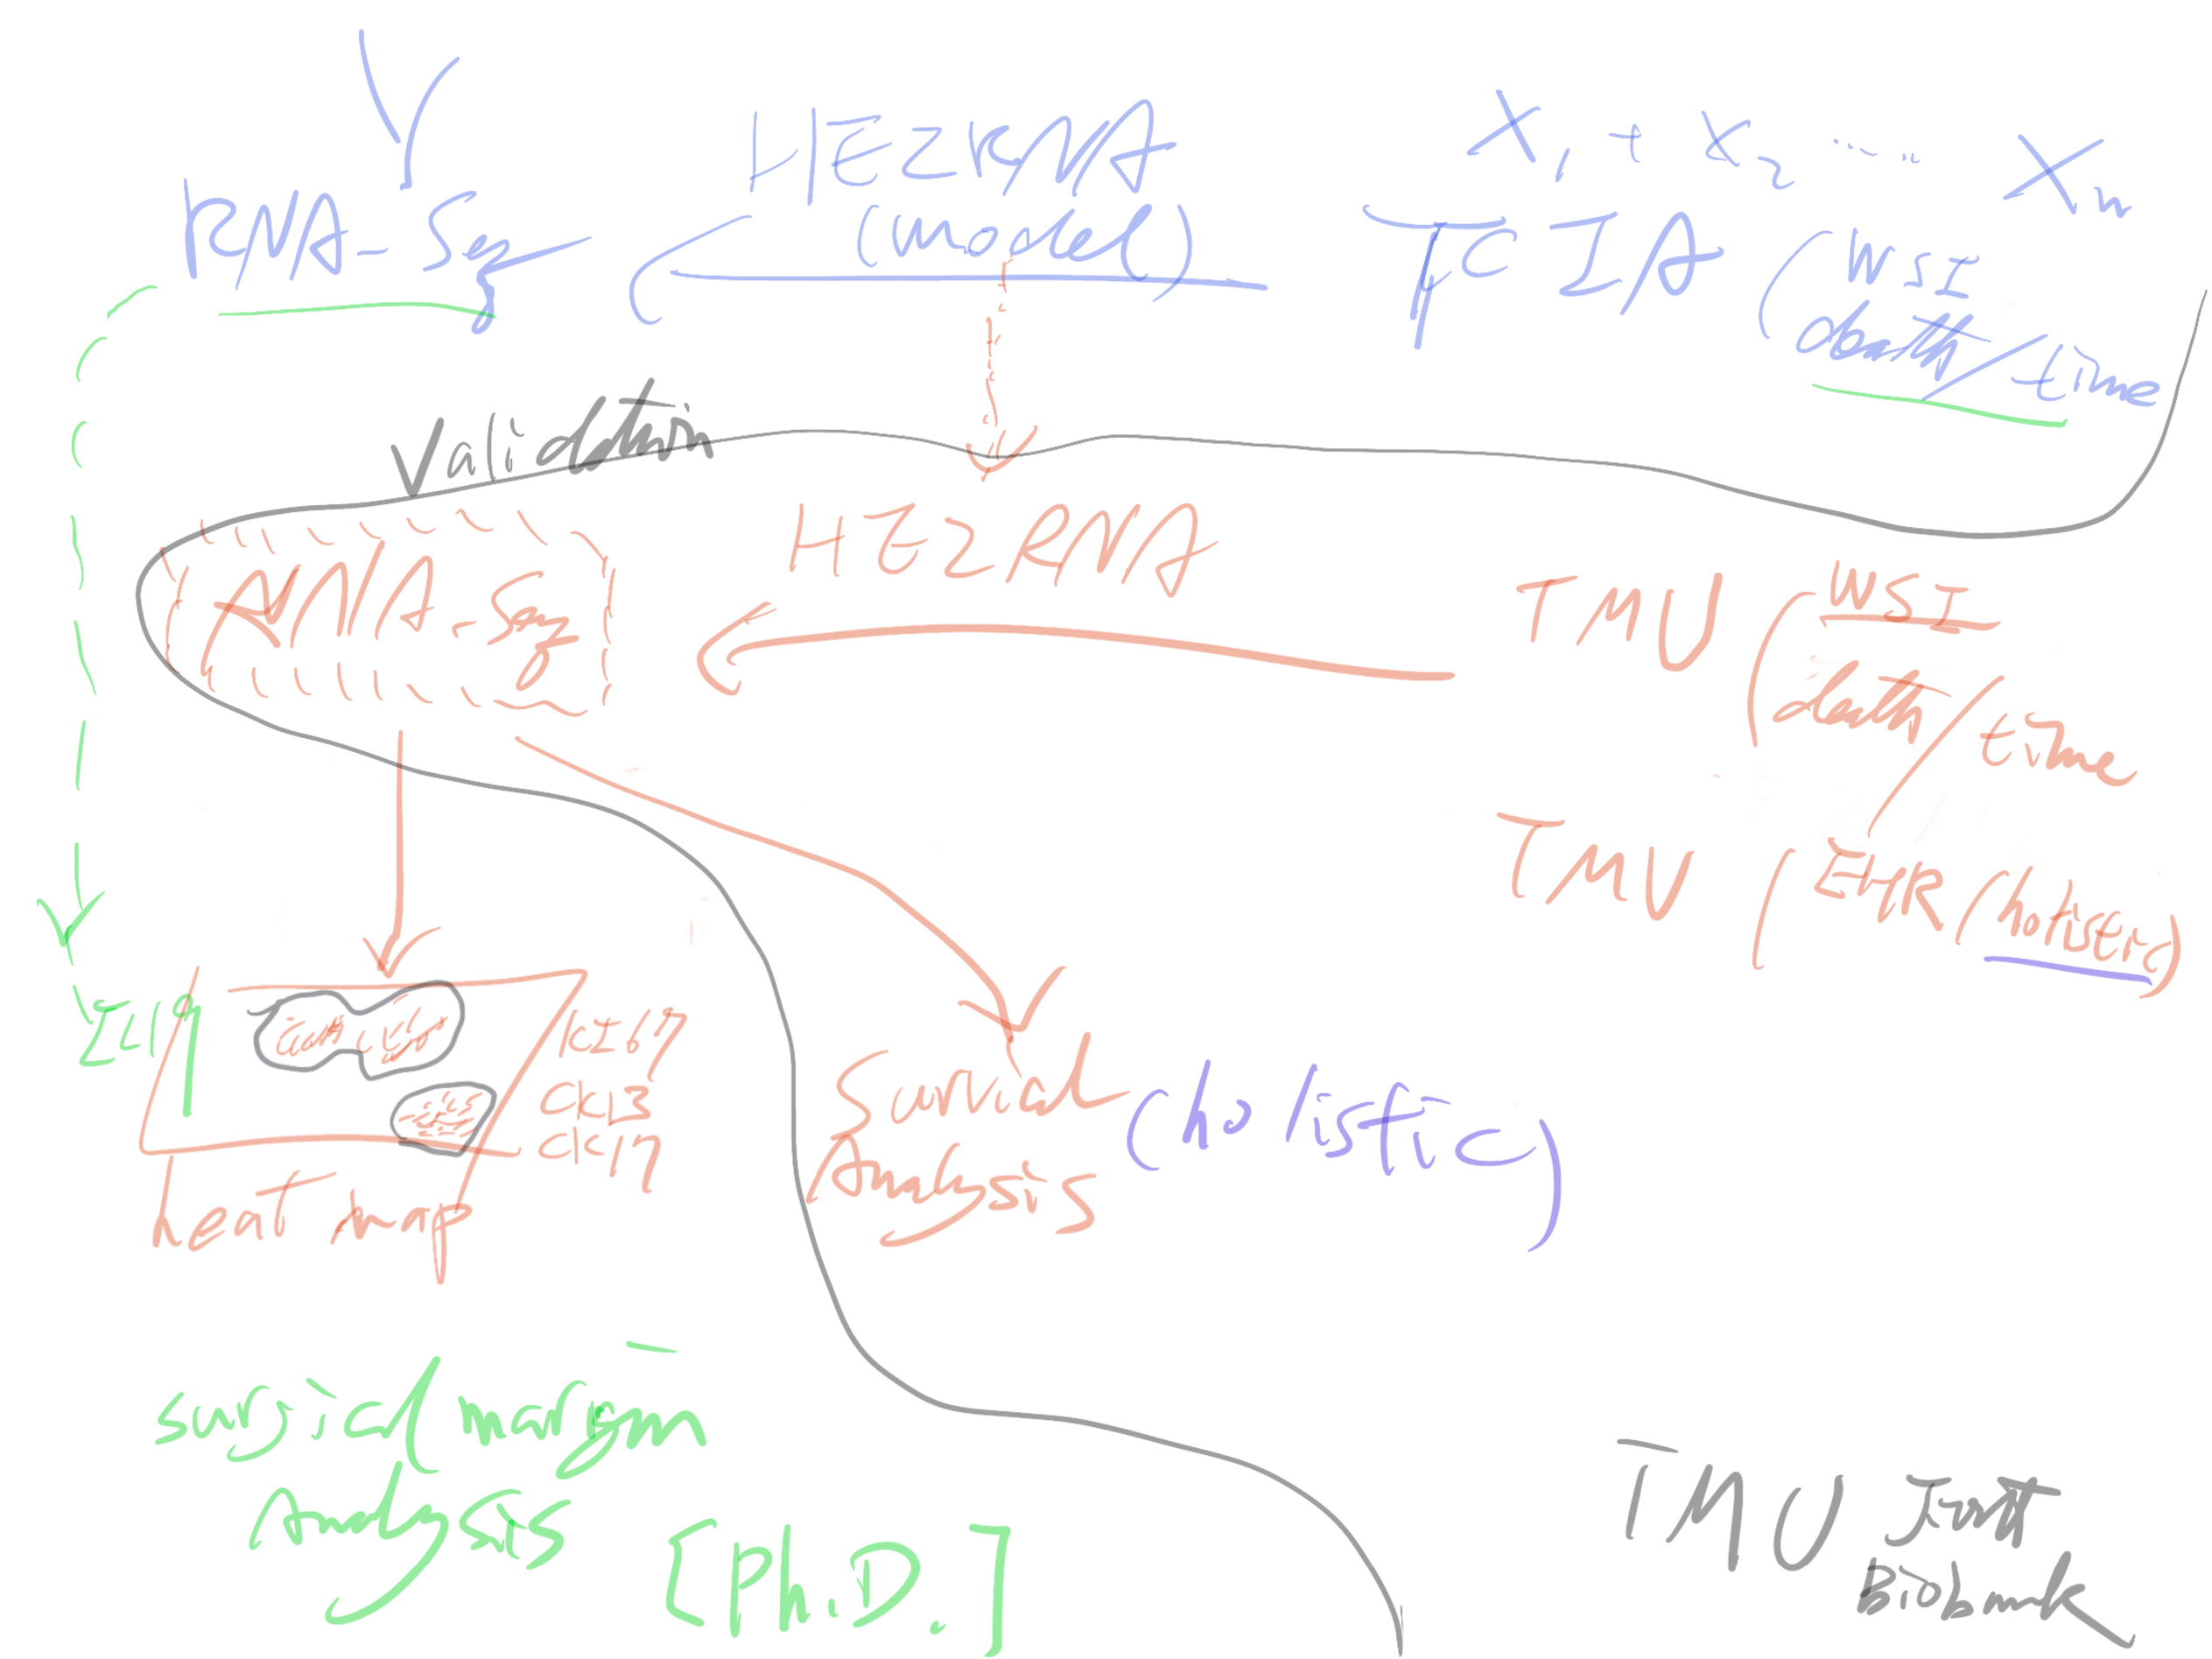
\includegraphics[width=14cm]{Figure_HE2RNA.pdf}
%\bcaption{}{} %\captionof{diag} for floating "diag"
\bcaption{Workflow of RNA-Seq representation of TMU dataset}
%\acrshort{hnscc} Cox's hazard ratio and \textit{P} value plot.
{The deep learning model of HE2RNA, which was trained under TCGA/TCIA \acrshort{hnscc} dataset, could be applied for RNA-Seq prediction of TMU dataset. The representation will be used for subsequent survival analysis.\\
(
TCGA: \acrlong{tcga};
TCIA: \acrlong{tcia};
WSI: whole-slide images of pathology
EHR: \acrlong{ehr}
RNA-Seq: \acrlong{rnaseq}
)
} %uncorrected \textit{P} value.}
\label{fig:HE2RNA}
\end{figure}
%\end{center}

\clearpage


%%%%
%\begin{outline}
\subsubsection{Aim 2:} Construct a Deep Learning Platform of Survival Analysis with EHR\\[0.5cm]
%\end{outline}
%central issue 2 with preliminary data (Cox model); fallback approaches % 需有充分的文獻分析和縝密的論述來補足,使得 “convincing power” 依然強而有力



%% TCGA new holistic features %%%%%
%Our previous \acrshort{hnscc} study\cite{Chi2020} 
Our preliminary research data summarizes that 20 candidate biomarkers, clinical T stage, and surgical margin are independent prognosis factors.
The prognosis model with coefficients is established from \acrshort{tcga} \acrshort{hnscc} cohort. The important input $X_1...X_n$ should be patients' features: age, candidate gene expressions, clinical T stage, and surgical margin so far.
When we consider the survival prediction model in a holistic manner,
ground truth Y (e.x. patient's survival):\\[0.5cm]
%Y$:\\[0.3cm]
$Y = \beta_0 + \beta_1 X_1 + \beta_2 X_2 + \beta_3 X_3 + ... + \beta_n X_n + \epsilon$\\[0.3cm]
Actually, gene expression is not an independent $X_{mrna}$. It could be influenced with other factors (for example):\\[0.3cm]
$X_{body}, X_{stress}, X_{fear}, X_{meaningOfLife}, X_{inflammation}, X_{empathy}$\\[0.3cm]
That is because there is much work to be done in investigating the functional mind-body network\citep{Rogers1959}.
%We wish the TCGA does collect more holistic features from their participants in the future.
%依舊是以管窺天
% https://link.springer.com/referenceworkentry/10.1007%2F978-1-4419-1428-6_575
%癌症與身心靈的重要關係:中醫、citation? emotional centered approach
We suggest TCGA should cover more holistic features:
The cortisol is one of the most common objective outcomes studied in psychoneuroimmunological (PNI) factor. Interleukin, cytokines, lymphocytes (CD4+, CD8+), CD56+, vitals signs, telomere length, telomere activity, and heart rate variability (HRV) are others.
The subjective psychosocial measures should include depression, stress, quality of life, anxiety, fatigue, mindfulness, mood, and specific spiritual growth (i.e., the meaning of life)\citep{Hsiao2012}.
%冤親債主的意念 unknown X factors 回到我們的文章
Since psychological benefit (reduction of stress, fatigue, sleep disturbance, and depressive symptoms) also optimizes immune function (higher natural killer cell activity, higher \acrshort{ifng}, lower TNF-alpha, lower IL-6) in terms of better survival of patients from cancer.

% holistic EHR
Moreover, we encourage physicians to write their \acrshort{ehr} in a "holistic way".
% Deep Patient:  
Thus, deep learning can convert EHR to the Fast Healthcare Interoperability Resources (FHIR) format\citep{Rajkomar2018}\citep{HealthLevelSeven2019} for handling free-text notes by physicians.
Deep learning can also derive patient representations that offer improved clinical predictions\citep{Miotto2016}.
%=> Level 4 Record-keeping and Data Exchange for the healthcare process (clinical data) %Under HL7, RESTful
%Allergy, Problem,
%Procedure,
%CarePlan/Goal,
%ServiceRequest,
%Family History,
%Risk Assessment (APGAR, Glasgow coma scale)
%condition: physical, mental
%{observations: 
%vital signs, 
%body temperature, body weight and body height, 
%x-ray, 
%laboratory data, 
%pulse oximetry, 
%ECG, EEG, EMG, 
%clinical findings (symptom and sign), 
%tobacco exposure, family support, cognitive status and pregnancy status.
%death assertion
%HIV, HBV, HCV status
%}
%https://mos2718.github.io/FHIRspec/Index.html
%https://www.hl7.org/fhir/patient.html
%https://mos2718.github.io/FHIRspec/Spec/Patient/EHR_Patient.docx
Once the holistic feature is available, a graph convolutional neural network (GCNN) is mandatory for further survival analysis\citep{Ching2018a}.

In Taipei Medical University Hospital, holistic-enabled EHR has been designed in the daily-work for charting our outpatients with psycho-social-spiritual evaluation\citep{Ling-ChengMong2021}:\\

\begin{outline}

\1 Emotional: stable/depression/ anxiety/ agitated/ perplexed\\
\1 Interaction: expression disorder/ confusion/ hard to make decision/ uncooperative to dental treatment\\
\1 Social: (disturbing living/ disturbing working/ disturbing other life aspect)\\
\1 Function loss(subjectively): mastication/ pronunciation/ life quality/ state of mind\\
\1 Self-expectation: lack of confidence/ low self-esteem/ social-withdrawal\\
\1 Impact to life: financial problem/ family problem\\
\1 Medical relationship: bad experience of dental treatment/ loss confidence to dentist/ anxious to treatment/ side-effects/ litigation experience\\[0.1cm]

\end{outline}
%In personal history section of admission note for inpatient:\\
%<Habits>\\
%-Tobacco: \underline{ }\underline{ } pack/day for \underline{ }\underline{ } years\\
%-Alcohol drinking: Occasionally\\
%-Betel nuts: \underline{ }\underline{ } nuts/day for \underline{ }\underline{ } years\\
%<Social/Economic Evaluation>\\
%-Living condition: Living with family\\
%-Family support: Well\\
%-Main caregiver: Spouse\\
%-Financial support: Sufficient\\
%<Psychological Evaluation>\\
%Stable but worry about this oral lesion\\
%Suspected to be abuse or neglected victim: negative\\
%<Spiritual Assessment>\\
%Religion: Nil\\
%Diagnosed with life-threatening diseases or terminal stage of chronic diseases or cancers? No


%子計畫 升格為主計畫 EHR of TMU Joint Biobank
%\1 Aim 3: Biomarkers validation cohort for 10 candidates from pvalueTex project


Deep learning can convert \acrfull{ehr} to the Fast Healthcare Interoperability Resources (FHIR) format\citep{Rajkomar2018}\citep{HealthLevelSeven2019} for handling free-text notes by physicians.
% RNN recurrent neural network
\acrfull{rnn} will deal with "holistic features" from \acrshort{ehr} of TMUH.
These patient's features should include physical, pathological, psychological data, and even more spiritual information investigated by physicians.



\subsubsection{Aim 3:} Biomarkers Discovery from RNA-Seq, Whole-slide Images, and EHR from TMU dataset\\[0.5cm]

%\1 Aim 3: RNA-Seq Incorporated with Whole-slide Images models from TCIA and TMU\\
%central issue 3 without preliminary data; fallback approaches

%\begin{outline}
Whole-slide images are the surrogate of expression data of RNA-Seq.
From the result of Aim 1, the transcriptomic representation of TMU dataset (n=46, obtained at TMU Joint Biobank) could be applied to validate those candidates discovered by our previous study.
% Biomarkers validation cohort for 10 candidates from pvalueTex project
Moreover, the result of Aim 2 (features extracted from holistic \acrshort{ehr} of TMUH) will be used for survival analysis (see Figure \ref{fig:HE2RNA}.
% modifying % Figure 5 HE2RNA workflow

%需有充分的文獻分析和縝密的論述來補足,使得 “convincing power” 依然強而有力
%*transfer learning from TCGA model
%torchvision, NanoMets Models
%save checkpoint, load then deepcopy()


%\subsubsection{TCIA validation by deep learning}
%https://www.cancerimagingarchive.net/
%from CPTAC and TCGA images
%poster 
%https://wiki.cancerimagingarchive.net/download/attachments/1966514/TCGA_TCIA_Poster_111511_HHFa_WIDE.pptx?version=1&modificationDate=1323207330686&api=v2



%\end{outline}









\clearpage



%%%%%%
%\include{chapter0}
%\include{chapter1} % introduction
%\include{chapter2} % Review of Literature
%\include{chapter3} % Methodology (Research Design & Methods)
%\include{chapter4} % Results (Presentation of Research) C004 or C005...
%%%%%

\section{\cntext{(三)預期完成之工作項目、成果及績效}}
%1.預期完成之工作項目
Validation of candidate biomarkers of HNSCC by TMU Biobank.
%2.對於學術研究、國家發展及其他應用方面預期之貢獻
for further drug development of systemic therapy of HNSCC (personalized medicine ) or \cntext{精準醫療}
%3.對於參與之工作人員,預期可獲之訓練
to improve the PyTorch and C ++ programming skill
%4.預期完成之研究成果及績效(如期刊論文、研討會論文、專書、技術報告、專利或技術移轉等質與量之預期績效)。請詳述其必要性以及預期成果等。
We will write Ph.D. dissertation as well manuscript for SCI publication.

\clearpage

\section{\cntext{計畫經費之編列}}
% 核定的經費不會高於所 要求的預算,如經費不足對日後計畫執行也是障礙,因此每項經費的使用最好 想清楚,說明白,比如設備費,逐年需購買哪些圖書?何以需購買電腦、筆 電,尤其國立大學設備資源較充裕,平均四年即更新汰舊電腦,編列時還經常 可見便宜行事的情況,複製經費編列,以致於每年都購買電腦或印表機,顯見 並不適合。參與國際會議及移地研究,停留天數及其必要性都需填寫,說明越 清楚,通過的機會就越高。此外,編列項目越詳細越好,免得日後有需要時, 因計畫書未列,校方不准核銷,而影響計畫的進行。
The third page looks like this. 
%主要研究人力,主持人每周平均投入工作時數比例,請「合理」。(100% 就是不合理喔!!請注意。一般而言,20-40%或 50%是比較合理)
\begin{outline}


%計畫主持人得依計畫實際需要,申請下列各項補助款。
% https://research.nchu.edu.tw/upfile/editor/files/科技部補助專題研究計畫耗材物品圖書及雜項費用及研究設備費支出用途範例.pdf

\1 \cntext{業務費}
\2 \cntext{研究人事費:}
%含研究助理費及臨時工資等,以科技部補助專題研究計畫助理人員工作酬金支給標準為核定依據: Ph.D. candidate 34,000 per month (2,000 x 17 units)

\2 \cntext{研究主持費:}
% 近五年內研究績效優異者,得編列研究主持費,經計畫審查小組審核通過後,每人至多核給每月新台幣一萬元 。計畫主持人或共同主持人於研究計畫執行期間僅得由此補助 辦法支領一份研究主持費。於研究計畫執行期間,因離職、轉 任或無法執行該計畫時,即停止核發研究主持費。
\2 \cntext{耗材費:} %消耗性器材與藥品費、問卷 調查費 及其它事務性費用(如電腦耗材費、郵電費、印刷影印費、資料檢索費、國內差旅費、論文發表費) 在核定 經費限額內核實列支
\3 \cntext{電腦使用費(使用電腦所需費用,如以執行機構出具之收據報銷,應檢附計算標 準、實際使用時數及耗材支用情形等支出 數據資料)}
\3 \cntext{資料檢索費(使用傳輸網路所供應新穎數據或索取各交換系統資料庫中之資料所需費用)}
\3 \cntext{網路使用費}
\3 \cntext{資料庫使用費}
\3 \cntext{問卷調查費(實地調查訪問及搜集各種資料所需費用)} 
\3 \cntext{受試者禮品、營養品及交通費}
\3 \cntext{國內或國際性學會之年費或入會費}
\3 \cntext{論文發表費(本部補助研究計畫之研究成果發表於國內外著名之學術期刊所需之相關費用)}
\3 \cntext{研究計畫相關實驗進行之審查費(如人體試驗委員會等審查費)}
\3 \cntext{翻譯及潤稿費}
\3 \cntext{會議餐費(因研究計畫需要召開會議而逾用餐時間所提供之餐點)}
\3 \cntext{田野調查之茶點費}
\3 \cntext{計畫相關之教育訓練費}
\3 \cntext{研究計畫所需的圖書(購置之圖書是否列入財產,由執行機構依「圖書館法」及「財物標準分類」有關財產與非財產之規定辦理)}
\3 \cntext{有關網站建置、程式設計和拍攝影片、實作等相關費用}
\3 \cntext{物品(非屬研究設備者)} 
\3 \cntext{印刷與影印費}
\3 \cntext{文具}
\3 \cntext{紙張}
\3 \cntext{郵電費}


\1 \cntext{研究設備費:} 
\cntext{資訊硬體設備 1 to 2 萬元} %在核定 經費限額內核實列支
% 凡執行研究計畫所需單價在新台幣一萬元以上且使 用年限在二年以上之各項儀器、機械及資訊設備(含各項電腦設 施、網路系統、周邊設備、套裝軟體、程式設計費)等之購置、 裝置費用及圖書館典藏等,本項設備之採購,以與研究計畫直接 有關者為限,研究設備費補助金額不得超過總補助經費20%
\1 \cntext{管理費:} % 5% 為執行機 構配合執行研究 計畫所需之費 用,由執行機構統 籌支用
\end{outline}


%\section{\cntext{對社會的貢獻}}

\section{\cntext{過去研究之表現}}
% 申請人過去五年著作及五年以上且深具影響之著作,最好詳細? 精簡
% * 系統的關聯性 for one researcher
%而有條理地說明自己近五年來研究的系統性、延續性以及對學界的貢獻,如果 能列出每篇論文被引用的次數,或哪些重要期刊論文曾引用,可以更凸顯自己 的優勢,爭取更有利的評分。個人學術表現既如此重要,因此每一次的申請都 應記得更新個人資料 C302 表,確認與完成登錄著作目錄之作業,產生近 5 年著 作目錄表
We applied the matrix-assisted laser desorption/ionization (MALDI) imaging mass spectrometry (IMS) and liquid chromatography with tandem mass spectrometry (LC-MS/MS) to identify tumor-associated biomarkers of \acrshort{hnscc}. The gene thymosin beta-4 X-linked (TMSB4X) is a candidate biomarker in HNSCC whose functions resulted in enhanced proliferation and metastasis in vitro and in vivo\citep{Chi2017}.
This publication has been cited by cancer research of Roška and his colleague, published on Oncotarget\citep{Roska2020}, \citep{Chu2019a}, \citep{Makowiecka2019a}, and by research of epidermal morphogenesis\citep{Padmanabhan2020}.
 % ------------------------------------------------------
%
% References
%
% ------------------------------------------------------
 \clearpage
\renewcommand\bibsection{\section*{REFERENCES}}
\setlength{\bibsep}{2pt}
%\bibliography{IEEEabrv, pvalueTex, TMSB4X, TCGA_margin_cutoff, SLC2A4_metabolism.bib, Holistic, Deep_Learning-Radiomics, Deep_Learning}
% all merged at most_merged, repeated entry removed
\bibliography{most_merged}
% by
% $ bibtool -f '%s($key)' -Ac -s -v /Users/texchi/Documents/Documents\ -\ Mac\ mini/Holistic.bib /Users/texchi/Documents/Documents\ -\ Mac\ mini/Deep_Learning.bib /Users/texchi/Documents/Documents\ -\ Mac\ mini/pvalueTex.bib /Users/texchi/Documents/Documents\ -\ Mac\ mini/SLC2A4_metabolism.bib /Users/texchi/Documents/Documents\ -\ Mac\ mini/TMSB4X.bib /Users/texchi/Documents/Documents\ -\ Mac\ mini/TCGA_margin_cutoff.bib -o most_merged.bib$
\end{document}


%%%%%%%%%%%%%%%%%%%%%%%%%%%%%%%%
%\smartdiagramset{uniform sequence color=true}
% sequence diagram; flow diagram:horizontal
% 2021
\smartdiagram[sequence diagram]{2021/July, Aug, Sep, Oct, Nov, Dec}

\smartdiagramset{border color=none,
   set color list={blue!50!cyan,green!60!lime,orange!50!red,red!80!black},
   back arrow disabled=true}

\smartdiagramset{module x sep=5}
\smartdiagram[flow diagram:horizontal]{Aim1, Aim1}


\smartdiagramset{border color=none,
   set color list={blue!50!cyan,green!60!lime,orange!50!red,red!80!black},
   back arrow disabled=true}
\smartdiagramset{module x sep=5}
\smartdiagram[flow diagram:horizontal]{Aim1, Aim2, Aim3}

% 2022
\smartdiagram[sequence diagram]{2022/Jan, Feb, March, April, May, June}

\smartdiagramset{module x sep=15}
\smartdiagram[flow diagram:horizontal]{Aim3, Aim4}
%\end{center}


%%%%%%%%%%

\paragraph{Immune System and Cancer}
% balanced Yan and Yin 陰陽要調合
Two-faced roles of tumor-associated neutrophils, eosinophils, and basophils

*** Tex's opinion: there is no "central console" of immune control system, which disseminated remote regular % 地方自治 

chronic inflammation by mechanical force or chemicals

** or even in autoimmune disease:
Risks from disease and treatment
Autoimmune disorders generally attack a single organ or part of the body, often causing inflammation in the affected area. In some cases, that inflammation may increase cancer risk. 
At the same time, tumor necrosis factor (TNF) inhibitors or immunosuppressant (e.x. cyclosporin), help reduce inflammation and also are suspected of increasing the risk of multiple cancers. It may impair the ability to kill cancer cells.

two of ten hallmarks: avoiding immune destruction, tumor-promoting inflammation \citep{Ohman2015}



The basic principles that guide cancer immunology are immune surveillance \citep{BURNET1957, Shankaran2001}, immune editing, and immune tolerance.
%immunosurveillance
Peritumoral immune responses might predict patients’ prognosis in a wide range of cancers. Beyond local accumulation, systemic immune response in serum is seen in patients with \acrshort{hnscc} \citep{Lee2010a}.
% immunoediting 敵消我長的過程
Moreover, the immune response is not only achieving protection of the host but also editing the immunogenicity of tumours \citep{Dunn2002}.
The cancer immunoediting includes elimination, equilibrium then escape.
%elimination by immunosurveillance
The cells, which have aberrant major histocompatibility complex (MHC) class I expression, will be eliminated by cytotoxic mechanism or induction of apoptosis by immune cells, involving granulocytes (neutrophils, eosinophils, and basophils), macrophages, natural
killer cells, in innate immunity \citep{Tallerico2013}.
Tumour-associated macrophages include  M1, which has antitumoral properties, and M2, which has tumour-promoting phenotype in \acrshort{hnscc} \citep{Kumar2019}.

Through dendritic cells presenting the tumor antigens to T helper cells in context with MHC class II molecules, naive or memory T cells will conduct activation of  T cells and adaptive immunity \citep{Banchereau2000}. 
The plasmacytoid cells are a subtype of dendritic cells that are one of the main sources of secreting \acrshort{ifng}. 
T cells consist of at least five subgroups: Th1 (CD4+), Th2 (CD4+), Th17 (CD4+), regulatory T cells (CD4+ CD25+ Tregs), and cytotoxic T cells (CD8+). 
Cytotoxic T cells is triggered by helper T cells to attack directly and execute those tumor cells, whose antigen is presented by dendritic cells, via effector molecules such as perforin and granzyme. Cytotoxic T cells also use TRAIL receptor to release signal on tumor's FasL to induce cell apoptosis.
% By inducing intracellular signaling through lck, the CD8 coreceptor is an important factor affecting TCR‐mediated T cell activation and modulation of immunosuppression and cytotoxicity.
All subsets play important roles in mucosal immune response, including antitumoral responses. T cells represent approximately 10\% of the total cells in a tumour mass \citep{Balkwill2012}.

% equilibrium under immunoselection:  Cancer cells avoid immunosurveillance by the selection of non-immunogenic tumour-cell variants % 鄭爺爺
***When immunosurveillance systems are not able to eradicate the tumor cells, the result may be tumor dormancy, where an equilibrium with defending cells occurs.

equilibrium represents a time of tumour cell persistence without progression.
equilibrium is maintained solely by adaptive immunity
The interplay of the potentially malignant cells and immune cells from immunosurveillance, equilibrium to tumor escape.
Lymphocytes of adaptive immunity have the capacity to take over and exert enough antitumoral effects to kill and limit tumour growth, and the tumour is thus kept in their dormitory \citep{Koebel2007}.
The tumour cells in equilibrium are highly immunogenic (unedited), whereas those spontaneously exiting equilibrium (escape) that become growing tumours have attenuated immunogenicity (edited)—results that place this process temporally between elimination and escape \citep{Koebel2007}.
maintaining cancer in an equilibrium state may represent a relevant goal of cancer immunotherapy in which augmentation of adaptive tumour immunity could result in improved tumour control. *** A TREATMENT GOALS
%the downregulation or loss of expression of HLA class I molecules
% decoy receptors for TRAIL: DcR3, Decoy receptor 3 (DcR3), to prevent FasR-FasL interactions by competitively binding to membrane-bound Fas ligand; FasL binds to DcR3 (TNFRSF6B) without TRAIL function 假的誘餌
% Death receptors:  tumour-necrosis-factor (TNF) receptor 1, CD95 (also known as FAS) and two receptors for TNF-related apoptosis-inducing ligand (TRAILR1 and TRAILR2).


% escape under immunesubversion: by the active suppression of the immune response
Escape is the process wherein the immunologically sculpted tumor expands in an uncontrolled manner in the immunocompetent host \citep{Dunn2002, Dunn2004}.
It was suggested by increasing the presence of Tregs in terms of suppression of Th1 and cytotoxic T cells response by \acrfull{ctla4} \citep{Halvorsen2014}.
Moreover, myelo-derived suppressor cells (MDSCs, CD34+) could also down-regulation of granzyme from T cells in \acrshort{hnscc} \citep{Si2019}.
The antitumoral effect of adaptive immunity also help to the tumour evolution. It lets tumour cells to modify immunogenicity to avoid immune recognition, and to resist the cytotoxicity of T cells.
The activated oncogenes can trigger 1) DNA-damage sensors, [such as ATM (ataxia-telangiectasia mutated) and ATR (ATM and Rad3 related)]; 2) checkpoint kinases, [such as CHK1 (checkpoint kinase 1 homologue) and CHK2]; 3) and the tumour-suppressor protein p53. 
The transcription factor, p53, that is activated by many genotoxic insults and induces cellular apoptosis. The gene TP53, encoding p53, is frequently mutated or functionally inactivated in cancer cells.
Through suppression of the DNA-damage response by above mechanisms, tumor cells might downregulation of NKG2D ligands (\acrshort{mica}, \acrshort{micb}) to avoid recognition by NKG2D-expressing NK cells, natural killer T (NKT) cells, $\gamma\delta$ T cells and some cytolytic CD8+ $\alpha\beta$ T cells \citep{Ljunggren2007}. They also express PD‐L1 and Fas ligand to suppress cytotoxic T cells \citep{Zitvogel2006}. Thus, the cell-cycle arrest, DNA repair or apoptosis (aka. DNA-damage response) of tumor cells will be inhibited.
The activation of $\acrshort{tgf}\beta$ in terms of promoting epithelial-to-mesenchymal transition (EMT). 
%IL-10
% Activation of the DNA-damage response by cell-intrinsic stimuli (oncogene activation or reactive oxygen species, ROS) or therapy activates the ATM (ataxia-telangiectasia mutated)–CHK1 (checkpoint kinase 1 homologue) pathway. This pathway leads either to p53- or NKG2D- (ligand: MICA or MICB) dependent apoptosis of tumour cells.
% NKG2D (Natural-killer group 2, member D). A lectin-type activating receptor that is encoded by the NK complex and is expressed at the surface of NK cells, NKT cells, γδ T cells and some cytolytic CD8+ αβ T cells. 
% The ligands for NKG2D are MHC-class-I-polypeptide-related sequence A (MICA) and MICB in humans; and retinoic acid early transcript 1 (RAE1) and H60 in mice

% 小巷弄防巷戰 (金門防線)
Finally, tumor cells have downregulated homing receptors, and malformation of peripheral vacularity. It causes hypoxia and increased interstitial pressure which lead to a hostile microenvironment for against the infiltrating defense cells \citep{Ljunggren2007}.


%{ references
ICI, hallmarks of cancer
%** Sharma, P. et al. Cancer Immunotherapy. in Holland‐Frei Cancer Medicine 1–23 (John Wiley & Sons, Inc., 2017). doi:doi:10.1002/9781119000822.hfcm068.

%**1. Öhman, J. Potentially Malignant Disorders and Oral cancer -A study on Immunosurveillance. GUPEA (University of Gothenburg. Sahlgrenska Academy, 2015). doi:10.16880/sec.2015.58.01.107.
https://gupea.ub.gu.se/handle/2077/37523 a dissertation of HNSCC
%gupea_2077_37523_4.pdf

There is 5 papers for this dissertation. :-)
The concept of immunosurveillance originally proposed by Dunn et al. in 2004 is well in line with the findings in this thesis of PMOD and oral cancer.

%** Cillo, A. R., Kürten, C. H. L., Tabib, T., Qi, Z., Onkar, S., Wang, T., … Vignali, D. A. A. (2020). Immune Landscape of Viral- and Carcinogen-Driven Head and Neck Cancer. Immunity, 52(1), 183-199.e9. https://doi.org/10.1016/j.immuni.2019.11.014
HPV or chemicals (with Graphical Abstract)

%%
%% 
Evasion of apoptosis contributes to the acquisition of initial oncogenesis, resistance to chemotherapy and to immune effectors
The apoptotic program is carried out through two main pathways: the mitochondrial pathway, which involves mitochondrial outer-membrane permeabilization (MOMP)61; and the death-receptor pathway, which involves ligation of a plasma-membrane receptor, leading to the formation of a death-inducing signalling complex (DISC).

% a long way to go becoming cancer
Chronic inflammation is a risk factor in promoting carcinogenesis. The persistent inflammation in oral lichen planus (with reticular striations) was found that the influx of T helper, cytotoxic T cells, and B cells were increased in oral mucosa with moderate to severe dysplasia and oral squamous cell carcinoma compared to normal or mild dysplasia \citep{Gannot2002}. The infiltration of T cells and dendritic cells were also found in oral lichen planus \citep{Lorenzini2013}.
The incidence of malignant transformation of oral lichen planus is approximately 0.5–1.5\% \citep{Bermejo-Fenoll2009}, while oral leukoplakia is about 10\%.

%%%
\begin{table}
%\begin{sidewaystable}[hp]
\centering
\caption{ The top 10 genes overexpressed with poor prognosis in \acrshort{hnscc} (ranked by Bonferroni adjusted \textit{P} value) }
\arrayrulecolor[rgb]{0.255,0.255,0.255}
\resizebox{\linewidth}{!}{
%\begin{tabular}{|l|l|l|l|l|l|l|l|c|}
\begin{tabularx}{\textwidth}{|l|p{3.5cm}|l|l|l|l|l|l|c|} % *** capital X or p{2cm}
% p{2cm}
\hline
\multicolumn{1}{|c|}{\multirow{2}{*}{Gene ID}} & \multicolumn{1}{c|}{\multirow{2}{*}{Gene Description}}     & \multicolumn{2}{c|}{Kaplan-Meier survival}                                                                                   & \multicolumn{2}{c|}{Univariate~}                                                        & \multicolumn{2}{c|}{Multivariate}                                                       & \multirow{2}{*}{Remark}                     \\ 
\cline{3-8}
\multicolumn{1}{|c|}{}                         & \multicolumn{1}{c|}{}                                      & \multicolumn{1}{c|}{\textit{P} value}               & \multicolumn{1}{c|}{\begin{tabular}[c]{@{}c@{}}Adjusted \\\textit{P} value\end{tabular}} & \multicolumn{1}{c|}{HR*}                   & 95\% CI                                    & HR*                                        & 95\% CI                                    &                                             \\ 
\hline
DKK1                                           & dickkopf WNT signaling pathway inhibitor 1                 & \num{8.9e-8}                               & 0.001                                                                           & 2.266                                      & 1.666-3.082                                & 2.135                                      & 1.559-2.924                                &                                           \\ 
\hline
CAMK2N1                                        & calcium/calmodulin-dependent protein kinase II inhibitor 1 & \num{2.9e-7}                               & 0.002                                                                           & 2.101                                      & 1.572-2.809                                & 2.007                                      & 1.490-2.704                                & \checkmark                                          \\ 
\hline
STC2                                           & stanniocalcin 2                                            & \num{6.5e-7}                               & 0.004                                                                           & 2.147                                      & 1.578-2.921                                & 2.075                                      & 1.515-2.843                                &                                           \\ 
\hline
PGK1                                           & phosphoglycerate kinase 1                                  & \num{9.1e-7}                               & 0.006                                                                           & 2.127                                      & 1.563-2.895                                & 2.046                                      & 1.498-2.795                                & \checkmark                                          \\ 
\hline
SURF4                                          & surfeit 4                                                  & \num{9.6e-7}                               & 0.006                                                                           & 2.055                                      & 1.531-2.757                                & 2.089                                      & 1.543-2.829                                & \checkmark                                           \\ 
\hline
USP10                                          & ubiquitin specific peptidase 10                            & \num{1.7e-6}                               & 0.012                                                                           & 2.083                                      & 1.532-2.834                                & 2.119                                      & 1.551-2.895                                & \checkmark                                         \\ 
\hline
NDFIP1                                         & Nedd4 family interacting protein 1                         & \num{2.6e-6}                               & 0.017                                                                           & 2.031                                      & 1.502-2.746                                & 2.027                                      & 1.483-2.771                                & \checkmark                                           \\ 
\hline
FOXA2                                          & forkhead box A2                                            & \num{2.7e-6}                               & 0.018                                                                           & 1.976                                      & 1.479-2.640                                & 1.914                                      & 1.426-2.569                                & \checkmark                                          \\ 
\hline
STIP1                                          & stress-induced-phosphoprotein 1                            & \num{4.3e-6}                              & 0.029                                                                           & 1.958                                      & 1.463-2.621                                & 1.957                                      & 1.451-2.640                                &                                           \\ 
\hline
DKC1                                           & dyskeratosis congenita 1, dyskerin                         & \num{6.3e-6}                               & 0.042                                                                           & 2.046                                      & 1.490-2.808                                & 1.837                                      & 1.332-2.534                                &                                           \\ 
\hline
\multicolumn{1}{|l!{\color{black}\vrule}}{}    & \multicolumn{1}{l!{\color{black}\vrule}}{}                 & \multicolumn{1}{l!{\color{black}\vrule}}{} & \multicolumn{1}{l!{\color{black}\vrule}}{}                                      & \multicolumn{1}{l!{\color{black}\vrule}}{} & \multicolumn{1}{l!{\color{black}\vrule}}{} & \multicolumn{1}{l!{\color{black}\vrule}}{} & \multicolumn{1}{l!{\color{black}\vrule}}{} & \multicolumn{1}{l!{\color{black}\vrule}}{}  \\ 
\arrayrulecolor{black}\hline
\multicolumn{9}{|l!{\color{black}\vrule}}{\begin{tabular}[c]{@{}l@{}}Selection criteria:~~\\~Kaplan-Meier Bonferroni adjusted \textit{P} $< 0.05 $~\\~Cox's univariate and multivariate$ HR >= 1.5$ \end{tabular}}                                                                                                                                                                                                                                                              \\ 
\hline
\multicolumn{9}{|l!{\color{black}\vrule}}{* Cox's model: \textit{P} $< 0.001$ }                                                                                                                                                                                                                                                                                                                                                                                                  \\ 
\hline
\multicolumn{9}{|l!{\color{black}\vrule}}{Remark: \checkmark validated by GSE2837}                                                                                                                                                                                                                                                                                                                                                             \\
\hline
\end{tabularx}
}
\arrayrulecolor{black}
\label{table:table1}

%\end{sidewaystable}
\end{table}


%%%

%\subsubsection{Table3/legend} or Table 2
%Table3. The 10 candidate genes overexpressed with better prognosis in HNSCC (ranked by Bonferroni corrected Kaplan-Meier P-value).
\begin{table}[hp]
\centering
\caption{The other top 10 genes overexpressed with better prognosis in \acrshort{hnscc} (ranked by Bonferroni corrected \textit{P} value) }
\arrayrulecolor[rgb]{0.255,0.255,0.255}
\resizebox{\linewidth}{!}{%
\begin{tabular}{|l|l|l|l|l|l|l|l|c|} 
\hline
\multicolumn{1}{|c|}{\multirow{2}{*}{Gene ID}} & \multicolumn{1}{c|}{\multirow{2}{*}{Gene Description}} & \multicolumn{2}{l|}{Kaplan-Meier survival}                                                                                                                                                & \multicolumn{2}{c|}{Univariate~}                                                                        & \multicolumn{2}{c|}{Multivariate}                                                                       & \multicolumn{1}{l|}{\multirow{2}{*}{Remark}}  \\ 
\cline{3-8}
\multicolumn{1}{|c|}{}                         & \multicolumn{1}{c|}{}                                  & \multicolumn{1}{c!{\color{black}\vrule}}{\textit{P} value}                                  & \multicolumn{1}{c!{\color{black}\vrule}}{\begin{tabular}[c]{@{}c@{}}Adjusted\\~\textit{P} value\end{tabular}} & \multicolumn{1}{c!{\color{black}\vrule}}{HR*}   & \multicolumn{1}{c!{\color{black}\vrule}}{95\% CI}     & \multicolumn{1}{c!{\color{black}\vrule}}{HR*}   & \multicolumn{1}{c!{\color{black}\vrule}}{95\% CI}     & \multicolumn{1}{l|}{}                         \\ 
\cline{1-2}\arrayrulecolor{black}\cline{3-8}\arrayrulecolor[rgb]{0.255,0.255,0.255}\cline{9-9}
ZNF557                                         & zinc finger protein 557                                & \multicolumn{1}{l!{\color{black}\vrule}}{\textcolor[rgb]{0,0,0.471}{\num{8.6e-8}}} & \multicolumn{1}{l!{\color{black}\vrule}}{0.001}                                                      & \multicolumn{1}{l!{\color{black}\vrule}}{0.465} & \multicolumn{1}{l!{\color{black}\vrule}}{0.348-0.619} & \multicolumn{1}{l!{\color{black}\vrule}}{0.499} & \multicolumn{1}{l!{\color{black}\vrule}}{0.372-0.669} &                                              \\ 
\cline{1-2}\arrayrulecolor{black}\cline{3-8}\arrayrulecolor[rgb]{0.255,0.255,0.255}\cline{9-9}
ZNF266                                         & zinc finger protein 266                                & \textcolor[rgb]{0,0,0.471}{\num{2.2e-7}}                                           & 0.001                                                                                                & 0.474                                           & 0.355-0.632                                           & 0.453                                           & 0.338-0.607                                           &                                              \\ 
\hline
IL19                                           & interleukin 19                                         & \textcolor[rgb]{0,0,0.471}{}\num{3.7e-7}\textcolor[rgb]{0,0,0.471}{}               & 0.002                                                                                                & 0.472                                           & 0.351-0.635                                           & 0.459                                           & 0.340-0.619                                           & \checkmark                                            \\ 
\hline
MYO1H                                          & myosin 1H                                              & \textcolor[rgb]{0,0,0.471}{}\num{3.8e-7}\textcolor[rgb]{0,0,0.471}{}               & 0.003                                                                                                & 0.468                                           & 0.347-0.632                                           & 0.467                                           & 0.344-0.634                                           &                                              \\ 
\hline
FCGBP                                          & Fc fragment of IgG binding protein                     & \textcolor[rgb]{0,0,0.471}{}\num{1.2e-6}\textcolor[rgb]{0,0,0.471}{}               & 0.008                                                                                                & 0.484                                           & 0.359-0.653                                           & 0.496                                           & 0.366-0.674                                           &  \checkmark                                           \\ 
\hline
LOC148709                                      & LncRNA LOC148709                                       & \textcolor[rgb]{0,0,0.471}{\num{1.5e-6}}                                           & 0.010                                                                                                & 0.499                                           & 0.374-0.666                                           & 0.485                                           & 0.361-0.652                                           &                                              \\ 
\hline
EVPLL                                          & envoplakin-like protein                                & \textcolor[rgb]{0,0,0.471}{\num{2.0e-6}}                                           & 0.013                                                                                                & 0.490                                           & 0.363-0.661                                           & 0.494                                           & 0.364-0.672                                           &                                              \\ 
\hline
PNMA5                                          & paraneoplastic antigen like 5                          & \textcolor[rgb]{0,0,0.471}{\num{2.6e-6}}                                           & 0.017                                                                                                & 0.499                                           & 0.371-0.671                                           & 0.481                                           & 0.357-0.650                                           &                                              \\ 
\hline
KIAA1683                                       & new name as IQ Motif Containing N (IQCN)                           & \textcolor[rgb]{0,0,0.471}{\num{3.1e-6}}                                           & 0.020                                                                                                & 0.500                                           & 0.371-0.673                                           & 0.483                                           & 0.356-0.654                                           &   \checkmark                                           \\ 
\hline
NPB                                            & neuropeptide B                                         & \textcolor[rgb]{0,0,0.471}{\num{4.0e-6}}                                           & 0.027                                                                                                & 0.460                                           & 0.328-0.646                                           & 0.457                                           & 0.324-0.646                                           &      \checkmark                                        \\ 
\hline
                                               &                                                        &                                                                                    &                                                                                                      &                                                 &                                                       &                                                 &                                                       & \multicolumn{1}{l|}{}                         \\ 
\hline
\multicolumn{9}{|l|}{\begin{tabular}[c]{@{}l@{}}Selection criteria:~\\~Kaplan-Meier Bonferroni adjusted \textit{P} value \textless{} 0.05~\\~Cox's univariate and multivariate HR \textgreater{}= 1.5\\ * Cox's model: \textit{P} value \textless{} 0.001\\lncRNA: Long non-coding RNA\\Remark: \checkmark Validated by GSE2837 ~\end{tabular}}                                                                                                                                                                                                                 \\
\hline
\end{tabular}
}
\arrayrulecolor{black}
\label{table:table3}
\end{table}


